%% Template for EU deliverable, using the deliverable.sty style file

\documentclass[12pt,a4paper,twoside]{report}

%% common package
\usepackage[headers]{deliverable}
\usepackage{xspace}
\usepackage{verbatim}
\usepackage[usenames]{color}
\usepackage[usenames,dvipsnames]{xcolor}
%\usepackage{graphicx}
\usepackage{url}
\usepackage{array}
\usepackage{graphics} 		% for pdf, bitmapped graphics files
\usepackage{graphicx}
\usepackage{epsfig} 		% for postscript graphics files
\usepackage{epstopdf}
\usepackage{caption}
\usepackage[labelformat=simple]{subcaption}
\renewcommand\thesubfigure{(\alph{subfigure})}
\usepackage{nameref}
\usepackage{multirow}
\usepackage{color}
%\usepackage{subfigure}
%%

%%insert here other packages needed by sections
%\usepackage{esint}
\usepackage{amstext}
\usepackage{amsmath}	 	% assumes amsmath package installed
\usepackage{amssymb}  		% assumes amsmath package installed
%\renewcommand\thesubfigure{(\alph{subfigure})}
\usepackage{wrapfig}
\usepackage[]{nomencl}		% nomenclatures
%\usepackage{dsfont}
%%

%%%%%%%%%%%%%%%%%%%%%%%%%%%%%%%%%%%%%%%%%%%%%%%%%%%%%%%%%%%%%%%%%%%%%%%%%%%%%%
%%% Special Commands and Packages needed by Elmar
%%%%%%%%%%%%%%%%%%%%%%%%%%%%%%%%%%%%%%%%%%%%%%%%%%%%%%%%%%%%%%%%%%%%%%%%%%%%%%
\usepackage{bm}
\usepackage{amsfonts}
\usepackage{setspace}
\usepackage{mathtools}
\newcommand{\FigureAbbr}{Fig~}%PLOS CB style
\newcommand{\FigureAbbrP}{Fig~}%PLOS CB style
\newcommand{\N}{\ensuremath{\mathcal{N}}}
\renewcommand{\vec}[1]{\ensuremath{\boldsymbol{#1}}}

%%%%%%%%%%%%%%%%%%%%%%%%%%%%%%%%%%%%%%%%%%%%%%%%%%%%%%%%%%%%%%%%%%%%%%%%%%%%%%
%%% Titlepage
%%%%%%%%%%%%%%%%%%%%%%%%%%%%%%%%%%%%%%%%%%%%%%%%%%%%%%%%%%%%%%%%%%%%%%%%%%%%%%

% declaration of variables used in style
\deliverableDocnumber{D2.2}
\deliverableTitle{Models of human whole body motions in contact with rigid and
  compliant support surfaces}

\deliverableAuthor{Morteza Azad$^{1}$, Michael Mistry$^{1}$ and Jan
  Babi\v{c}$^{2}$}
\deliverableResponsiblePartner{JSI}
\deliverableAffiliation{$^1$ School of Computer Science, University of
  Birmingham, UK.
  $^2$ Department for Automation, Biocybernetics and Robotics, Jo\v{z}ef
  Stefan Institute, Ljubljana, Slovenia.}

\deliverableReviewer{}
\deliverableCoordinator{Jan Babi\v{c}}
\deliverableActivityNumber{n} %% n=1,..,10
\deliverableActivity{Activity Name}
\deliverableDoctype{Deliverable} %% or Prototype
\deliverableClassification{Public} % or Consortium
\deliverableDistribution{Consortium} %
\deliverableStatus{Final} % Draft or Final
\deliverableDeliveryDate{29/2/2016}
\deliverableFile{Dxx\_DeliverableName.pdf} % please do not use "-" in the name
\deliverableVersion{1.0}
\deliverableDate{29/2/2016}
\deliverableYear{2016}
\deliverablePages{\pageref{LastPage}}
\deliverableChangelog{v.0.1 & Feb 04, 2016 & Initial draft %%\\\hline
%%              v.2.0 & Feb 20, 2007 & Final version
}
\deliverableProjectStartingDate{1st March 2013}
\deliverableProjectEndDate{28th February 2017}
\deliverableProjectAcronym{CoDyCo}
\deliverableProjectTitle{Whole-Body Compliant Dynamical Contacts in Cognitive Humanoids}
\deliverableContractNumber{600716}
\deliverableProjectCoordinator{Istituto Italiano di Tecnologia}
\deliverableProjectUrl{www.codyco.eu}
\deliverableFrameworkProgramme{FP7}

\deliverableWorkpackage{WP2}
\deliverableEditors{Morteza Azad, Michael Mistry and Jan Babi\v{c}}
\deliverableContributors{Morteza Azad (UB), Michael Mistry (UB), Chie
  Takahashi (UB), Elmar Rueckert (TUD), Jan Peters (TUD), Jernej \v{C}amernik
  (JSI), Jan Babi\v{c} (JSI)}
\deliverableReviewers{}
\deliverableAbstract{The scope of the current deliverable is to present the
  results on developing models of human whole body motions in contact with
  environment.}
\deliverableKeywordList{contacts, model learning, probabilistic movement
  representations}


\def\BibPath{./manuscript}       % location of bibtex-files
%%%%%%%%%%%%%%%%%%%%%%%%%%%%%%%%%%%%%%%%%%%%%%%%%%%%%%%%%%%%%%%%%%%%%%%%%%%%%%
%%% Sections
%%%%%%%%%%%%%%%%%%%%%%%%%%%%%%%%%%%%%%%%%%%%%%%%%%%%%%%%%%%%%%%%%%%%%%%%%%%%%%

%% constants
\newcommand{\botegoCaps}{BOTEGO}
\newcommand{\certhCaps}{CERTH}
\newcommand{\cybionCaps}{CYBION}
\newcommand{\nuigCaps}{NUIG}
\newcommand{\ubitechCaps}{UBITECH}

%%
%%%%%%%%%%%%%%%%%%%%%%%%%%%%%% BEGIN DOCUMENT
\begin{document}

\deliverableMaketitle

%%TODO move to style
\newcolumntype{L}[1]{>{\raggedright\let\newline\\\arraybackslash\hspace{0pt}}m{#1}}
\newcolumntype{C}[1]{>{\centering\let\newline\\\arraybackslash\hspace{0pt}}m{#1}}
\newcolumntype{R}[1]{>{\raggedleft\let\newline\\\arraybackslash\hspace{0pt}}m{#1}}

\textbf{Document Revision History}
\begin{center}
\begin{tabular}{|C{2cm}|C{3cm}|p{5cm}|C{4cm}|}
\hline
\textbf{Version}&\textbf{Date}&\textbf{Description}&\textbf{Author}\\\hline
v. 1.0 & 29 Feb 2016 & Final Version & Morteza Azad\\\hline
\end{tabular}
\end{center}
 
 \clearpage

\newpage
\renewcommand*\contentsname{Table of Contents}
\renewcommand*\listfigurename{Index of Figures}
\tableofcontents
\newpage
%\listoffigures
%\newpage

%%%%%%%%%%%%%%%%%%%%%%%% Start deliverable content here.

\chapter{Introduction}

%Short summary of our collaborative contribution

This deliverable summarizes the contribution of the CoDyCo consortium in tasks
T2.2 and T2.3 at the end of the third year.  These tasks are \textit{design of
  models for human whole body motion in contact}, and \textit{strategies of
  dealing with uncertainties in contact}, respectively.  The results are
briefly explained in four chapters.  In chapter 2, dynamic manipulability of
the centre of mass (CoM) is introduced as a metric for measuring the balance
ability of legged robots while they are in contact with their environment.
Experiments on human subjects show the applicability of this theory in
analysing balancing recovery motion in humans.  Chapter 3 investigates the use
of supporting contact (and its relationship with task) while it is required
for accomplishing a task.  In the experiments, human subjects are asked to
reach a target by the motion of one arm while they has to maintain their
postural balance with the other arm.  In a novel movement model, strong
correlations between both arms are found which were used to predict the
reaching motion solely from observing the motion related to keeping postural
stability. This finding has the potential to impact pre-tests of central
nervous system disorders that are less prone to factors like stress, sleep
deprivation and age compared to the classical cognitive tests.  In robotics,
the model can be exploited to overcome current limitations of autonomous
robots in interacting with the environment through supportive contacts.  In
chapter 4, the effects of using handles is studied for posture control of
standing subjects while they are perturbed by external forces.  It is shown
that the use of handles significantly reduces the displacement of the centre
of pressure.  Also, it is observed that subjects clearly relied on using the
handle for support, even though the perturbations did not pose a significant
balance threat.  Chapter 5 is a report of pilot study on learning compliant
contacts by human subjects.  Subjects are asked to push a complaint surface to
a certain target in order to learn the parameters of the contact.  The
compliant surface is realized by using a haptic device.  Then, in a trial
experiment, the performance of the subjects is analysed in reaching a new
target position in terms of the time needed to reach that target.


% \chapter{Executive Summary}

\chapter{Manipulability of the Center of Mass: A Tool to Study, Analyse and Measure the Ability to Balance}\label{sec:Morteza}
%%%%%%%%%%%%%%%%%%%%%%%%%%%%%%%%%%%%%%%%%%%%%%%%%%%%%%%%%%%%%%%%%%%%%%%%%%%%%%%%
%2345678901234567890123456789012345678901234567890123456789012345678901234567890
%        1         2         3         4         5         6         7         8


\newcommand{\Bq}{\mathbf{q}}
\newcommand{\Br}{\mathbf{r}}
\newcommand{\BM}{\mathbf{M}}
\newcommand{\Bg}{\mathbf{g}}
\newcommand{\Bh}{\mathbf{h}}
\newcommand{\BJ}{\mathbf{J}}
\newcommand{\BS}{\mathbf{S}}
\newcommand{\BW}{\mathbf{W}}
\newcommand{\BP}{\mathbf{P}}
\newcommand{\BI}{\mathbf{I}}
\newcommand{\BB}{\mathbf{B}}
\newcommand{\BQ}{\mathbf{Q}}
\newcommand{\BR}{\mathbf{R}}
\newcommand{\Bzero}{\mathbf{0}}
\newcommand{\Bf}{\mathbf{f}}
\newcommand{\Btau}{\boldsymbol{\tau}}
\newcommand{\EQ}{\!\!\!=\!\!\!}
\newcommand{\EQQ}{\!\!\!\!\!\!=\!\!\!\!\!\!}
\newcommand{\Bc}{\mathbf{c}}
\newcommand{\R}{\mathbb{R}}
\newcommand{\Bv}{\mathbf{v}}
\newcommand{\BD}{\mathbf{D}}
\newcommand{\BN}{\mathbf{N}}
\newcommand{\BE}{\mathbf{E}}
\newcommand{\BC}{\mathbf{C}}
\newcommand{\BA}{\mathbf{A}}


%%%%%%%%%%%%%%%%%%%%%%%%%%%%%%%%%%%%%%%%%%%%%%%%%%%%%%%%%%%%%%%%%%%%%%%%%%%%%%%%
%% \section*{Abstract}

This chapter introduces a set of metrics to study, analyse and measure the
ability to balance for both humans and legged robots.  This set of metrics,
which we call manipulability of the center of mass, are defined based on the
concept of end-effector manipulability in the literature.  Regarding the
center of mass as an end-effector and using impulsive dynamics, the metrics
are calculated to study the ability to move and accelerate this point.  They
graphically show the instantaneous change of the center of mass velocity due
to the unit weighted norm of instantaneous changes of the joint velocities or
impulses at the joints.  The proposed metrics can be computed for humans and
general legged robots with floating base and multiple contacts with the
environment in 3D space.  This chapter also provides the results of
experiments on humans to verify the application of the metrics.  In the
experiments, the centers of mass of human subjects in different configurations
are perturbed and joint torques are computed by using inverse dynamics.  The
metrics are shown to be suitable for comparing different postures in the sense
of the total required effort for balance maintenance.

%%%%%%%%%%%%%%%%%%%%%%%%%%%%%%%%%%%%%%%%%%%%%%%%%%%%%%%%%%%%%%%%%%%%%%%%%%%%%%%%
\section{Introduction}

Humans and legged robots operate in and interact with unstructured and
unpredictable environment.  The key to their safe operation is their ability
to maintain postural stability in various body configurations.  To this end,
there has been a considerable research effort in biomechanics and neuroscience
to study and understand human postural control.  Some studies investigated the
postural control in bipedal stance or walking \cite{Horak&Nashner86,
  Mergner10, Winter95}.  Other studies focused on effects of using additional
supportive contacts to the stability \cite{Babicetal14, Maki&Mcllroy97}.

In robotics many balance criteria have been proposed over the last years in
order to help to design balancing controllers.  Among them, zero moment point
(ZMP) \cite{Vukobratovic&Borovac04, Vukobratovicetal70} or center of pressure
(CoP), foot rotation indicator (FRI) \cite{Goswami99} and zero rate of change
of angular momentum (ZRAM) \cite{Goswami&Kallem04} are the most famous and
applicable ones.  Unfortunately, most of the above mentioned criteria are not
well-defined when the robot has multiple non-planar contacts with its
environment \cite{Goswami&Kallem04}.  The other problem with these criteria is
that none of them is able to distinguish between different balanced
configurations of a robot in terms of the ability to keep the balance.  In
other words, all balanced configurations for a robot are assumed to be the
same as long as they meet the balance criteria.  Here, we tackle this problem
and introduce a set of metrics that quantitatively evaluate the ability to
balance in different postural and contact configurations.  These metrics,
which are defined for both humans and robots, can also be applicable in
comparing different configurations in the sense of balance ability.

As the center of mass (CoM) plays a key role in a balancing motion, the
ability to balance, in both humans and robots, depends on the ability to move
and accelerate the CoM.  To define a set of proper metrics, we regard the CoM
as an end-effector and employ the basic concept of end-effector manipulability
in the literature \cite{Dotyetal95} and calculate a set of metrics which are
called manipulability of the CoM.  They measure the ability to accelerate the
CoM with the constant weighted norm of joint change of velocities or impulses
at the joints.

Unlike the end-effector manipulability which is a quite developed topic
\cite{Bowling&Khatib05, Dotyetal95, Guilamoetal06, Prattichizzoetal12,
  Yoshikawa85}, there have not been many studies on CoM manipulability in the
literature.  Naksuk and Lee \cite{Naksuk&Lee06} introduced ZMP manipulability
as an extension to the ZMP balance criterion based on the concept of dynamic
manipulability of end-effectors.  Then, Cotton \emph{et al.}
\cite{Cottonetal10} were the first to introduce dynamic manipulability of the
CoM for humanoid robots.  They used the motion equation of the robot to
calculate the acceleration of the CoM due to available torque at the joints.
Recently, Gu \emph{et al.} \cite{Guetal15} proposed feasible CoM dynamic
manipulability (FCDM) for planar humanoids.  To evaluate the feasibility of
the manipulability index, they considered the ground-contact force constraints
such as friction cone and unilaterlaity of the normal force.  However, their
proposed method is not developed for floating base robots with multiple
contacts.

In this chapter, we employ a different method for calculating the
manipulability of the CoM.  In this method, we do not work out the
relationship between joint torques and acceleration of the CoM by using motion
equations.  Instead, we apply impulses at the actuated joints and then compute
the relationship between the impulses (or instantaneous changes at the joint
velocities due to the impulses) and the instantaneous change of the CoM
velocity.  This is in fact the method that is used by Featherstone
\cite{Featherstone13,Featherstone15} to study the balance ability of robots on
a single point.  This approach allows us to derive a set of configuration
based metrics (i.e. velocity independent) which are applicable to all types of
legged (floating base) robots and also humans with different contact
conditions.  Therefore, these metrics provide a tool to study balancing
motions in humans and robots and also design better and more efficient robots
in the future.

In the calculation of the CoM manipulability, we take into account the effects
of inertial parameters as well as under-actuation and kinematics constraints.
The under-actuation is due to the floating base and kinematic constraints are
due to multiple contacts with the environment, such as hands and feet for
biped robots or humans.  As a result of the manipulability analysis, we obtain
two types of ellipsoids which graphically show 1) instantaneous change of the
CoM velocity due to the weighted unit norm of impulses at the actuated joints,
and 2) instantaneous change of the CoM velocity due to the weighted unit norm
of instantaneous changes of joint velocities.  These ellipsoids, which are
calculated by using impulsive dynamics, take into account the ability to cause
the motion at the CoM.  The first type of ellipsoid shows how a certain amount
of torque at the joints can accelerate the CoM.  This can be used to study the
efficiency in the sense of required torque.  The second ellipsoid shows the
ability to move the CoM with a certain amount of movement at the joints.  This
ability can be considered as maneuverability for a human or a robot: the
higher the maneuverability (larger ellipsoid), the less movement is required
to correct the position of the CoM.

In order to investigate the applicability of the proposed metrics for human
studies, we perform experiments on human subjects.  We study the balance
recovery motions of eleven subjects in five different configurations and
compare the total amount of torque that is done by the subjects to maintain
balance at each configuration.  We apply controlled forces to the CoM of the
subjects to provide same perturbations at the CoM in all configurations.
Then, by using inverse dynamics, we compute the average total joint torques
that is applied by the subjects at each configuration.  This allows us to rank
the configurations in terms of required torque for humans to keep their
balance.  It is shown in the experimental results (section \ref{sec:Exp}) that
our proposed metric for torque efficiency predicts the same ranking for the
selected configurations.  This illustrates that the manipulability of the CoM
is a suitable tool for studying balance in humans as well as robots.


\section{Kinematic Manipulability of The CoM}
\label{sec:KinManip}

The concept of manipulability (of end-effectors) for manipulators, first
introduced by Yoshikawa \cite{Yoshikawa85a}.  He proposed that $\sqrt{\BJ_e
  \BJ_e^T}$, where $\BJ_e$ is the Jacobian of end-effector, can be used to
measure the capability of a manipulator in a specific configuration.  He also
extended this metric to dynamic manipulability by including the dynamics
equations of manipulators \cite{Yoshikawa85}.  However, Doty \textit{et. al.}
\cite{Dotyetal95} pointed out that $\sqrt{\BJ_e \BJ_e^T}$ have no physical
meaning when dealing with general robots with a combination of different joint
types (e.g. revolute and prismatic joints).  They proposed to use a weighting
matrix to solve this issue and make consistency in the units.

To extend the manipulability concept to be used for CoM of legged robots, we
need to regard the CoM as an end-effector, and also include floating-base
dynamics and kinematic constraints (due to multiple contacts with the
environment) in the equations.  Let $\Bq \in \R^n$ denote the vector of
generalized coordinates of a robot which has $6$ virtual unactuated degrees of
freedom (DoF) due to its floating base.  Assume that there are $l$ linearly
independent kinematic constraints acting on the robot.  Therefore,
%
\begin{equation}
  \BJ_c \dot{\Bq} = \Bzero \, ,
\end{equation}
%
where $\BJ_c \in \R^{l \times n}$ is the Jacobian of the constraints.  By
defining a projector $\BP = \BI - \BJ_c^{\#} \BJ_c$, we can project any
arbitrary vector $\Bv \in \R^n$ from the joint velocity space into the null
space of the constrains as
%
\begin{equation}
  \dot{\Bq} = \BP \Bv \, .
  \label{qdot=Pv}
\end{equation}
%
Note that $\BI \in \R^{n \times n}$ is an identity matrix and superscript
${}^\#$ indicates the weighted generalized inverse as introduced in
\cite{Dotyetal93}.  Since $\BJ_c$ is full row rank, $\BJ_c^\#$ is
%
\begin{equation}
  \BJ_c^\# = \BW_q^{-1}\BJ_c^T (\BJ_c \BW_q^{-1} \BJ_c^T)^{-1} \, .
  \label{Jc+}
\end{equation}
%
Also, the followings are two useful properties of $\BP$ which can be concluded
from its definition:
%
\begin{enumerate}
\item $\BP^2 = \BP$
\item $\BP^T = \BW_q \BP \BW_q^{-1}$
\end{enumerate}
%

Now, to calculate the kinematic manipulability of the CoM, we consider a unit
weighted sphere of joint velocities as
%
\begin{equation}
  \dot{\Bq}^T \BW_q \dot{\Bq} = 1 \, ,
  \label{qdotMq=1}
\end{equation}
%
where $\BW_q$ is a symmetric positive definite matrix and is used in
(\ref{qdotMq=1}) to provide consistency in units.  In the case that all joints
are revolute joints and the robot has a fixed base, one can set $\BW_q$ to
identity.  Also one physically meaningful option for this metric is the
joint-space inertia matrix which makes (\ref{qdotMq=1}) equal to the double of
the kinetic energy (the kinetic energy would be $1/2$ in this case).

By replacing (\ref{qdot=Pv}) into (\ref{qdotMq=1}), we have
%
\begin{equation}
  \Bv^T \BP^T \BW_q \BP \Bv = 1 \, .
  \label{vPMq=1}
\end{equation}
%
Let $\Bc \in \R^3$ and $\BJ \in \R^{3 \times n}$ denote the position and
Jacobian of the CoM \cite{Sugihara&Nakamura02} in the world frame,
respectively.  Then, the velocity of the CoM will be
%
\begin{equation}
  \dot{\Bc} = \BJ \dot{\Bq} = \BJ \BP \Bv = \BJ_p \Bv \, ,
  \label{velCoM}
\end{equation}
%
where $\BJ_p \in \R^{3 \times n}$ can be regarded as the Jacobian of the CoM
in the constrained space.  Here, we assume that there is no constraint on the
movement of the CoM and therefore $\BJ_p$ is full row rank.  In case that
there are any constraints on the CoM, one can define a new coordinate frame
with axes aligned with the constraints and express $\dot{\Bc}$ and $\BJ_p$ in
the new frame.  So the Jacobian in the new frame will be full row rank but it
will have a lower dimension than $\BJ_p$.

Since $\BJ_p$ is full row rank, we can write its weighted generalized inverse
as
%
\begin{equation}
  \BJ_p^\# = \BW_q^{-1} \BJ_p^T (\BJ_p \BW_q^{-1} \BJ_p^T)^{-1} \, .
  \label{Jpinv}
\end{equation}
%
So, by using the definition of weighted generalized inverses in
\cite{Dotyetal93}, we can conclude from (\ref{velCoM}) that
%
\begin{equation}
  \Bv = \BJ_p^\# \dot{\Bc} + \BN \Bv_0 \, ,
  \label{v=JPcdot}
\end{equation}
%
where $\Bv_0 \in \R^n$ is an arbitrary vector and $\BN = \BI - \BJ_p^\# \BJ_p$
is a projector to the null space of $\BJ_p$.

Now, by replacing (\ref{v=JPcdot}) into (\ref{vPMq=1}) we will have
%
\begin{eqnarray}
  \nonumber 1 & \EQ & \dot{\Bc}^T \BJ_p^\#^T \BP^T \BW_q \BP \BJ_p^\#
  \dot{\Bc} + \dot{\Bc}^T \BJ_p^\#^T \BP^T \BW_q \BP \BN \Bv_0 \\
  \nonumber & & {} + \Bv_0^T \BN^T \BP^T \BW_q \BP \BJ_p^\# \dot{\Bc} +
  \Bv_0^T \BN^T \BP^T \BW_q \BP \BN \Bv_0 \\
  & \EQ & \dot{\Bc}^T \BJ_p^\#^T \BP^T \BW_q \BP \BJ_p^\# \dot{\Bc} + \Bv_0^T
  \BN^T \BP^T \BW_q \BP \BN \Bv_0
  \label{vPv=cdot}
\end{eqnarray}
%
Note that $\BJ_p^\#^T \BP^T \BW_q \BP \BN = \BN^T \BP^T \BW_q \BP \BJ_p^\# =
\Bzero$.  This can be proved by using (\ref{Jpinv}) and also the definition of
$\BN$.  Since both terms in the right hand side of (\ref{vPv=cdot}) are
positive, we can conclude that
%
\begin{equation}
  0 \leq \dot{\Bc}^T \BJ_p^\#^T \BP^T \BW_q \BP \BJ_p^\# \dot{\Bc} \leq 1
  \, .
  \label{velellipse+}
\end{equation}
%
By using the properties of $\BP$, which are mentioned earlier in this section,
and also knowing that $\BJ_p \BP = \BJ_p$, the above equation is simplified to
%
\begin{equation}
  0 \leq \dot{\Bc}^T (\BJ \BP \BW_q^{-1} \BJ^T)^{-1} \dot{\Bc} \leq 1 \, .
  \label{velellipse}
\end{equation}
%
Equation (\ref{velellipse}) defines an ellipsoid in the velocity space at the
CoM of the robot.  The principal axes and radii of this ellipsoid are the
eigenvectors and eigenvalues of matrix $\BJ \BP \BW_q^{-1} \BJ^T$,
respectively.  The velocity ellipsoid represents the robot's kinematic ability
to move the CoM in different directions, without considering whether or not
the robot is capable of causing such motions via its actuators.  The reason is
that, this analysis is in the velocity level and therefore the motion
equations are not involved.


\section{Dynamic Manipulability of the CoM: From Impulsive Dynamics}
\label{sec:DynManip}

In this section, we use impulsive dynamics to study the manipulability of the
CoM.  Therefore, unlike section \ref{sec:KinManip}, this section provides an
impulse-based analysis that enables us to investigate the manipulability of
the CoM at the acceleration level by involving the motion equations into the
calculations.  As a result of this analysis, we define two types of ellipsoids
which we call them \textit{change-of-velocity ellipsoids} in this paper.  The
first type shows the effects of the unit weighted impulses at the joints on
the change of the CoM velocity.  The second one shows the change of the CoM
velocity due to the unit norm of instantaneous changes in joint velocities
(due to non-zero impulses at the actuated joints).  The former is called
\textit{unit joint impulse} and the latter is called \textit{unit joint
  velocity} in this paper.  As already mentioned, these ellipsoids can be used
to study energy efficiency and maneuverability, respectively.

Consider the motion equations of a floating-base robot as
%
\begin{equation}
  \BM(\Bq) \ddot{\Bq} + \Bh(\Bq,\dot{\Bq}) + \Bg(\Bq) = \BB \Btau +
  \BJ^T_c(\Bq) \, {\Bf}_c \, ,
  \label{MoEq}
\end{equation}
%
where $\BM \in \R^{n \times n}$ is the joint-space inertia matrix, $\Bh \in
\R^n$ is the vector of centripetal and Coriolis forces, $\Bg \in \R^n$ is the
vector of gravity force, $\BB \in \R^{n \times k}$ is the selection matrix for
the actuated joints, $\Btau \in \R^k$ is the vector of actuated joint torques
and ${\Bf}_c \in \R^l$ is the vector of the constraint forces.  The kinematic
constraints are either due to the kinematic loops in the mechanism or contacts
with the environment (assuming that there is no sliding or loss of contact).
The latter models the hands and feet contacts for a humanoid or a legged
robot.

According to impulsive dynamics (\S 11.7 in \cite{Featherstone08}), the
impulsive equation of motion for a general robot, concluded from (\ref{MoEq}),
is
%
\begin{equation}
  \BM \, \Delta \dot{\Bq} = \BB \Btau' + \Btau'_c \, ,
  \label{MoEqImpulse}
\end{equation}
%
where $\Btau'$ is the impulse at the actuated joints, $\Btau'_c = \BJ_c^T \,
\Bf'_c$ is the impulse due to the contact forces (via kinematic constraints),
$\Bf'_c$ is the impulse of the contact forces and $\Delta \dot{\Bq}$ is
instantaneous changes of joint velocities.

We solve (\ref{MoEqImpulse}) for $\Delta \dot{\Bq}$ and obtain
%
\begin{equation}
  \Delta \dot{\Bq} = \BM^{-1} \BB \Btau' + \BM^{-1} \BJ_c^T \Bf'_c \, .
  \label{Deltaqdot}
\end{equation}
%
It is known that $\BJ_c \, \Delta \dot{\Bq} = \Bzero$, due to the kinematic
constraints.  Hence,
%
\begin{equation}
  \BJ_c \, \Delta \dot{\Bq} = \BJ_c \BM^{-1} \BB \Btau' + \BJ_c \BM^{-1}
  \BJ_c^T \Bf'_c = \Bzero \, .
  \label{JcDeltaqdot=Eq=0}
\end{equation}
%
Since $\BJ_c$ is full row rank, $\BJ_c \BM^{-1} \BJ_c^T$ is invertible.
Therefore,
%
\begin{equation}
  \Bf'_c = -(\BJ_c \BM^{-1}\BJ_c^T)^{-1} \BJ_c \BM^{-1} \BB \Btau' \, .
  \label{Deltafc}
\end{equation}
%
By substituting (\ref{Deltafc}) into (\ref{Deltaqdot}), we obtain
%
\begin{equation}
  \Delta \dot{\Bq} = \BP_M \BM^{-1} \BB \Btau' \, ,
  \label{Deltaqdotfinal}
\end{equation}
%
where
%
\begin{equation}
  \BP_M = \BI - \BJ_{c_M}^{\#}\BJ_c \, ,
  \label{PH}
\end{equation}
%
and
%
\begin{equation}
  \BJ_{c_M}^{\#} = \BM^{-1} \BJ_c^T (\BJ_c \BM^{-1} \BJ_c^T)^{-1} \, ,
  \label{JCHpinv}
\end{equation}
%
is a generalized inverse of $\BJ_c$ with the joint-space inertia matrix as the
weighting matrix.  So,
%
\begin{equation}
  \Delta \dot{\Bc} = \BJ \, \Delta \dot{\Bq} = \BJ \BP_M \BM^{-1} \BB \Btau' =
  \BJ_\tau \Btau' \, ,
  \label{DeltacdotDeltatau}
\end{equation}
%
where
%
\begin{equation}
  \BJ_\tau = \BJ \BP_M \BM^{-1} \BB \, ,
  \label{Jtau}
\end{equation}
%
and $\Delta \dot{\Bc}$ is the instantaneous change of the CoM velocity.
Matrix $\BJ_\tau$ can be regarded as a Jacobian that maps the impulse $\Btau'$
to the step change at the CoM velocity.  In this paper, we assume that this
matrix is full row rank, implying that the CoM is not constrained and is
controllable in all directions.  In case that this assumption is not valid,
one can define a new coordinate frame with the axes aligned with the
constraints and uncontrollable directions of the CoM and express $\Delta
\dot{\Bc}$ and $\BJ_\tau$ in the new frame.  So the Jacobian in the new frame
will be full row rank in a lower dimension.


\subsection{Change-of-velocity Ellipsoid---Unit Joint Impulse}

In this subsection, we calculate the relationship between instantaneous change
of the CoM velocity and the unit weighted norm of impulse at the actuated
joints.  Since the actuated joints are not restricted to be the same type or
strength, we define a metric $\BW_\tau$ to unify the units and strengths of
$\Btau'$ in
%
\begin{equation}
  \Btau'^T \BW_\tau \Btau' = 1 \, ,
  \label{tauMtau=1}
\end{equation}
%
where $\BW_\tau$ is a weighting matrix.  According to
(\ref{DeltacdotDeltatau}), we can write
%
\begin{equation}
  \Btau' = \BJ_\tau^{\#} \, \Delta \dot{\Bc} + \BN_\tau \, \Btau'_0 \, ,
  \label{Deltatau}
\end{equation}
%
where $\BN_\tau = \BI - \BJ_\tau^{\#} \BJ_\tau$ and
%
\begin{equation}
  \BJ_\tau^{\#} = \BW_\tau^{-1} \BJ_\tau^T (\BJ_\tau \BW_\tau^{-1}
  \BJ_\tau^T)^{-1} \, .
  \label{Jtauinv}
\end{equation}
%
Thus, by replacing (\ref{Deltatau}) into (\ref{tauMtau=1}), we will have
%
\begin{eqnarray}
  \nonumber 1 & \EQ & (\BJ_\tau^\# \Delta \dot{\Bc} + \BN_\tau \Btau'_0)^T
  \BW_\tau (\BJ_\tau^\# \, \Delta \dot{\Bc} + \BN_\tau \, \Btau'_0) \\  
  \nonumber & \EQ & \Delta \dot{\Bc}^T \BJ_\tau^\#^T \BW_\tau \BJ_\tau^\# \,
  \Delta \dot{\Bc} + \Delta \dot{\Bc}^T \BJ_\tau^\#^T \BW_\tau \BN_\tau
  \Btau'_0\\
  \nonumber & & {}+ \Btau'_0^T \BN_\tau^T \BW_\tau \BJ_\tau^\# \Delta
  \dot{\Bc} + \Btau'_0^T \BN_\tau^T \BW_\tau \BN_\tau \Btau'_0\\
  & \EQ & \Delta \dot{\Bc}^T \BJ_\tau^\#^T \BW_\tau \BJ_\tau^\# \,
  \Delta \dot{\Bc} + \Btau'_0^T \BN_\tau^T \BW_\tau \BN_\tau \Btau'_0
  \label{deltatauMtaudeltatau=1}
\end{eqnarray}
%
Note that $\Delta \dot{\Bc}^T \BJ_\tau^\#^T \BW_\tau \BN_\tau \Btau'_0 =
\Btau'_0^T \BN_\tau^T \BW_\tau \BJ_\tau^\# \Delta \dot{\Bc} = 0$.  Hence,
%
\begin{equation}
  0 \leq \Delta \dot{\Bc}^T \BJ_\tau^\#^T \BW_\tau \BJ_\tau^\# \, \Delta
  \dot{\Bc} \leq 1
\end{equation}
%
and therefore
%
\begin{equation}
  0 \leq \Delta \dot{\Bc}^T (\BJ_\tau \BW_\tau^{-1} \BJ_\tau^T)^{-1} \, \Delta
  \dot{\Bc} \leq 1 \, .
  \label{torqueellipse}
\end{equation}
%
The above equation defines an ellipsoid in the acceleration space which
represents instantaneous change of the velocity of the CoM due to the unit
weighted sphere of impulses at the actuated joints.  This ellipsoid is
characterized by the eigenvectors and eigenvalues of matrix $\BJ_\tau
\BW_\tau^{-1} \BJ_\tau^T$.  According to (\ref{torqueellipse}), this ellipsoid
captures the effect of both under-actuation (due to the floating base) and
kinematic constraints (due to the contacts) in the relationship between
instantaneous change of the CoM velocity and impulses at the joints.
Therefore, it is claimed to be a proper tool to study energy efficiency in
balancing motions.  We verify this claim in the next section by performing
experiments on humans.


\subsection{Change-of-velocity Ellipsoid---Unit Joint Velocity}

Here, we calculate instantaneous change of the CoM velocity due to the unit
weighted norm of instantaneous changes of joint velocities.  First, we
consider same equation as (\ref{qdotMq=1}) for instantaneous changes of joint
velocities as
%
\begin{equation}
  \Delta \dot{\Bq}^T \BW_q \, \Delta \dot{\Bq} = 1 \, .
  \label{Deltaqdot=1}
\end{equation}
%

Before substituting (\ref{Deltaqdotfinal}) into the above equation, note that
$\BP_M \BM^{-1} \BB$ is not always full column rank, implying that it might
have a null space of \emph{internal forces}.  Internal forces are torques that
the actuators can apply that may affect the ground-reaction and contact
forces, but do not cause any motion.  Let $\BC$ denote the matrix containing
independent columns of $\BP_M \BM^{-1} \BB$.  Therefore, $\BC$ is a $n \times
rank(\BP_M \BM^{-1} \BB)$ matrix.  This matrix satisfies
%
\begin{equation}
  \Delta \dot{\Bq} = \BC \Btau_r' \, ,
  \label{Deltaqdot=Ctaur}
\end{equation}
%
where $\Btau_r'$ is a reduced vector of actuator torques having the property
that $\BC \tau_r' = \BP_M \BM^{-1} \BB \Btau'$.  Now, by replacing
(\ref{Deltaqdot=Ctaur}) into (\ref{Deltaqdot=1}) we will have
%
\begin{equation}
  \Delta \dot{\Bq}^T \BW_q \Delta \dot{\Bq} = 1 = \Btau'_r^T \BC^T \BW_q \BC
  \Btau'_r \, .
  \label{taurTC=1}
\end{equation}
%
By regarding $\BW_r = \BC^T \BW_q \BC$ as a new weighting matrix, the above
equation will be similar to (\ref{tauMtau=1}).  Given that
%
\begin{equation}
  \Delta \dot{\Bc} = \BJ \Delta \dot{\Bq} = \BJ \BC \Btau'_r \, ,
  \label{cdot=JCtaur}
\end{equation}
%
we can conclude from (\ref{torqueellipse}) that (also compare
(\ref{cdot=JCtaur}) with (\ref{DeltacdotDeltatau}))
%
\begin{equation}
  0 \leq \Delta \dot{\Bc}^T \, (\BJ \BC \BW_r^{-1} \BC^T \BJ^T)^{-1} \, \Delta
  \dot{\Bc} \leq 1 \, .
  \label{impulseellipsevel}
\end{equation}
%
The above equation is the equation of an ellipsoid which is characterized by
the eigenvectors and eigenvalues of matrix $\BJ \BC \BW_r^{-1} \BC^T \BJ^T$.
This ellipsoid shows the relationship between instantaneous change of the
velocity of the CoM with respect to the unit weighted norm of instantaneous
changes of joint velocities.  Thus, this ellipsoid represents the movement of
the CoM for a certain amount of movement at the joints.  The larger this
ellipsoid is, the less movement at the joints is required to move the CoM and
therefore the higher the ability to recover from an unbalanced configuration.
Note that, this ellipsoid includes the effect of under-actuation (due to the
floating base) as well as kinematic constraints (due to the contacts) by
involving $\BC$ instead of $\BP$ in the calculations (compare
(\ref{impulseellipsevel}) with (\ref{velellipse})).

Note that, the analysis presented in this section is applicable to planar
robots, in which case $n=k+3$, $\dot{\Bc} \in \R^2$ and the ellipsoids become
ellipses.


\section {Application to Design and Analysis}
\label{sec:application}

As previously mentioned in this paper, the dynamic manipulability of the CoM
is a metric that can be used to qualitatively analyse the physical ability of
a mechanism to accelerate its CoM.  The two proposed types of ellipsoids in
section \ref{sec:DynManip} represent the torque (energy) efficiency and
maneuverability of a robot in a certain configuration.  As can be seen in
(\ref{torqueellipse}) and (\ref{impulseellipsevel}), these ellipsoids are
dependent only on the physical properties of the robot (inertial parameters
and dimensions), kinematic constraints and its configuration and not on the
joint velocities or gravity and Coriolis forces.  In other words, these
ellipsoids are \textit{configuration dependent} and not \textit{velocity
  dependent}.  This is a fundamental difference between the proposed analysis
in this paper and those that are used in previous studies \cite{Cottonetal10,
  Guetal15, Naksuk&Lee06} which is due to employing impulsive dynamics for
deriving the ellipsoids' equations.

The \textit{Change-of-velocity ellipsoid---unit joint velocity} which is a
metric for maneuverability is a new concept that is first introduced in this
paper.  Previous CoM manipulability studies only talk about relationship
between CoM acceleration and joint torques by using full dynamics equations.
This is comparable with our proposed \textit{Change-of-velocity
  ellipsoid---unit joint torque}.  If we assume a unit weighted sphere of
joint torques at the actuated joints (i.e. $\Btau^T \BW_\tau \Btau = 1$) and
calculate the CoM acceleration (i.e. $\ddot{\Bc}$) via (\ref{MoEq}), we will
end up with an ellipsoid which its radii and orientation are the same as our
proposed ellipsoid in (\ref{torqueellipse}).  The equation of this new
(velocity dependent) ellipsoid will be
%
\begin{equation}
    0 \leq (\ddot{\Bc} - \ddot{\Bc}_v)^T \, (\BJ_\tau \BW_\tau^{-1}
    \BJ_\tau^T)^{-1} (\ddot{\Bc} - \ddot{\Bc}_v) \leq 1 \, ,
  \label{veldepellipsoid}
\end{equation}
%
where
%
\begin{equation}
  \ddot{\Bc}_v = -\BJ \BP_M \BM^{-1} (\Bh+\Bg) + \dot{\BJ} \dot{\Bq} - \BJ
  \BJ^\#_{CM} \dot{\BJ}_c \dot{\Bq} \, ,
  \label{cvddot}
\end{equation}
%
is the acceleration due to the gravity and Coriolis forces and also the joint
velocities.  Hence, physical properties of the robot and its configuration
(from $\BJ_\tau$) are the only factors that determine how much we can change
the CoM acceleration of the robot with a certain amount of joint torques.
Although, the total acceleration of the CoM is, of course, dependent on
$\ddot{\Bc}_v$, as well.  Therefore, proposed configuration based ellipsoids
in this paper capture dynamic behaviours of the system which are due to its
physical properties.  This makes them proper metrics to measure the physical
ability of a robot to accelerate its CoM and maintain its balance.

In order to use these ellipsoids for designing a new robot, one can optimize
the inertial parameters and dimensions of the robot and also its configuration
(i.e. all variables in $\BJ$, $\BC$ and $\BJ_\tau$) to maximize the size of
the ellipsoids in certain directions.  This will maximize the ability of the
robot to accelerate its CoM in those directions.  For example, maximizing the
size of the ellipsoids in the horizontal directions will maximize the ability
to accelerate the CoM in the horizontal and therefore increases the balance
ability of the robot.  For an existing robot, one can still optimize the
configuration of the robot (i.e. $\Bq$) in order to maximize the size of the
ellipsoids.


\subsection{Joint Limits}
\label{subsec:limits}

To derive ellipsoid equations in (\ref{torqueellipse}) and
(\ref{impulseellipsevel}), we did not consider any limits on the joint
movements.  Since the ellipsoids are configuration based metrics, considering
joint limits makes sense only if we analyse a robot in a configuration which
at least one of the joints is in (or very close to) its limit.  Therefore, we
define a selection matrix $\BA_j$ which selects the joints which are close to
their limits.  So,
%
\begin{equation}
  \BA_j \Delta \dot{\Bq} \leq \Bzero \, ,
  \label{AjDeltaqdot}
\end{equation}
%
which means that the joints that are selected by $\BA_j$ cannot move in one
direction.  Given the above new constraints, analytical solutions for the
ellipsoids in (\ref{torqueellipse}) and (\ref{impulseellipsevel}) are not
valid any more.  In this case, values of $\Delta \dot{\Bc}$ will form
subspaces inside those ellipsoids due to the extra constraints in
(\ref{AjDeltaqdot}).  We can find those subspaces by solving
(\ref{DeltacdotDeltatau}) and (\ref{cdot=JCtaur}), numerically.  Note that for
the first ellipsoid (\ref{AjDeltaqdot}) will be converted to
%
\begin{equation}
  \BA_j \BP_M \BM^{-1} \BB \Btau' \leq \Bzero \, ,
\end{equation}
%
and for the second one it will be
%
\begin{equation}
  \BA_j \BC \Btau'_r \leq \Bzero \, .
\end{equation}
%
The above constraints along with those in (\ref{tauMtau=1}) and
(\ref{taurTC=1}) determine admissible values of $\Delta \dot{\Bc}$ for the two
metrics.


\section{Experiments on Humans}
\label{sec:Exp}

To verify the application of the \textit{change-of-velocity---unit joint
  impulse} ellipsoid for human studies, we perform experiments on human
subjects.  As already mentioned, this ellipsoid can be used to measure torque
efficiency in balancing motions.  So, in the experiments, we perturb the CoM
of the subjects (by a cable-pulley mechanism) in different configurations and
measure the contact forces/moments with force/torque sensors (see
Fig.~\ref{experimentsetup}).  Then we calculate the average total torque that
is done by the subjects at each configuration and compare them with the
results of manipulability analysis.  These steps are described in the
following subsections.

\begin{figure}
  \centering
  \begin{tabular}{c}
    \includegraphics[width=0.75\columnwidth]{Morteza/figs/stance.jpg} \\
    (a)\\
    
  \end{tabular}
  \centering
  \begin{tabular}{cccc}
    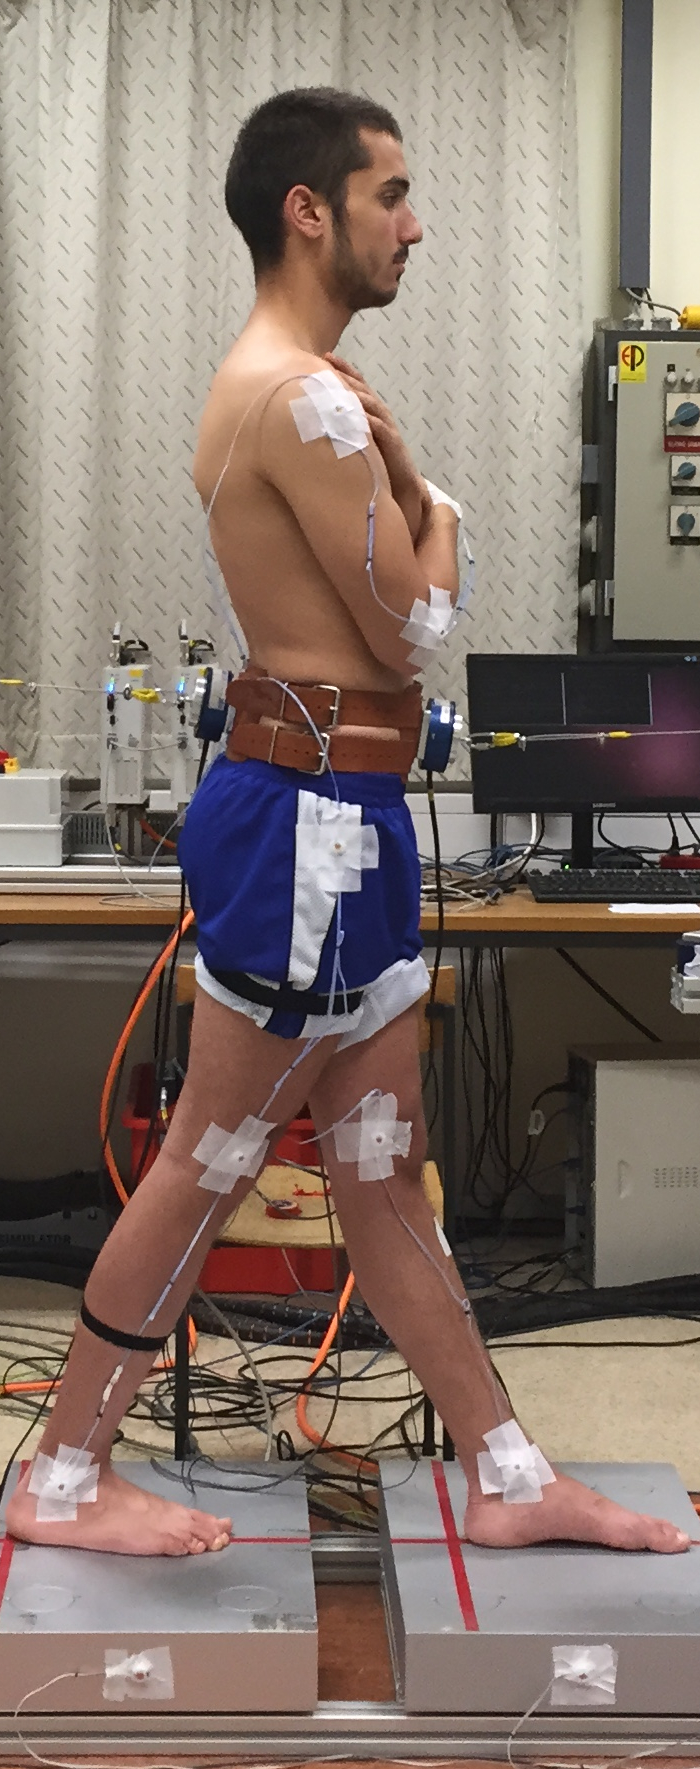
\includegraphics[width=0.2\columnwidth]{Morteza/figs/widestance.jpg} &
    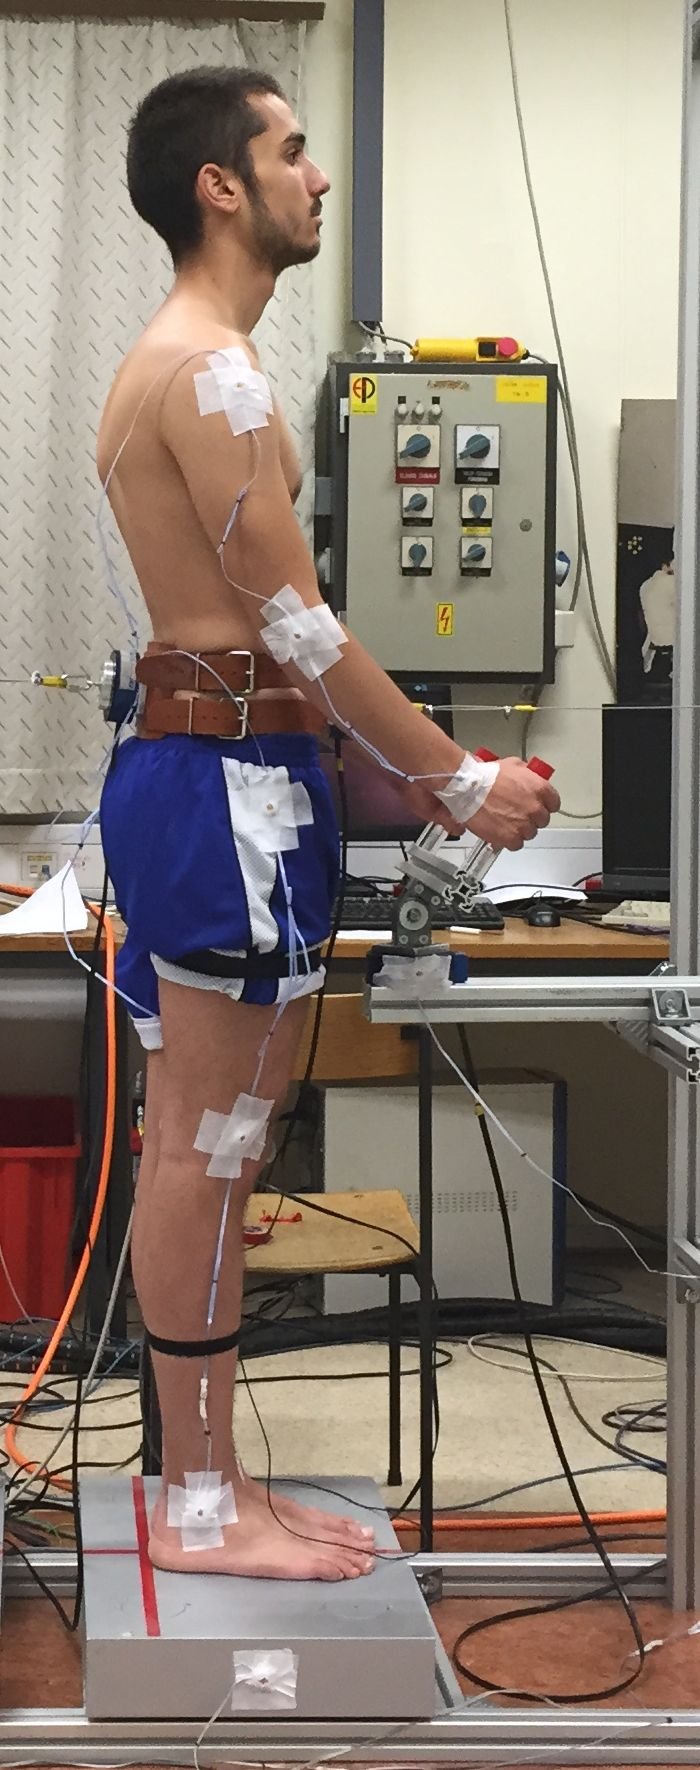
\includegraphics[width=0.2\columnwidth]{Morteza/figs/low.jpg} &
    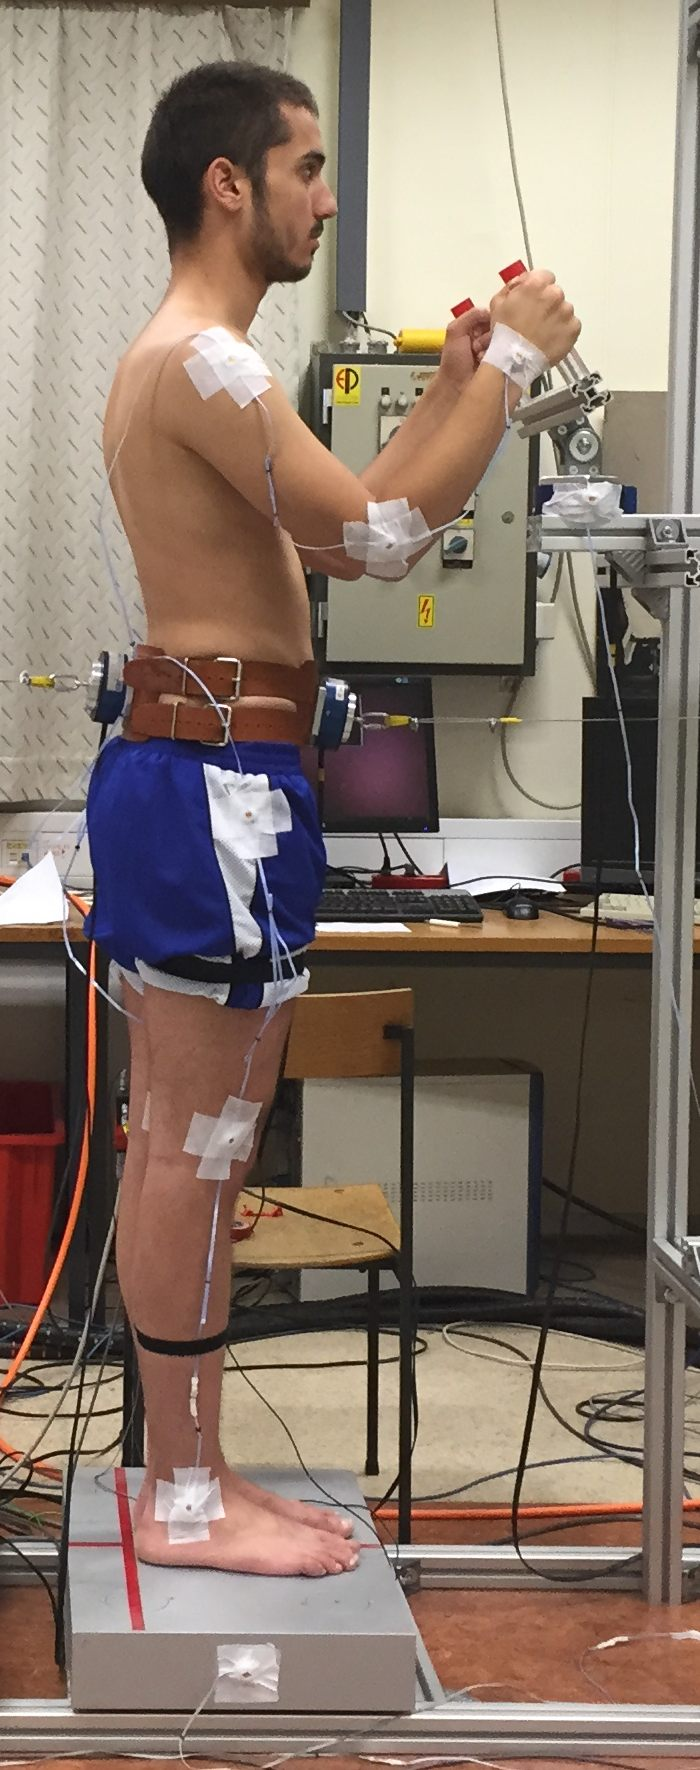
\includegraphics[width=0.2\columnwidth]{Morteza/figs/mid.jpg} &
    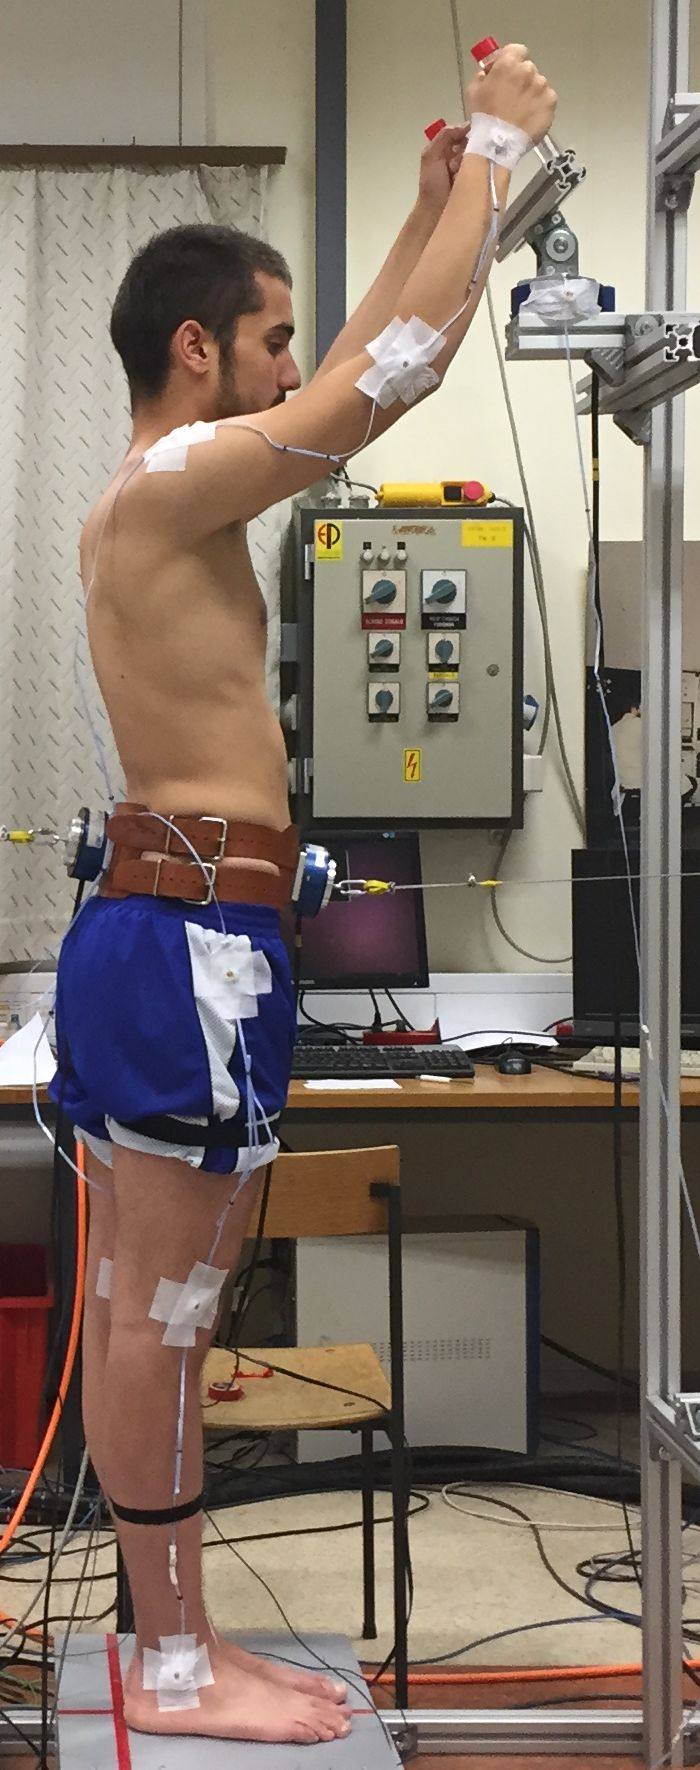
\includegraphics[width=0.2\columnwidth]{Morteza/figs/high.jpg} \\
    (b) & (c) & (d) & (e)
  \end{tabular}
  \caption{Experiments setup for five different positions: (a) stance, (b)
    wide stance, (c) low handle, (d) middle handle and (d) high handle.  A
    pulley mechanism, which is connected to the subject by a belt, perturbs
    the subject's CoM. Contact forces are measured at the feet and hands.
    Motion is recorded with an optical motion capture system.}
  \label{experimentsetup}
\end{figure}


\subsection{Methods}

\subsubsection{Subjects}

Eleven healthy male subjects participated in this study.  Their average age
was $21.7$ years (SD $=2.2$ years), height = $183$ cm (SD $=4.6$ cm) and body
mass $76.8$ kg (SD $=8.1$ kg).  The subjects were informed about the course of
the study prior to their participation and were required to sign an informed
consent approved by the National Medical Ethics Committee (No. 112/06/13).


\subsubsection{Measurement Protocol}

We observed the subject’s reactions to the external perturbations in five
different poses.  In the first pose (\textit{stance}), subjects were standing
straight with their feet together and arms crossed over the torso
(Fig.~\ref{experimentsetup}.a).  In the second pose (\textit{wide stance}),
subjects were standing with their arms crossed over the torso and their left
foot $60$ cm ahead of their right foot (ankle to ankle distance).  In the
third pose (\textit{low handle}), subjects were standing as in the first pose
and holding the handle which was located in front of their bodies at the hip
height (Fig.~\ref{experimentsetup}.b).  In the fourth pose (\textit{middle
  handle}), subjects were standing as in the first pose and holding the handle
which was located in front of their bodies at the shoulder height
(Fig.~\ref{experimentsetup}.c).  In the last pose (\textit{high handle}),
subjects were standing as in the first pose and holding the handle which was
located in front of their bodies and above the head
(Fig.~\ref{experimentsetup}.d).

The subjects were perturbed by a horizontal external force produced by our
force-controlled pulling mechanism \cite{Peternel&Babic13} at the approximate
position of their CoM \cite{Gardetal04}.  The command signal was a step with
$0.5$ second width (see Fig.~\ref{perturbations}).  The actual perturbation
force was controlled by a combination of a feed-forward and a PID feedback
controller.  We selected eight linearly increasing magnitudes of perturbation
forces where the maximum was defined as 22\% of the individual subject's body
weight and the minimum was $1/8$ of the maximum force (increasing rate of
$1/8$ of the maximum).  Between each perturbation we induced a random pause.
For each pose, we repeated the series of eight perturbations ten times (80
trials per subject per pose) and observed the human reactions.  We gave the
subjects 10 minutes pause between each pose.  In case of the first pose, the
subjects had to step before the maximum perturbation was reached.  When the
subject made a step, the experimenter stopped the procedure and moved to the
next series of perturbations.  The step was not required in other poses and
the series of perturbations repeated uninterrupted.
\begin{figure}
  \centering
  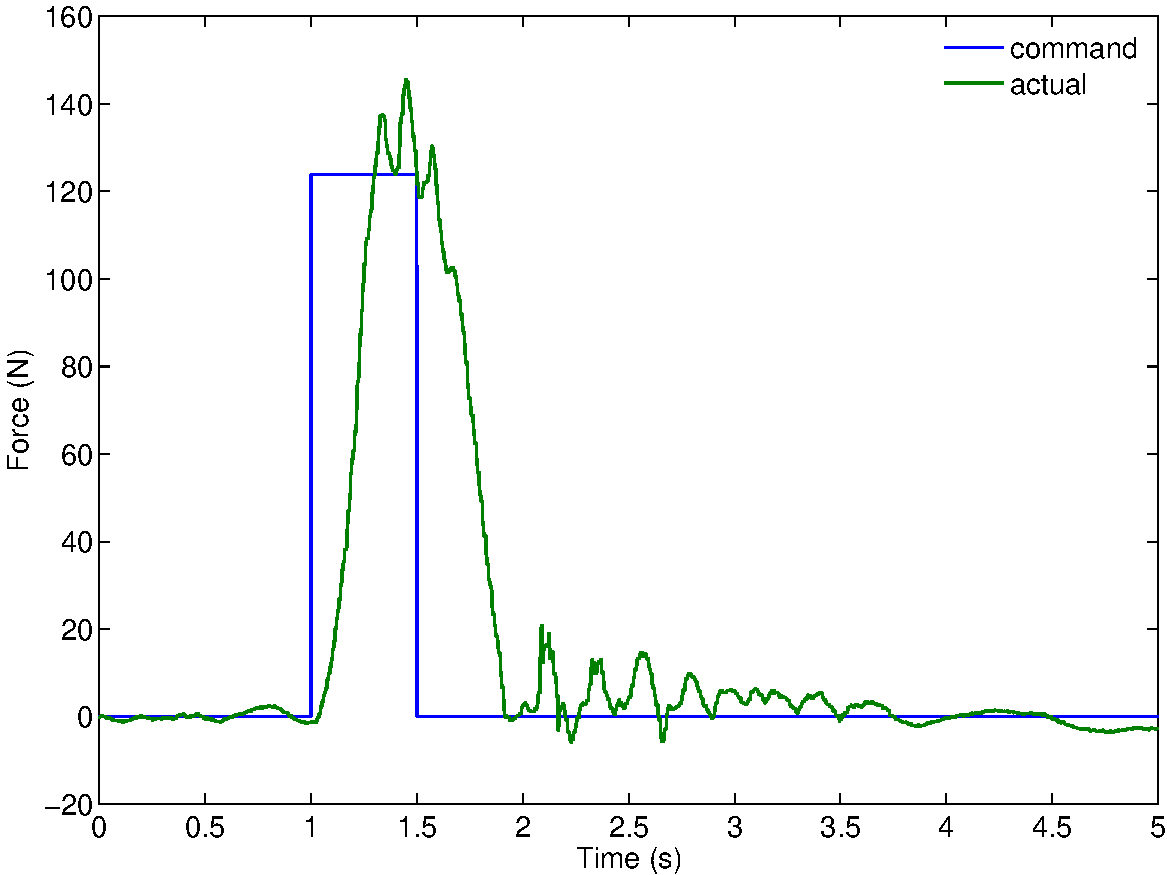
\includegraphics[scale=0.4]{Morteza/figs/perturbation.pdf}
  \caption{An example of the perturbation force applied to the CoM of the
    subjects.  This is for the subject whose body mass is $76.5$ kg.  The
    intensity of the perturbation is number $6$ meaning that the force is
    $6/8$ of the maximum for this subject.}
  \label{perturbations}
\end{figure}

Body movements were measured by a motion capture system (3D
Investigator$^{\tt\small TM}$ Motion Capture System, NDI, Waterloo, Ontario).
The optical markers were placed on the ankle, knee, hip, shoulder, elbow and
wrist.  The positions of the markers are used to calculate the joint angles.
We used two force plates (9281CA, Kistler Instrument AG, Winterthur,
Switzerland) to measure the ground reaction forces and center of pressure
position.  The handle was mounted on a 3-axis force sensor (45E15A, JR3,
Woodland, USA) to measure the force between the handle and the subject.

In order to estimate the starting time of the subjects' reactions, we measured
muscle activation in Triceps Brachii, Soleus and Tibialis Anterior by surface
electromyography (EMG).  We placed surface EMG electrodes (SX230 EMG sensor,
Biometrics Ltd, Newport, UK) on the selected muscles in accordance with SENIAM
recommendations \cite{Hermensetal99}.  We also placed a monitor in front of
the subject to provide visual feedback on the CoP position that allowed him to
move back to the initial pose after each perturbation.


\subsection{Model}

In the experiments, in order to produce movements which are planar only, we
prevented applying out-of-plane forces/moments to the subjects by providing a
pair of handles for them and perturbing them in a plane.  Therefore, we could
use planar models for both inverse dynamics and CoM manipulability
calculations.  Although, using a planar model for wide stance pose is a bit
unrealistic.  Planar humanoid models that we used for the stance, wide stance
and all three handle poses are shown in Fig.~\ref{planarhumanoids}.  These
models consist of multiple links which are connected to each other by actuated
revolute joints.  Note that lower legs are connected to the ground.  This is
because we assume that the feet of the subjects do not move during the
experiments.  To model the stance pose, we lock the DoF of the arms.  So, in
this case, the model has 3 DoF and is unconstrained.  For the wide stance, the
robot has 6 DoF and is constrained due to the kinematic loop in the legs.  For
the handle poses, the robot has five actuated DoF and it is constrained at the
hand to model the handle contact.
\begin{figure}
  \centering 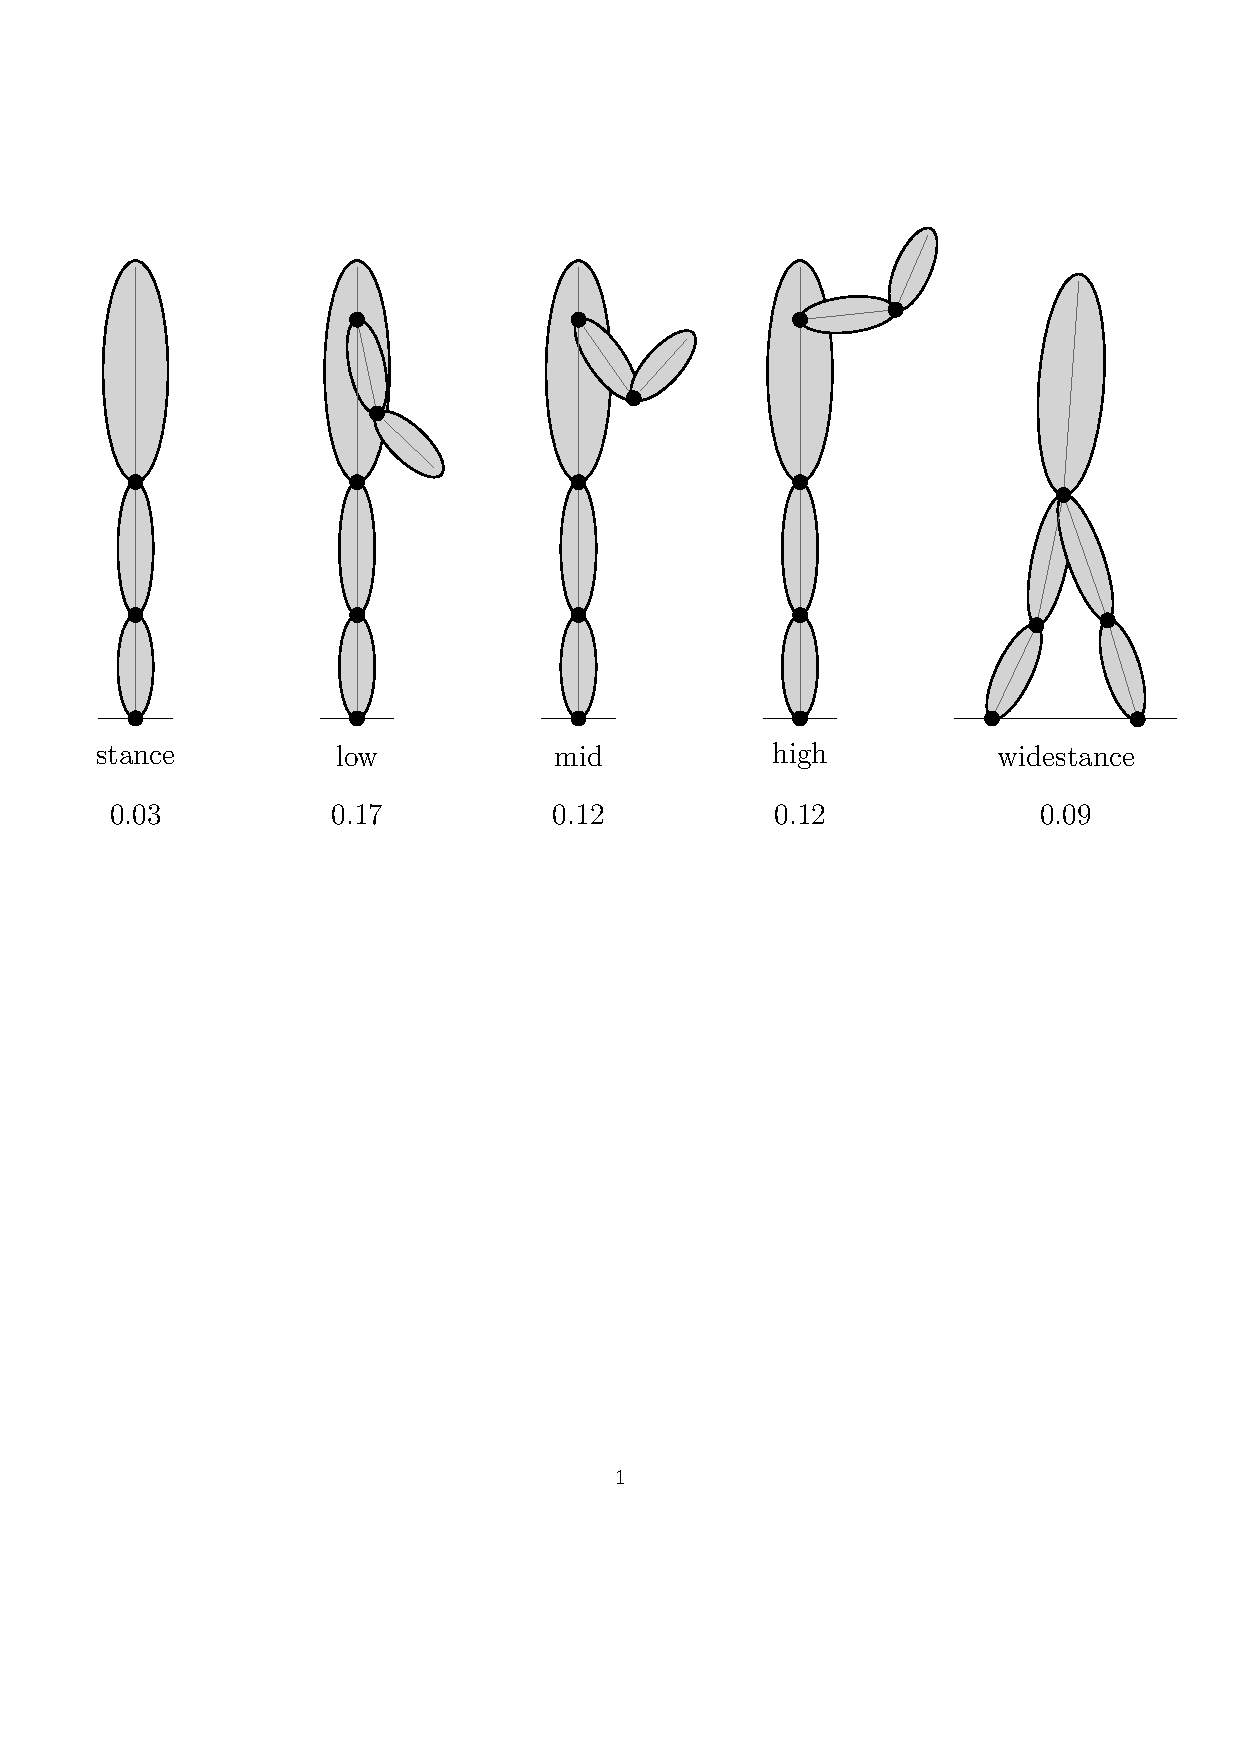
\includegraphics[trim = 13mm 154mm 10mm 37mm, clip,
    scale=0.85]{Morteza/figs/robotmodels}
  \caption{Schematic diagram of the planar humanoid robot model}
  \label{planarhumanoids}
\end{figure}

Since for balancing we are only interested in movements in the horizontal
direction, we calculate the maximum value of $\Delta \dot{\Bc}$ in this
direction for all five positions.  This represents the maximum achievable
change of velocity of the CoM in the horizontal direction and is a measure for
the ability to accelerate the CoM in order to correct its position in this
direction.  Due to the joint limits of the knees, instead of using
(\ref{torqueellipse}), we use the method that is described in
\ref{subsec:limits}.  Joint angles of the arms for the handle positions are
set to the average initial joint angles of the subjects that we calculate from
the marker positions.  For the low handle, the shoulder angle (angle between
torso and upper arm) is $12^\circ$ and the elbow angle (between upper and
lower arms) is $145^\circ$.  Shoulder and elbow angles are $35^\circ$ and
$77^\circ$ for the middle handle, and $96^\circ$ and $118^\circ$ for the high
handle positions, respectively.  For the wide stance position, we assume zero
angles in the knees and upright torso.  The weighting matrix that we use for
the calculations is a diagonal matrix as
%
\begin{equation}
  \BW = diag([2.33, 3.45, 4.55, 1, 1.25]) \, ,
\end{equation}
%
which is determined to include the differences in the joint's strengths
\cite{Anderson2007, Bober2002, Gandevia1998, Moraux2013}.

Calculated values for the maximum $\Delta \dot{\Bc}$ for the five positions
are mentioned in Fig.~\ref{planarhumanoids}.  As it can be seen in this
figure, the low position has the highest value (i.e. $0.17$) for the
manipulability and the stance position has the lowest one (i.e. $0.03$).
Manipulability for the middle and high positions are the same ($0.12$) and
lower than the low position.  Also wide stance manipulability (i.e. $0.09$) is
only better than the stance position.  Therefore, according to the
manipulability analysis for our models, we expect the same ranking for the
five positions in the sense of total average required torque to keep the
balance.  We will verify this hypothesis in the next subsection.


\subsection{Results}

As already mentioned, inverse dynamics are used to compute the torques that
are applied (at the joints) by the human subjects.  Joint angles are
calculated by using marker positions, and joint velocities and accelerations
are estimated by using simple time differentiation.  Lengths and inertial
parameters of the subjects are calculated via the software that is introduced
in \cite{Zlajpah&Babic14}.  Feather stone's Spatial software package
\cite{Featherstone} is used for the dynamics calculations.

To work out the average total torque for each position and each perturbation
intensity, first we calculate the joint torques from inverse dynamics for each
trial (in total $4400$ trials $= 5$ poses $\times 8$ intensities $\times 10$
reps $\times 11$ subjects).  Then we calculate the average torque over the
reps for each joint.  Note that, since maximum achievable torque of the arm
joints vary with arm configuration, we normalize shoulder and elbow torques
for the handle positions \cite{Anderson2007, Bober2002, Gandevia1998,
  Moraux2013}.  Then, we sum up the normalized joint torques to get $440$
(i.e. $5$ poses $\times 8$ intensities $\times 11$ subjects) values for the
average normalized joint torques.  The beginning time is the subjects' average
initial reaction time which is estimated by the average EMG signal.  The end
time is roughly the time that the subjects have recovered from the
perturbations.

%The same process gives us the average joint works.  The work is in fact the
%sum of $|\Btau \dot{\Bq}| \Delta t$, where $\Delta t$ is the data gathering
%frequency which is 2 milliseconds in our experiments.  We take the sum from
%$t=1.2$ s to $t=3$ s.

%% The values of the calculated normalized joint torques for the five positions
%% and different perturbation intensities are shown in
%% Fig.~\ref{jointtorquesubjects} for all subjects.  These values are marked by
%% $+$ In The graphs.  The Lines in the graphs are fitted to the values by using
%% least squares method.  Note that the graph of the first subject does not
%% include the results for high handle position.  This is due to the problem in
%% data gathering during the experiment which is solved for the next subjects.
%% \begin{figure}
%%   \centering
%%   \begin{tabular}{cc}
%%     subject 1 & subject 2 \\
%%     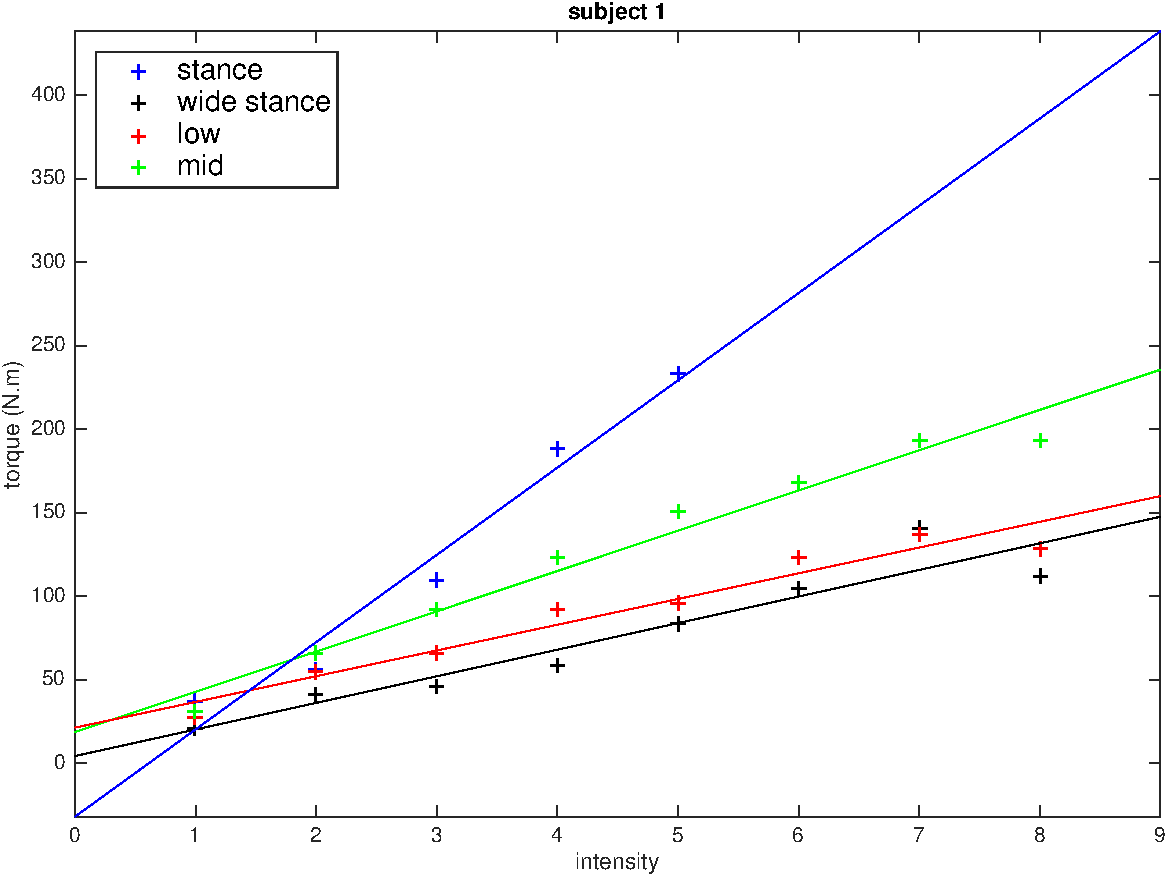
\includegraphics[width=0.46\linewidth]{Morteza/figs/subj1} &
%%     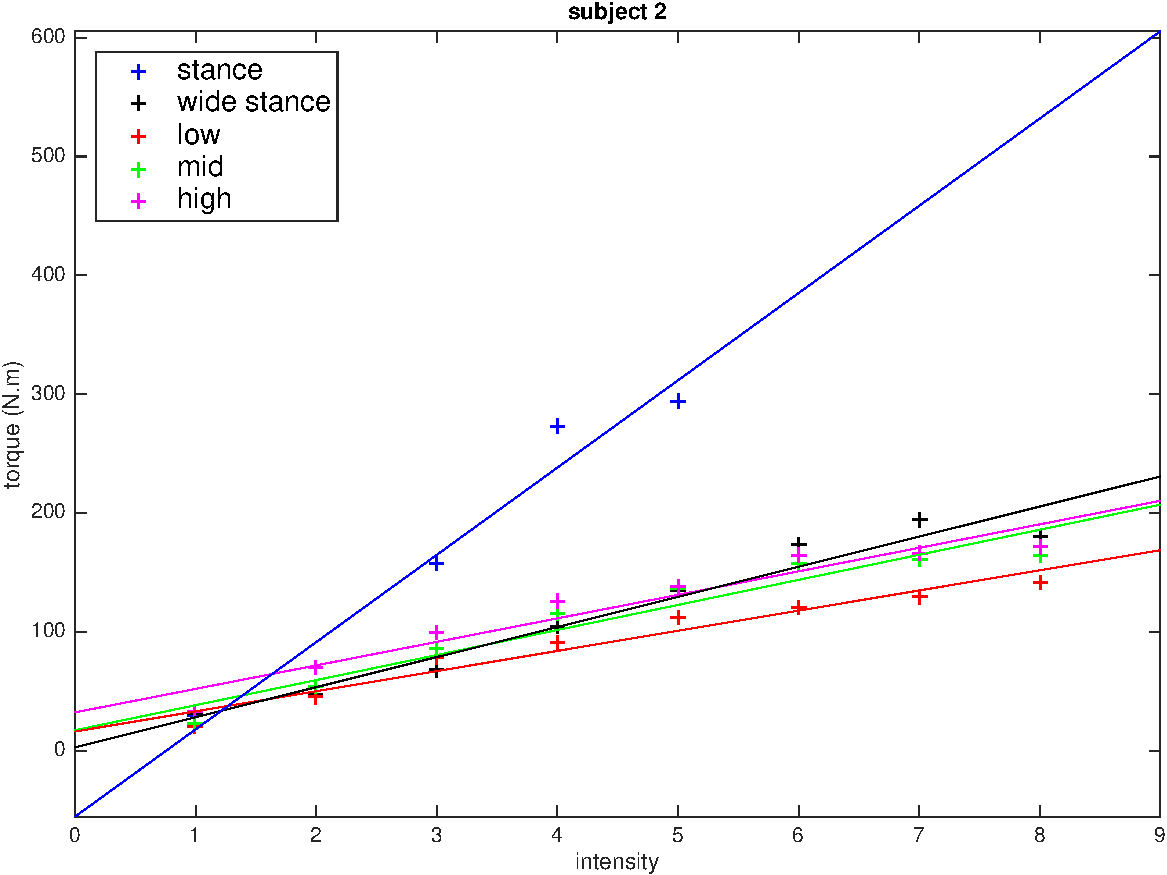
\includegraphics[width=0.46\linewidth]{Morteza/figs/subj2} \\
%%     subject 3 & subject 4 \\
%%     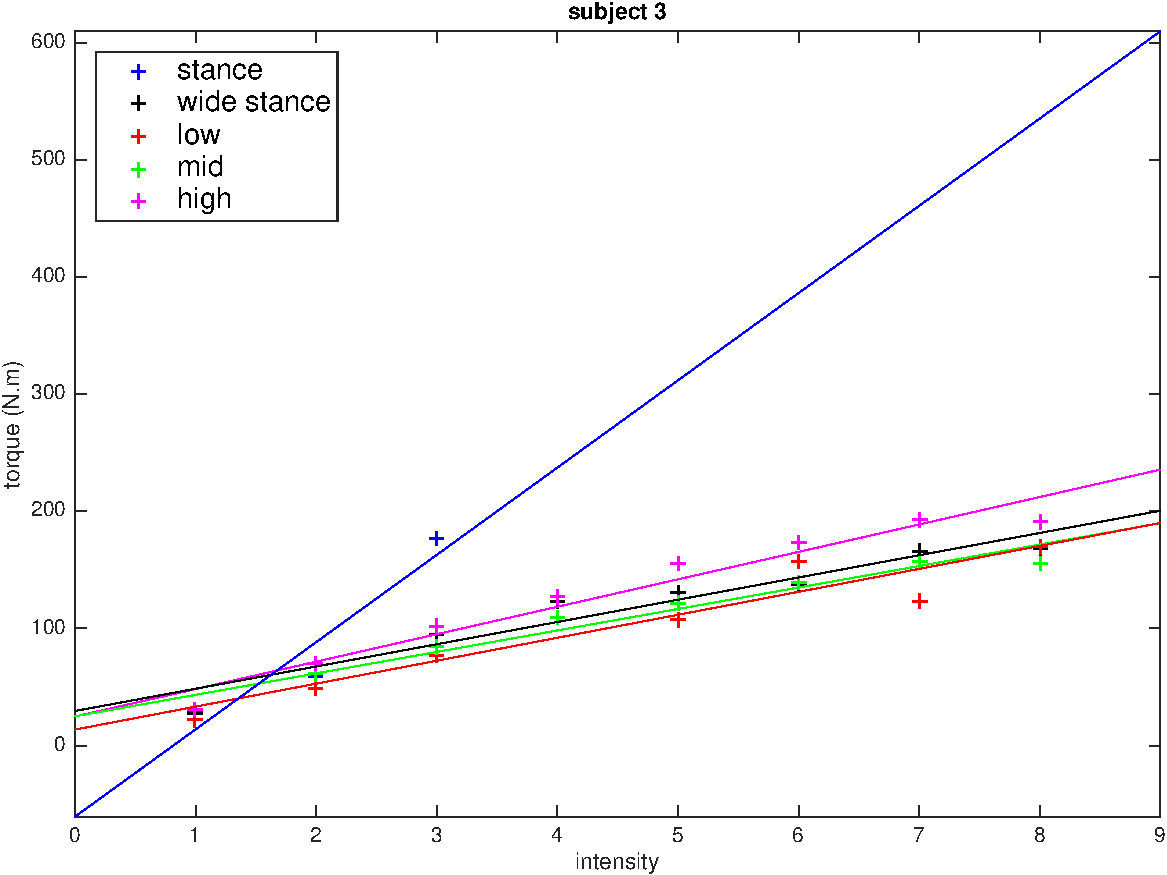
\includegraphics[width=0.46\linewidth]{Morteza/figs/subj3} &
%%     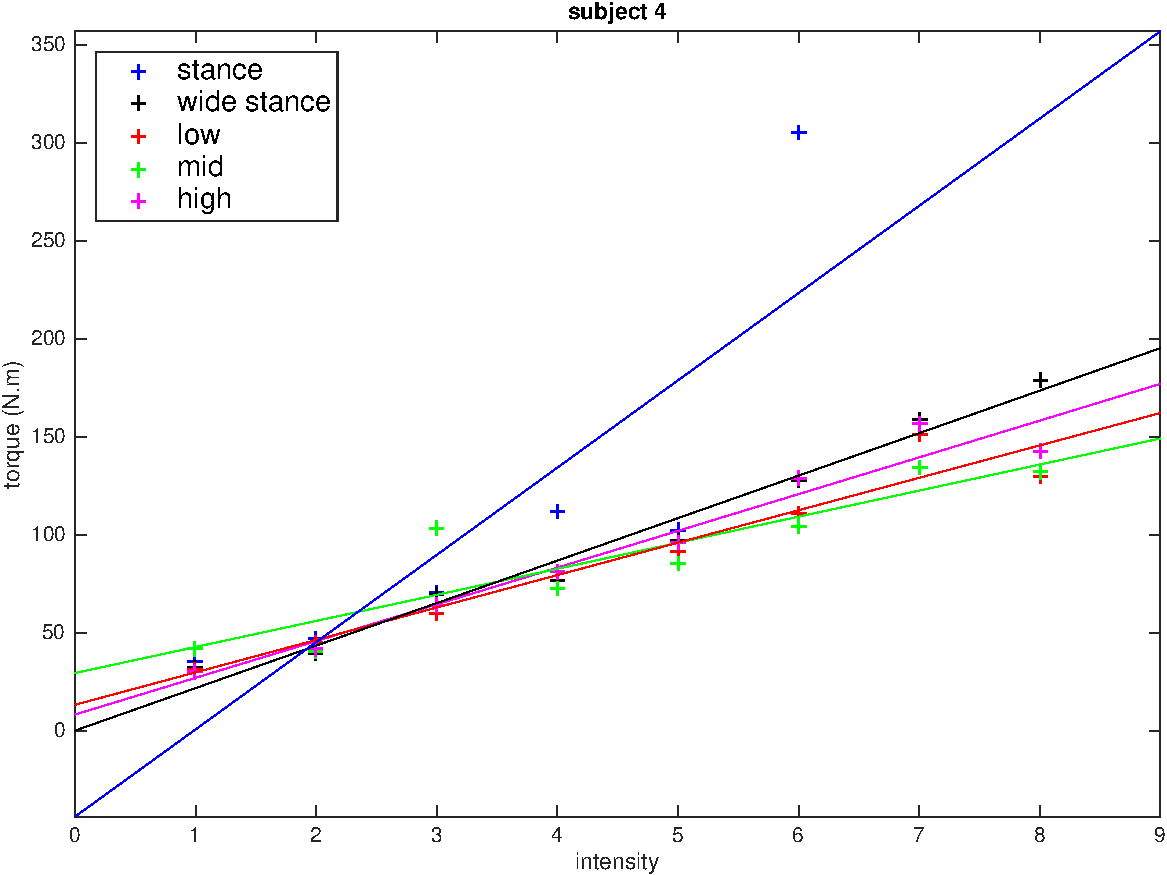
\includegraphics[width=0.46\linewidth]{Morteza/figs/subj4} \\
%%     subject 5 & subject 6 \\
%%     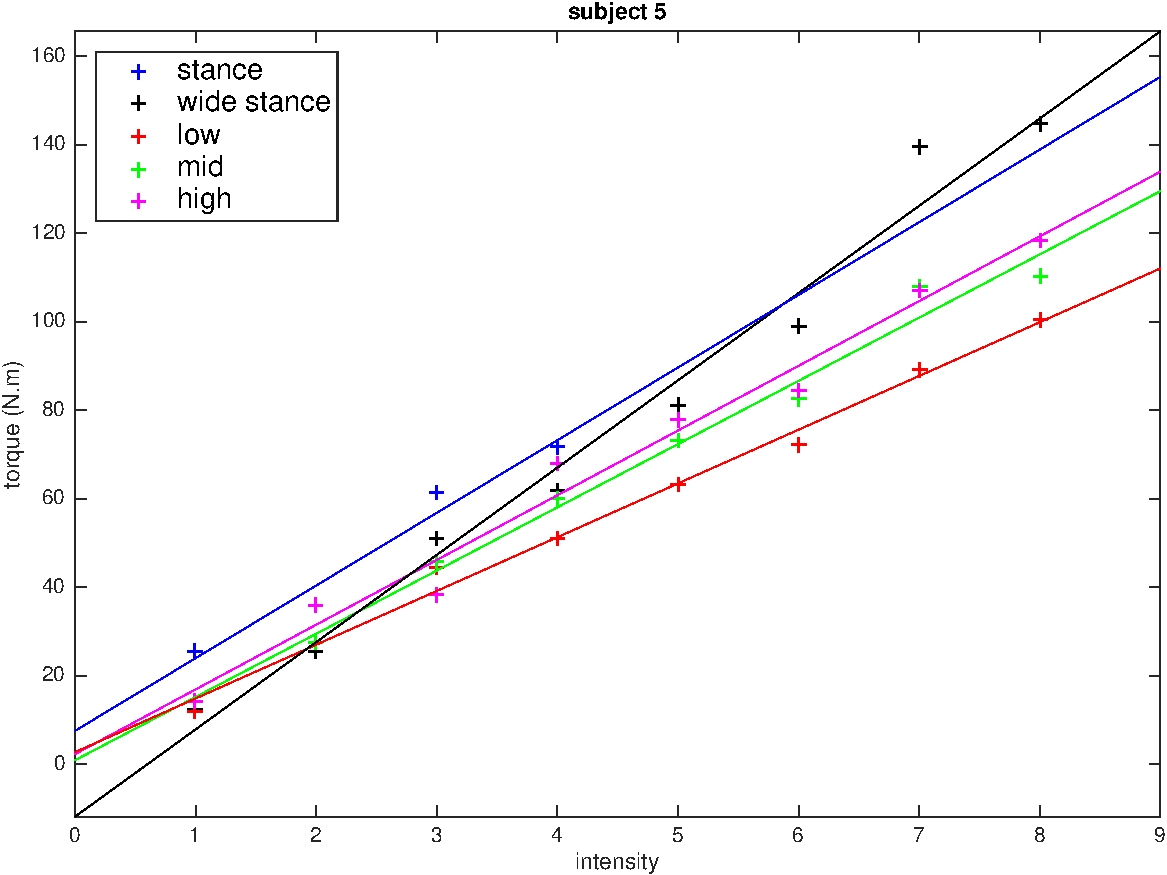
\includegraphics[width=0.46\linewidth]{Morteza/figs/subj5} &
%%     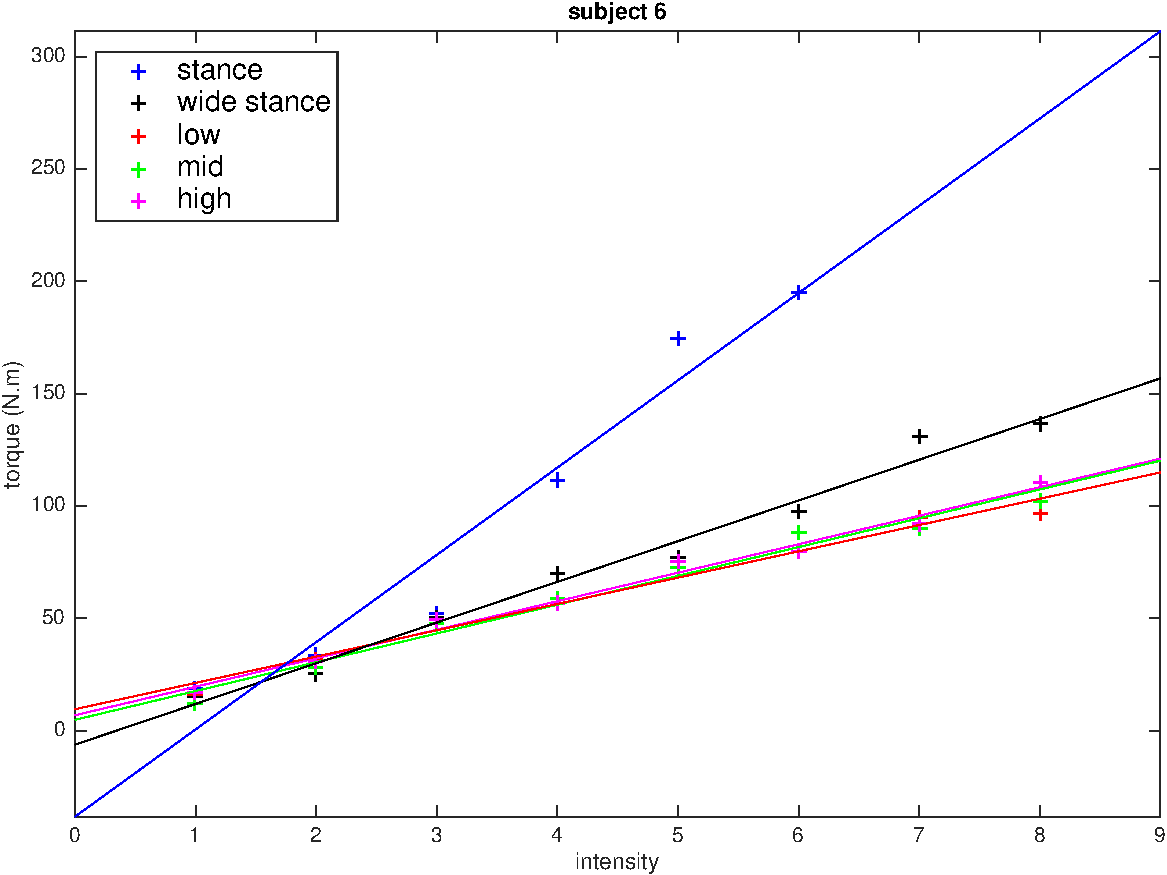
\includegraphics[width=0.46\linewidth]{Morteza/figs/subj6} \\
%%     subject 7 & subject 8 \\
%%     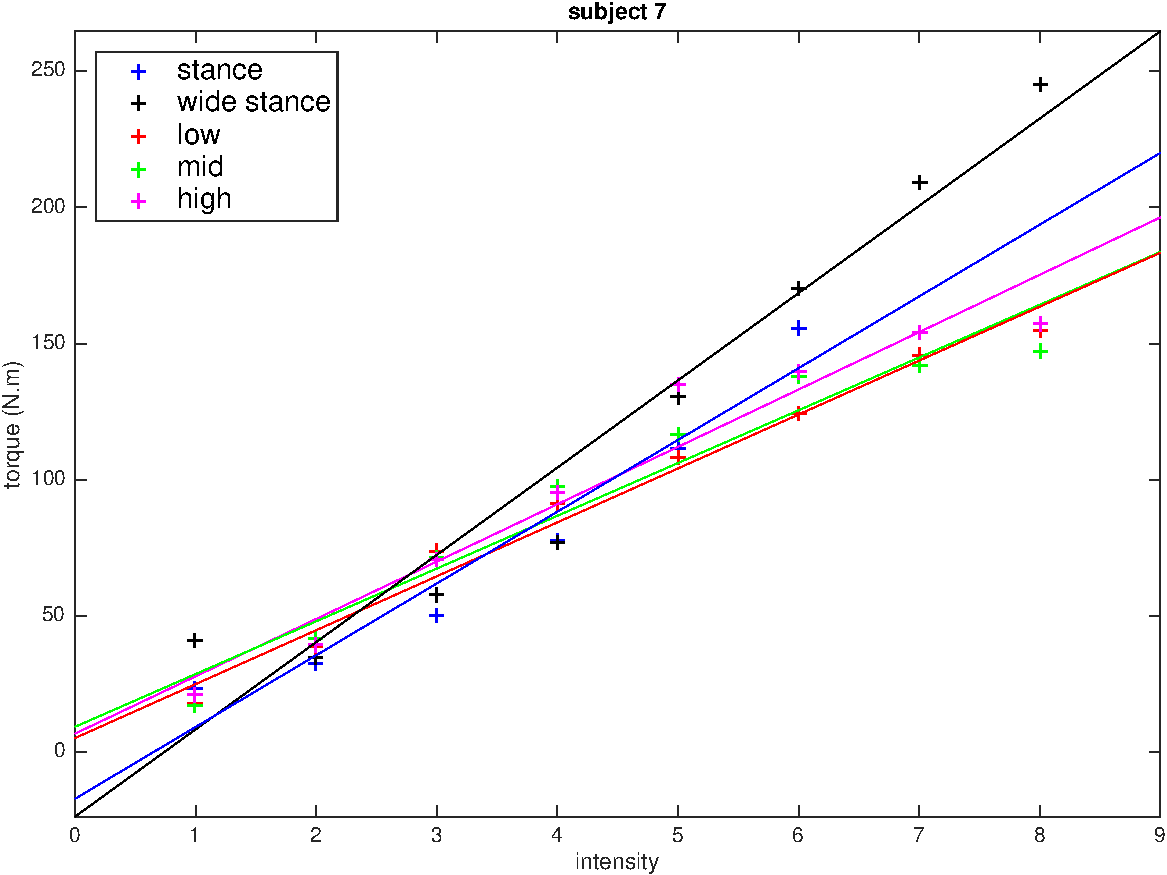
\includegraphics[width=0.46\linewidth]{Morteza/figs/subj7} &
%%     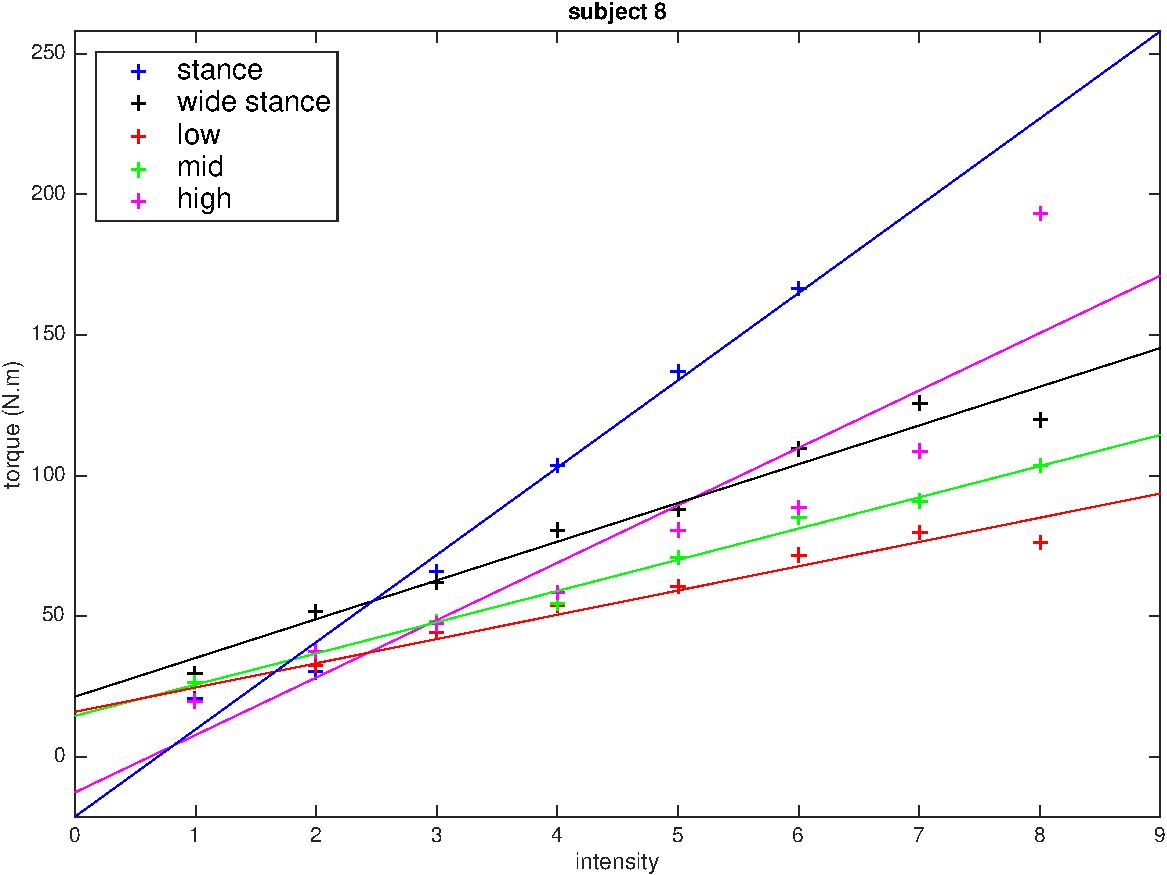
\includegraphics[width=0.46\linewidth]{Morteza/figs/subj8} \\
%%     subject 9 & subject 10 \\
%%     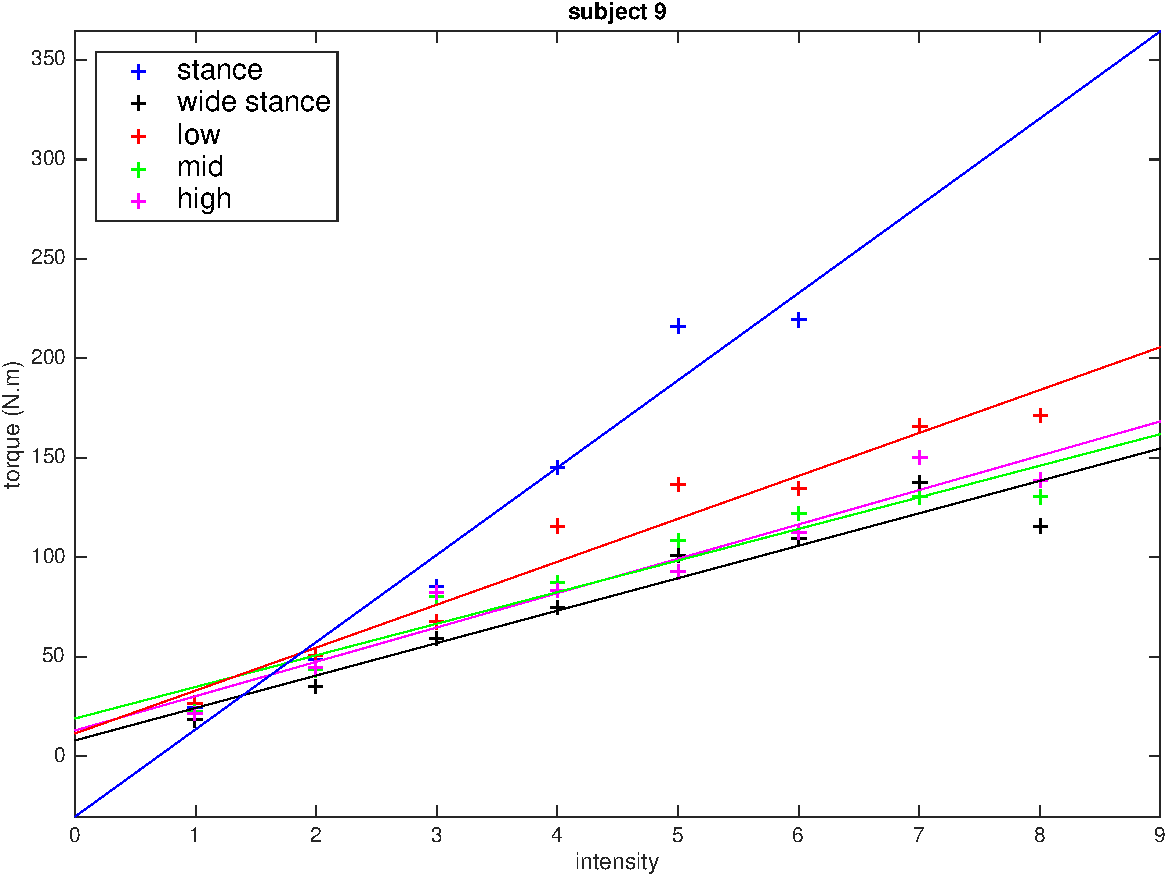
\includegraphics[width=0.46\linewidth]{Morteza/figs/subj9} &
%%     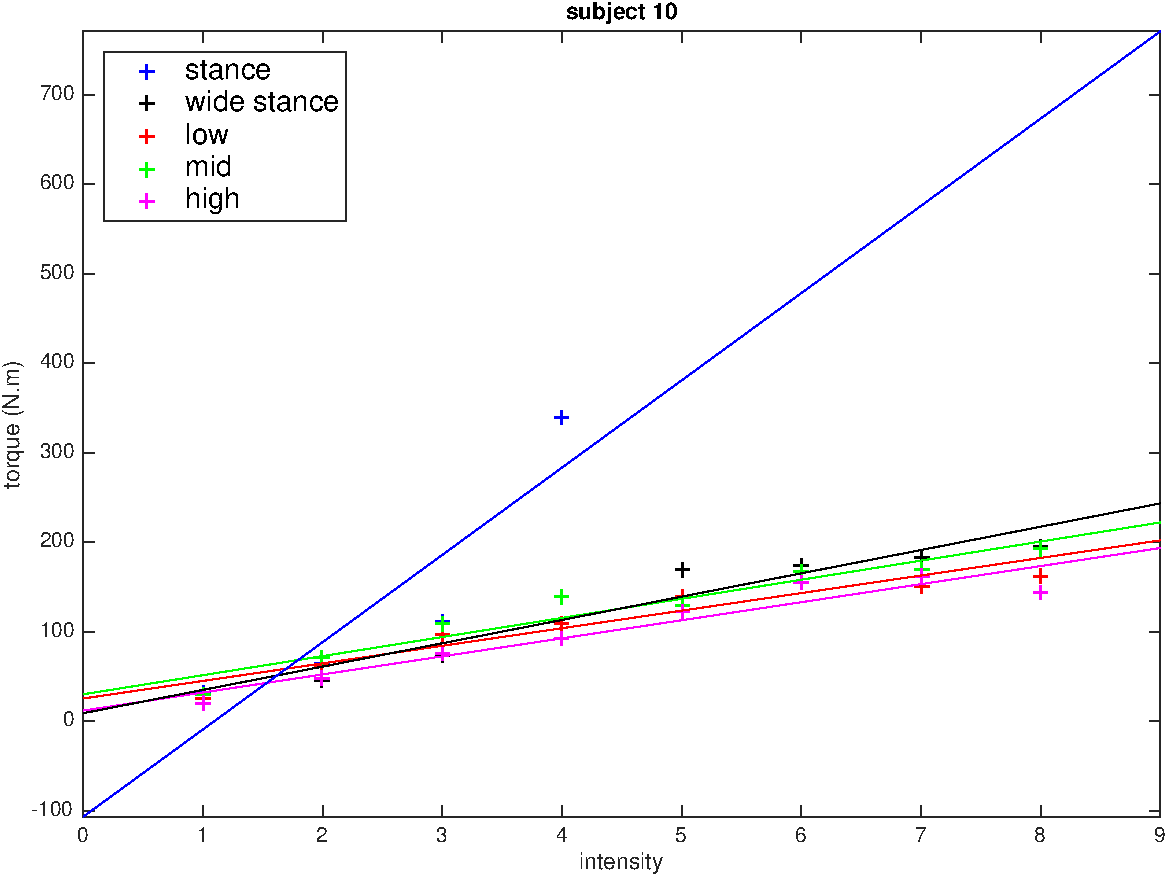
\includegraphics[width=0.46\linewidth]{Morteza/figs/subj10} \\
%%   \end{tabular}
%%   \caption{Total average normalized joint torques for the subjects at
%%     different perturbation magnitudes and different poses: stance (blue), low
%%     handle (red), middle handle (green) and high handle (magenta).}
%%   \label{jointtorquesubjects}
%% \end{figure}

The means of the normalized joint torques (per subjects) is shown in
Fig.~\ref{jointtorque}.  This figure shows the total average torque (after
removing outliers) for all subjects at each configuration and each intensity.
The lines are fitted to the values by using least squares method.  The
standard error of the means are also shown in this figure.  As can be seen in
this figure, the low handle pose has the lowest total torque and the stance
pose has the highest.  According to this graph, the ranking between the
positions is 1) low, 2) middle, 3) high, 4) wide stance and 5) stance.  This
ranking is more visible in higher intensities and it conforms with the
manipulability numbers from our analysis.  The only difference is that
manipulability analysis predicts that middle and high positions are the same
whereas experimental results show a bit difference between two (middle is
better than high).  Therefore, the experimental results agree with the
manipulability analysis in the previous subsection.  Configurations of greater
manipulability require less torque, in order to maintain balance after
perturbations of equivalent magnitudes.
\begin{figure}
  \centering 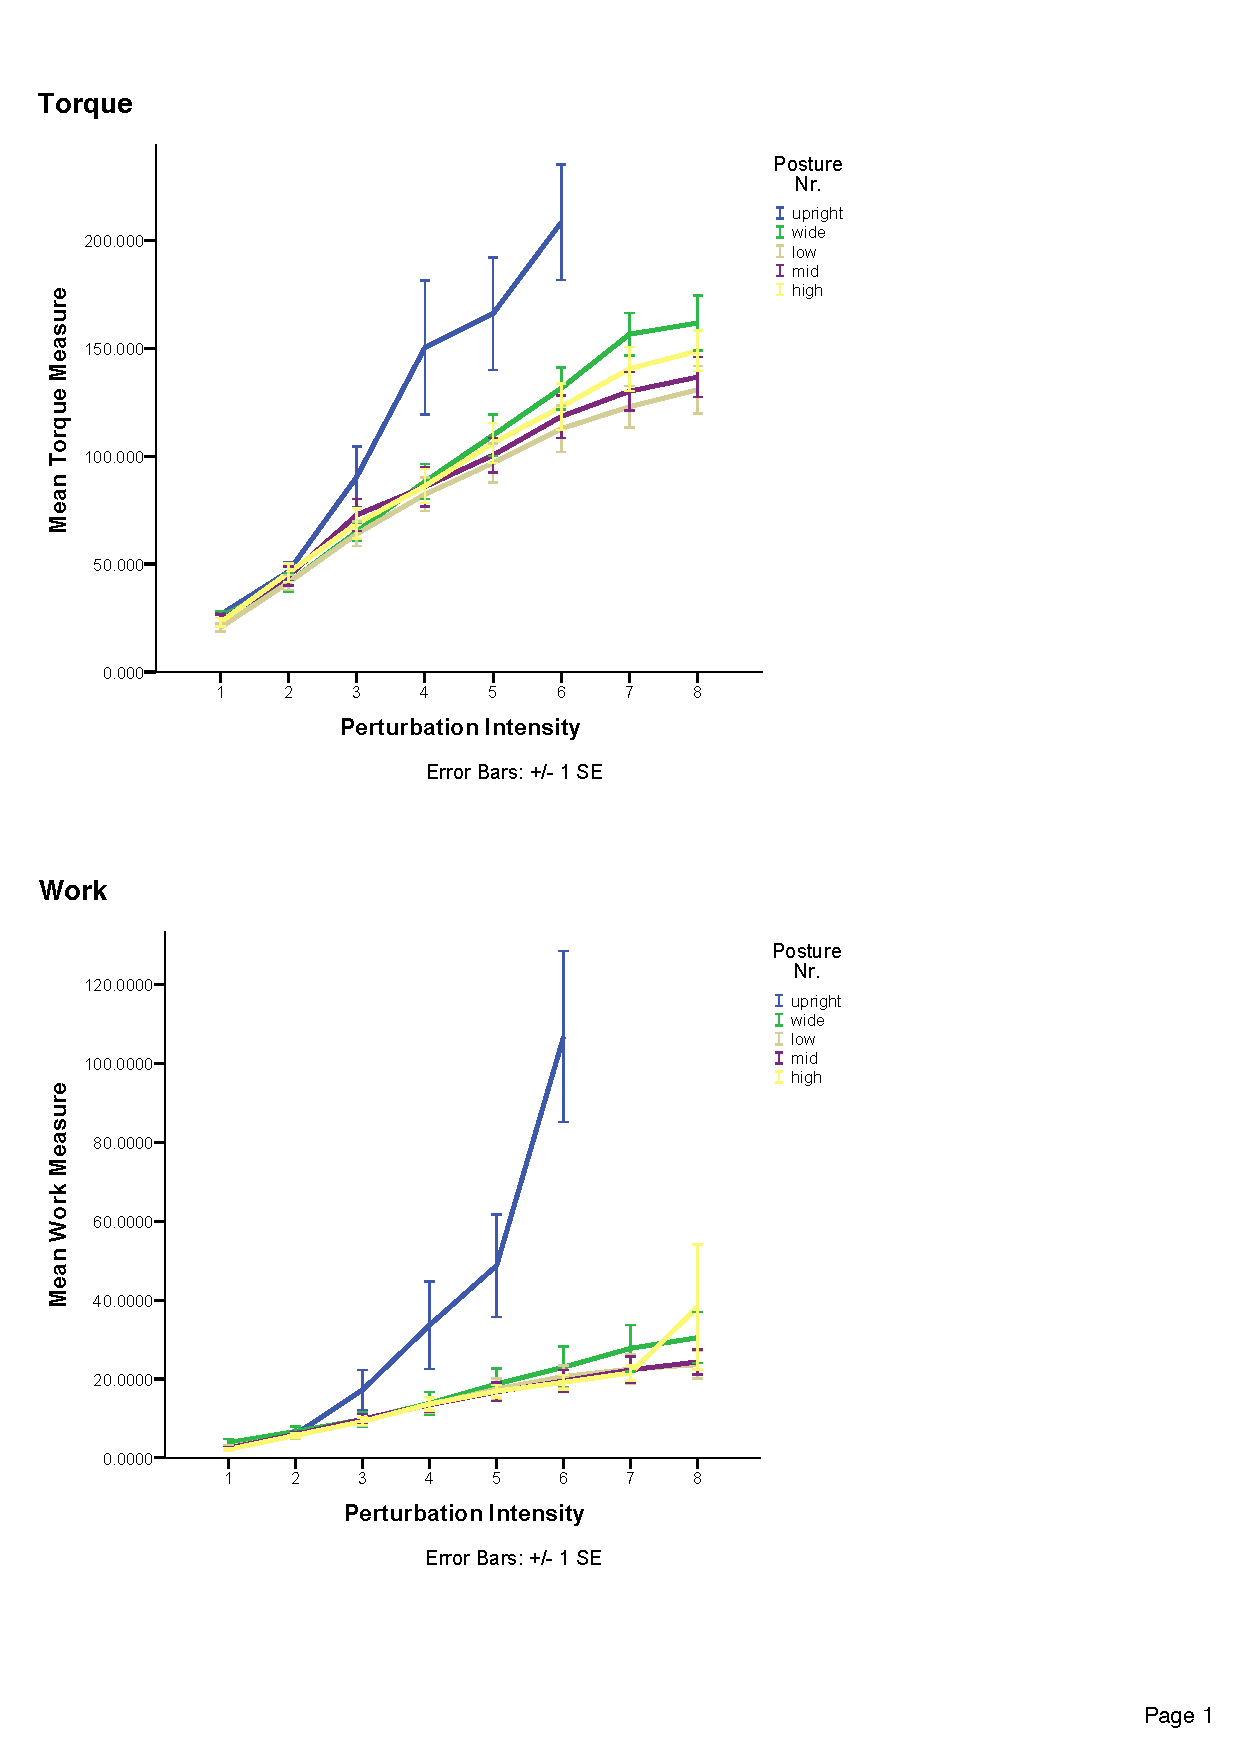
\includegraphics[trim = 1mm 150mm 10mm 10mm, clip, scale =
    0.95]{Morteza/figs/errorBarPlotsSEM-norm_v2}
  \caption{Average of the total torque for the subjects at each pose and each
    perturbation intensity.  The stance position required the most torque in
    order to maintain balance.  While the low handle position required the
    least amount of torque for the same perturbation.}
  \label{jointtorque}
\end{figure}


\section{Conclusion} 
\label{sec:conclusion}

A set of metrics are introduced in this chapter to study, analyse and measure
the ability to balance for humans and robots.  These metrics, which are called
the manipulability of the center of mass, provide two types of ellipsoids
which graphically show how the CoM can be accelerated in 3D space by a certain
amount of change of motion (due to impulses) at the joint space.  These
ellipsoids can be used to measure torque efficiency and maneuverability of
humans and robots.  The proposed metrics are applicable to floating base
robots with non-breakable contacts with the environment.  Also, experiments on
human subjects are performed to investigate the applicability of the proposed
metrics for human studies.  In the experiments, the standing subjects (in five
different configurations) were perturbed by a controlled force acting on their
CoM.  Then, the selected configurations were ranked according to the average
total torque that is applied by the subjects to recover their balance at each
configuration.  It is shown that the proposed metric for torque efficiency can
successfully predict the same ranking between the configurations as the
experimental results suggested.  This agreement shows the applicability of the
metrics for human studies as well.  Therefore, manipulability of the center of
mass provides greater insight into the posture controllability of humans and
robots, in various configurations and contact conditions.


%% \section*{ACKNOWLEDGMENT}

%% The work presented in this paper is supported by the European Community
%% Framework Programme 7 through the CoDyCo project, contract no. 600716.






\chapter{Postural Control Precedes and Predicts Volitional Motor Control}\label{sec:ElmarPrePrint}


Supportive hand contacts are essential for mastering every-day life tasks, for 
example, when reaching for a glass on the highest shelf humans typically have to 
use the other hand to support their body on the kitchen table. In such 
scenarios, the motion of the body and both arms have to be perfectly 
synchronized to successfully perform the reaching motion and to simultaneously 
ensure the postural stability. However, little is known about the underlying 
processes that govern the motion of the human body during and after the learning 
of these kinds of concurrent motor skills. To study the effect of supportive 
contacts on motor control of reaching, an innovative full-body experimental 
paradigm was established that extends current experimental methods to a more 
ecological setting. The task of the subjects was to reach with their right arm 
for a distant target on a screen while postural stability could only be 
maintained by establishing an additional supportive hand contact with their left 
arm. To examine adaptation, non-trivial postural perturbations of the subjects' 
support base were systematically introduced. A novel probabilistic trajectory 
model approach was employed to analyze the correlation between the motions of 
both arms. We found that subjects adapted to the perturbations by establishing 
supportive hand contacts that were dependent on the location of the reaching 
target. Moreover we found that the trunk motion adapted significantly faster 
than the motion of the arms. However, the most striking finding was that 
observations of the initial phase of the left arm or trunk motion (100-400 ms) 
were sufficient to faithfully predict the complete movement of the right arm. 
Overall, our results suggest that the goal-directed arm movements determine the 
supportive arm motions that ensure postural stability and that adaptation 
happens on different time scales, where the motion of heavy body parts adapts 
faster than light arms. 

\section{Introduction}
Most of our every day motor skills involve strict control of postural stability 
in parallel to the execution of the primary motor task. A great deal of these 
tasks also require additional supportive hand contacts beside the feet that are in contact with the ground. An example task is the reaching for a glass on 
the highest kitchen shelf when we typically have to use the other hand to 
support the body by leaning on the kitchen counter. To successfully perform such a reaching 
motion and to simultaneously ensure the postural stability, the motion of the 
body and both arms have to be perfectly synchronized and coordinated.

In general, supportive hand contacts increase the stability during balancing and 
complement humans' sophisticated motor abilities, e.g., in reaching for distant 
objects, during acrobatics or simply to navigate in the dark through leaning 
against a wall\cite{cordo1982properties, jeka1994fingertip, 
balasubramaniam2002dynamics, dickstein2003effects}. 
%Balancing is known as the most basic motor control problem \cite{reed1982outline, Hofsten1993prospective}. 
Like the ability to balance, the utilization of supportive hand contacts has to be learned \cite{reed1982outline, Hofsten1993prospective}. 
At about two months infants are able to balance and turn their head to focus on 
interesting events; at six months they can balance in sitting position; at eight 
months infants already learn how to balance on hands and knees during crawling; 
at ten months they start walking with support from hanging on a table or a 
couch; and at about one year infants already know how to balance on two feet and 
walk independently across the room \cite{adolph2002learning, adolph2006motor}. 
While it is known that people develop optimal motor control strategies both for 
postural stability and manipulation \cite{pai1997center, scott2004optimal, 
todorov2004optimality}, it is unclear how these two distinctive motor tasks 
relate to each other and how their relationship affect the learning of novel motor 
skills or when re-establishing motor abilities in novel environments. A thorough 
understanding of these issues is of particular interest for the field of 
rehabilitation, where correlations between the primary motor tasks and the 
underlying supportive motor actions could be exploited in progress monitoring 
and novel pre-tests of motor dysfunctions \cite{duncan1990functional}. 

%Despite the obvious importance, little is known about the underlying motor 
%control processes that govern the motion the human body during and after 
%learning of these kind of concurrent motor skills. 

Many of previous studies 
either focus on control of postural stability \cite{horak1986central, 
kuo1995optimal, winter1995human, Lockhart2007}, study adaptation of arm reaching 
in confined lab environments \cite{shadmehr1993postural, wolpert1995arm, d2006control, 
diedrichsen2010coordination, berger2013differences}, or study situations when 
postural stability and arm reaching are only indirectly related 
\cite{flash1990human, stapley1999does, slijper2000effects, babivc2014effects, 
johannsen2007effects}.
%
In our study we propose an innovative full-body experimental paradigm 
(\FigureAbbr 
\ref{fig:subFigContactLocationsAllSubjects}A) that extends current experimental 
methods to a more ecological setting where postural stability and manipulation 
skills are tightly interrelated and interdependent to each other. We hypothesize that the arm reaching motions determine the supportive hand 
contact strategies and that both motor tasks adapt during training. In 
particular, we assume that these two motor tasks are correlated which is 
reflected in synchronized motor executions and a significant correlation between 
target locations and supportive hand contacts. To effectively elaborate on these hypotheses we designed an experimental paradigm where we
asked $20$ 
healthy subjects to reach with their right arm for a target displayed on a 
screen while using their left arm to maintain postural stability by leaning on a 
table in front of them.
Non-trivial postural perturbations 
of the subjects' support base were systematically introduced to examine 
adaptation and a novel probabilistic trajectory model approach was employed to 
analyze the correlations between the supportive arm motion and the motion of the 
arm to reach for the distant target.


\begin{figure}[t]
\centering
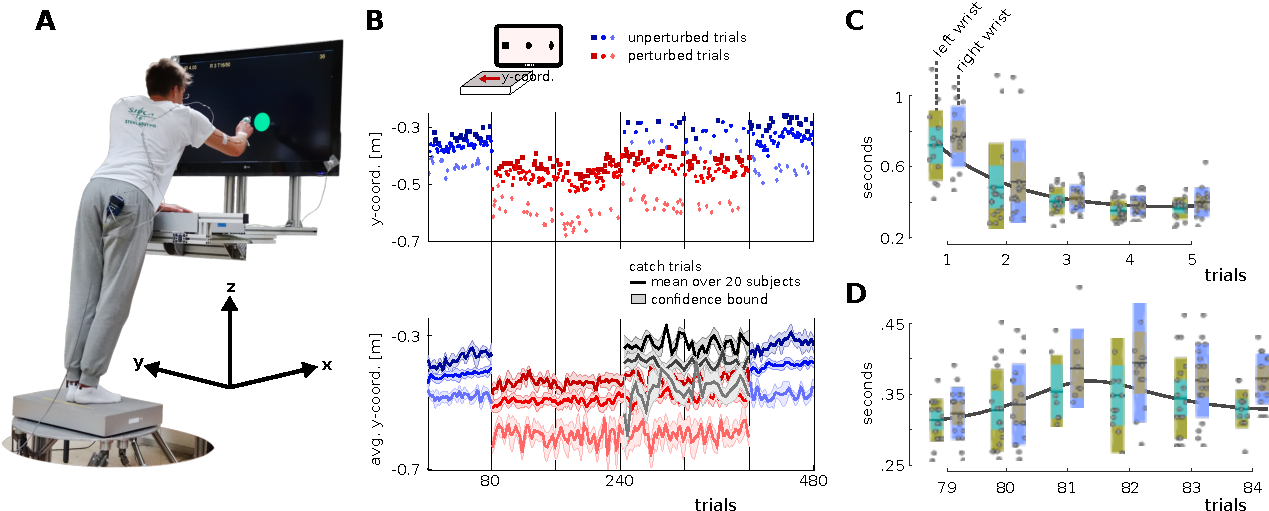
\includegraphics[width=\textwidth]{Elmar/picsClean/Fig1ExperimentContactsOnsets}
%\label{fig:subfig2}
 \caption{\textbf{Experiment, target dependent contacts and synchronized arm motions.} \textbf{A)} Experimental setting. 
 \textbf{B)}  The top row shows contact locations for a single representative subject 
 and the bottom row shows the mean and the confidence bound over all $20$ participants. 
 The first $80$ trials and the last $80$ trials are unperturbed sessions. 
 Catch trials were initiated during trials $240$ to $400$ and are denoted by the black lines in \textbf{B}.
%  
%  Note that during catch trials the contact 
%  location immediately switches back to the unperturbed behavior. This can be explained by the fact that the contact location 
%  is a result of both, the trunk motion (which shows strong negative after effects) and the left wrist motion (were we could not find these effects). 
%  Another finding is that contact locations are target correlated denoted by the three lines in \textbf{B} . 
 \textbf{C)} Illustration of the movement onsets of the wrists for the first five trials. 
 \textbf{D)} Movement onsets for the first six trials transitioning to the perturbed session. 
}
\label{fig:subFigContactLocationsAllSubjects}
\end{figure}


%NOTE Implications will be moved to the discussion 
\section{Results}%\label{sec:methods}

After a random interval of one to 
three seconds, the target was presented on the screen at one out of three possible locations (i.e., randomly at the left, the center or the right side on a horizontal bar). We motivated the subjects 
through a monetary reward that was proportional to the time needed to reach for 
the target. This reward was displayed after the target was reached. The number zero was displayed if the trial time exceeded two seconds. 
In our results, we focused on the y-coordinate of the contact locations 
as it corresponded to the direction of the translational 
perturbation. This is indicated by the arrow labeled by $y$ in \FigureAbbrP \ref{fig:subFigContactLocationsAllSubjects}. 

%\subsection*{Humans pick task dependent contact locations} 

\subsection{Subjects chose task dependent contact locations} 

Analysis of 
variance (ANOVA) showed a significant effect in the left hand contact location between 
sessions when the subjects were perturbed and unperturbed during reaching toward 
targets displayed on screen, $F(1,19) = 113.632$, $p < 0.001$, $\eta_p^2 = 0.857$.

The post-hoc analysis showed that the left hand contact location was significantly 
different between reaching toward all three distinctly positioned targets in 
perturbed, $t(19) = 6.85 \text{ to } 11.58$, $p < 0.001$, and in unperturbed trials, $t(19) = 
6.78-12.21$, $p < 0.001$.

There were also significant differences between means of contact locations for 
each target between perturbed and unperturbed trials (target one, $t(19) = 10.07$, $p 
< 0.001$, $d = 2.01$; target two, $t(19) = 10.22$, $p < 0.001$, $d = 2.38$; target three, $t(19) = 
11.51$, $p < 0.001$, $d = 3.25$), see Supplementary \FigureAbbr 
\ref{fig:SubFigANOVAContacts}.



%it is known that preparation actions depent on future actions cite Schack
%here we investigate is contacts change depdent on future goal-directed reaching

%We found distinct contact locations for each of the three tested targets during 
%the unperturbed cond. and the perturbed condition %Figxx (a-b)

%Subject frame reports numbers that are a result of both, trunk and left arm movements. 

Further, we analyzed individual sessions of unperturbed, perturbed and catch 
trials. We compared them with each other to determine whether there are any 
differences between contact locations and for which target positions they apply.

The first $80$ trials out of $480$ training trials were unperturbed. We found that 
there was a significant effect of target locations on the supportive contact 
locations in these first $80$ trials, $F(1.11,21.14) = 104.61$, $p < 0.001$, $\eta_p^2 = 
0.846$, see \FigureAbbr \ref{fig:subFigContactLocationsAllSubjects}B. Post-hoc tests using the Bonferroni correction \cite{bland2000introduction} revealed 
that there was significant difference in chosen supportive contact location 
between all three targets ($t(19) = 6.92 \text{ to } 11.66$, $p < 0.001$).

After the initial training phase, all subjects had to adapt to translational 
perturbations of the support base. Note that to compare the contact locations and the 
marker trajectories of perturbed and unperturbed trials, we corrected all sensor 
readings by the motion of the moving base. We refer to this correction as the 
\textit{subject frame}. Later we will introduce \textit{shoulder frames} to 
separate adaptation in the trunk and in the arms. Again, we found that there was a 
 significant effect of the target location on the contact location over all perturbed 
 trials, $F(1.33,25.27) = 116.39$, $p < 0.001$, $\eta_p^2 = 0.86$, see trials 
 $81 \text{ to } 240$ in \FigureAbbr \ref{fig:subFigContactLocationsAllSubjects}B. Post-hoc 
tests showed a significant difference in the chosen supportive contact location 
 among all three targets ($t(19) = 6.85 \text{ to } 11.58$, $p < 0.001$).

Consolidation of the postural control strategies was tested through randomly 
initiating unperturbed trials (catch trials). In the last phase of perturbed 
trials (trials $320$ to $400$), where adaptation can be assumed to be converged, 
the perturbation was deactivated for $30$ random catch trials. When comparing initial training 
trials with catch trials post-hoc tests showed no significant difference for all 
three targets, target one ($t(18) = -1.99$, $p = 0.062$, $d = -0.74$), target two 
($t(18) = -3.28$, $p = 0.004$, $d = -1$) and target three ($t(18) = -1.03$, $p = 
0.315$, $d = -0.39$).
%
Comparison of perturbed and catch trials showed significant differences in 
contact locations for all three target locations ($t(18) = -11.24 \text{ to } -12.97$, $p < 
0.001$, $d = -2.44 \text{ to } -1.93$).
%
For the washout, no significant difference was observed between contact 
locations for individual targets when comparing catch and final trials $401 \text{ to } 480$ 
($t(18) = -1.59 \text{ to } 1.28$, $p = 0.13 \text{ to } 0.22$, $d = -1 \text{ to } -0.39$).



%Conclusion 
In summary, we found that subjects chose distinct contact locations dependent on the 
target location on the screen. Catch trial tests revealed that the participants 
learned specialized control strategies for unperturbed and perturbed conditions. 
However, whether the distinct contacts result from trunk or left arm adaptations 
can not be answered from looking at contact locations only. That 
requires a more detailed analysis of the temporal profiles for which we will 
introduce a probabilistic trajectory model. 

%Implication


\subsection{Supportive and goal-directed movements synchronize}

Decreasing reaction times are an indicator for adaption of a pre-processing 
phase \cite{klatzky1995planning}. In line with this, we found that the movement onsets of the left 
and the right wrist synchronize within $3-5$ trials in the unperturbed training 
phase (left wrist: $323 \, \pm 44 \textrm{(SD)}$ ms, right wrist: $335 \, \pm 46$ ms) and when the 
perturbations are experienced for the first time (left wrist: $333 \, \pm 48$ ms, right wrist: $342 \, \pm 49$ ms). 
For the first six trials, the onsets of all subjects and the computed means and standard deviations (SD) are illustrated in \FigureAbbr \ref{fig:subFigContactLocationsAllSubjects}C-D. 

No significant dominance of the supportive left arm motion 
over the right arm reaching movements was found in the data. 
This is shown in an illustration of movement onsets of all subjects in Supplementary \FigureAbbr \ref{fig:subFigWristPriorities}. 
%Conclusion 
%Implication

%Details to the statisticss
%$323 \, \pm 44, right wrist: $335 \, \pm 46$ for trials $10-80$
%$333 \, \pm 48$ ms, right wrist: $342 \, \pm 49$ ms for trials $90-160$ 


\subsection{Modeling joint distributions over limb trajectories}
%limb trajectories are recorded time series. Linear and non-linear time series models have been used. Autoencoder 
%Human motor variability can be encoded in probabilistic models, cite wolpert, rueckert pmp
Reaction times are sensitive to signal noise, need to be verified through visual inspection and 
allow only for a limited view on the functional mechanisms during skill learning. 
As an alternative to reaction time studies, we propose to analyze adaptation on 
a trajectory basis. 
%
For that we developed a probabilistic trajectory model (PTM) that encodes a 
joint distribution over multiple limb trajectories and over multiple coordinates 
like x, y, z components of three-dimensional marker data. Here, we give a brief 
summary of PTMs and for a precise mathematical definition we refer the reader to 
the Methods section. 

\begin{figure}[t]
\centering
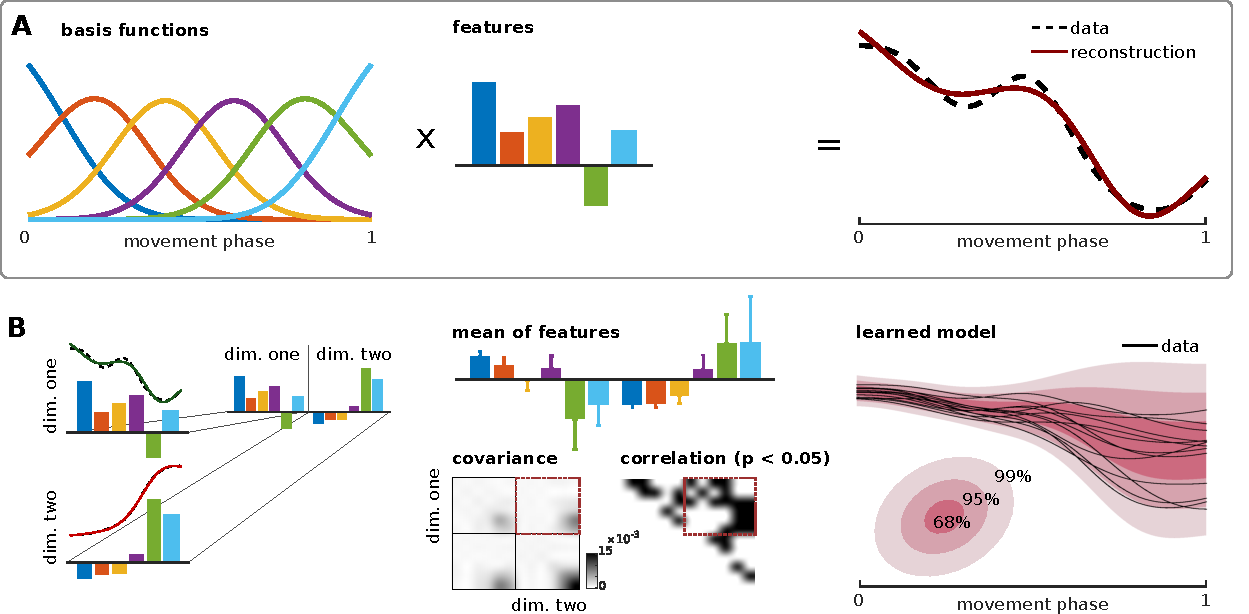
\includegraphics[width=1\textwidth]{Elmar/picsClean/AProbModelofMotionApproach1}
%\label{fig:subfig2}
 \caption{\textbf{Probabilistic model of trajectories, from a feature space (left column) to trajectories (right column):}  
 \textbf{A)} Generative model. 
 Equally spaced (radial) basis functions are amplitude scaled by a feature vector to approximate a one-dimensional trajectory. 
 A movement phase substitutes time to model trajectories of different lengths. 
 In the inverse direction, feature vectors are computed given the input trajectories using, e.g., standard linear regression techniques or 
 iterative variational approaches like expectation-maximization. 
 \textbf{B)} Learning the correlations between multi-dimensional input trajectories. 
 Feature vectors computed from multiple input trajectories are concatenated 
 and the mean and the covariance are computed from multiple trials (or subjects). 
 The learned correlation in the center panel is the key features for computing predictions from 
 partial observations. The distribution over trajectories is shown in the right panel. 
}
\label{fig:model}
\end{figure}

The main feature of the model is that it captures the correlations between 
individual input dimensions. The model builds on a linear function approximator 
using radial basis functions with fixed means and variances. 
The amplitudes are scaled by learnable features. Now both, the basis functions and the features,  
form a linear generative model of a trajectory, i.e., $\vec \tau = \vec \Phi \, 
\vec w$ (with the trajectory $\vec \tau = [y_1, y_2, ..., y_t]$, time-varying observations $y_t$, basis functions 
in $\vec \Phi$ and feature weights $\vec w$). \FigureAbbr 
\ref{fig:model}A shows the encoding of a single trajectory using classical radial 
basis functions. Note that the model is linear in the feature space, however it 
can capture non-linear dependencies in the trajectory space (through non-linear basis functions). The model's complexity is controlled 
through the number of basis functions. For the reaching experiments 
ten Gaussian distributions per dimension were found to be sufficient, see Supplementary \FigureAbbr \ref{fig:subFigNumGaussians}.

The feature vector 
$\vec w$ can be learned in the most simple case through standard linear 
regression or in more sophisticated models through one of the many existing 
variational inference methods \cite{Rueckert2015}. 

A PTM encodes multiple input dimensions through a concatenated feature vector (a 
two-dimensional example is illustrated in \FigureAbbrP 
\ref{fig:model}B). This concatenated feature vector scales the contribution of an 
\textit{extended} basis function matrix. Thus, the only difference to standard 
radial basis functions is a clever arrangement of basis functions and feature 
vectors to represent multiple input dimensions in one model. 
 
To model a distribution over trajectories the mean and the covariance over multiple trials are computed from the 
inferred feature vectors (e.g., through linear regression). An example is shown 
in the center panel in \FigureAbbr \ref{fig:model}B. The mean and 
the covariance encode a distribution over trajectories in the feature space and 
through the relationship $\vec \tau = \vec \Phi \, \vec w$, the distribution can 
be mapped (back) to the time domain. It is worth mentioning that a PTM can 
represent trajectories of varying lengths by substituting time by a movement 
phase. The last panel in \FigureAbbr \ref{fig:model}B shows an 
illustrative example of a trajectory distribution and the corresponding input 
trajectories using a movement phase.    

%Conclusion  
To conclude, the advantage of the presented time-series model is that it can be formulated as a 
generative probabilistic model for which many learning algorithms and similarity 
measures exist. The model can encode the signal variation and can be used to 
compute operations like predictions, model comparisons or trial likelihoods. 
These operations are explored in the present study on postural control with supportive 
contacts. 
%Implication the model can be used on an time series data and captures the correlation. Examples are EMG recordings, EEG channel encoding, temperature or force profiles, etc.   


\subsection{Supportive contacts predict goal-directed movements}

The learned and represented correlation of multiple limb trajectories can be 
exploited in computing predictions. This feature is used here to investigate if 
left wrist trajectories can predict the right wrist 
reaching trajectories. To separate the contributions of the trunk and the left 
arm, we transformed the wrist marker trajectories to a \textit{shoulder frame}. 
For that the wrist positions in the subject's coordinate frame were additionally 
corrected by the time-varying shoulder marker positions. 

\begin{figure}[t]
\centering
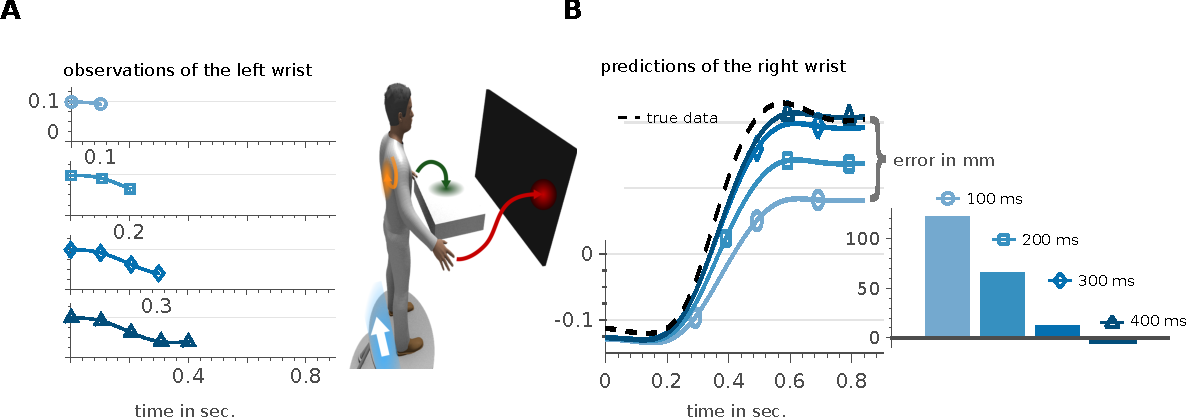
\includegraphics[width=\textwidth]{Elmar/picsClean/Fig3Predictions}
%\label{fig:subfig2}
 \caption{\textbf{Supportive contacts predict goal-directed movements:} 
 \textbf{A)} Partial observations of the left wrist predict right wrist future states in \textbf{B}. 
 For increasing observation horizons of the y-coordinate of the left wrist, 
 the predicted right wrist trajectories converge to the true trajectory (illustrated as dashed line in \textbf{B}). 
 The final Euclidean error (to the true reached target on the screen) of less than $2$ cm after $300$ ms is $40$ times smaller than the distance between the two outer targets (that is $80$ cm). 
}
\label{fig:OpsPrediction}
\end{figure}

For increasing observation horizons up to $400$ ms, exemplary predictions of the 
y-coordinate of the arm trajectories are shown in \FigureAbbr 
\ref{fig:OpsPrediction}. For these examples the target prediction error was 
below $5$ cm when observing only the first $300$ ms of the left wrist motion. 
Note that the distance between the two exterior targets on the screen was $80$ 
cm which defines the maximum error.  Averaged over all subjects, the prediction 
error was $12.3 \, \pm \, 9.8$ cm for an observation horizon of $300$ ms. When 
observing the complete trial the error was $6.4 \, \pm \, 5.5$ cm. Per subject errors are shown in \FigureAbbr 
\ref{fig:subFigPerdErrorAllSubjects}. Note that to obtain these results 
we used $18$ trials for training (trials $170-320$) and $18$ trials for testing (trials $321-400$). %six per target

\begin{figure}[t]
\centering
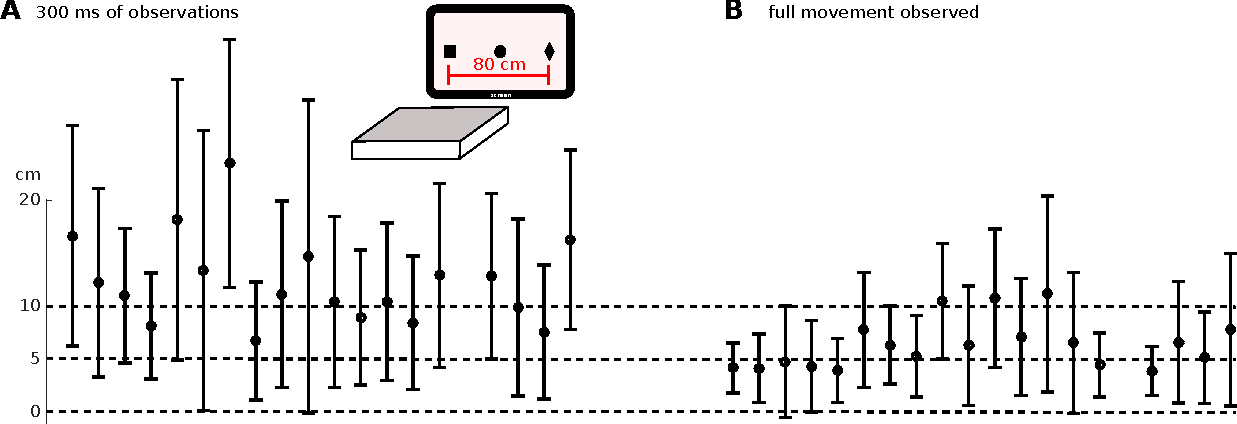
\includegraphics[width=\textwidth]{Elmar/picsClean/SubFigPredError9DoF}
%\label{fig:subfig2}
 \caption{\textbf{Target prediction error over all subjects:} 
 \textbf{A)} Averaged prediction error for $19$ subjects when observing $300$ ms of the left wrist marker trajectories in perturbed trials. 
 \textbf{B)} The prediction error when observing the whole left wrist motion. Illustrated are the mean and the 
 standard deviation over $18$ test trials (six per target). One subject of $20$ was excluded as less than six trials per target were recorded. 
 Note that the maximum error or the distance between the two outer targets in the screen is $80$ cm.
 }
\label{fig:subFigPerdErrorAllSubjects}
\end{figure}

%Conclusion: left wrist can predict the right wrist 
In summary, the PTM was used to train models of trajectory distributions that 
could predict the goal-directed reaching motions from observing solely the 
supportive left wrist movements. Accurate predictions at an early execution 
phase (i.e., the first $300$ ms), where the effect of visual feedback is 
negligible, indicate that supportive contacts are at least partially 
pre-processed. 

%Implication: Supportive contacts predict goal-directed movements

\subsection{Trunk adaptation precedes arm adaptation}

\begin{figure}[t]
\centering
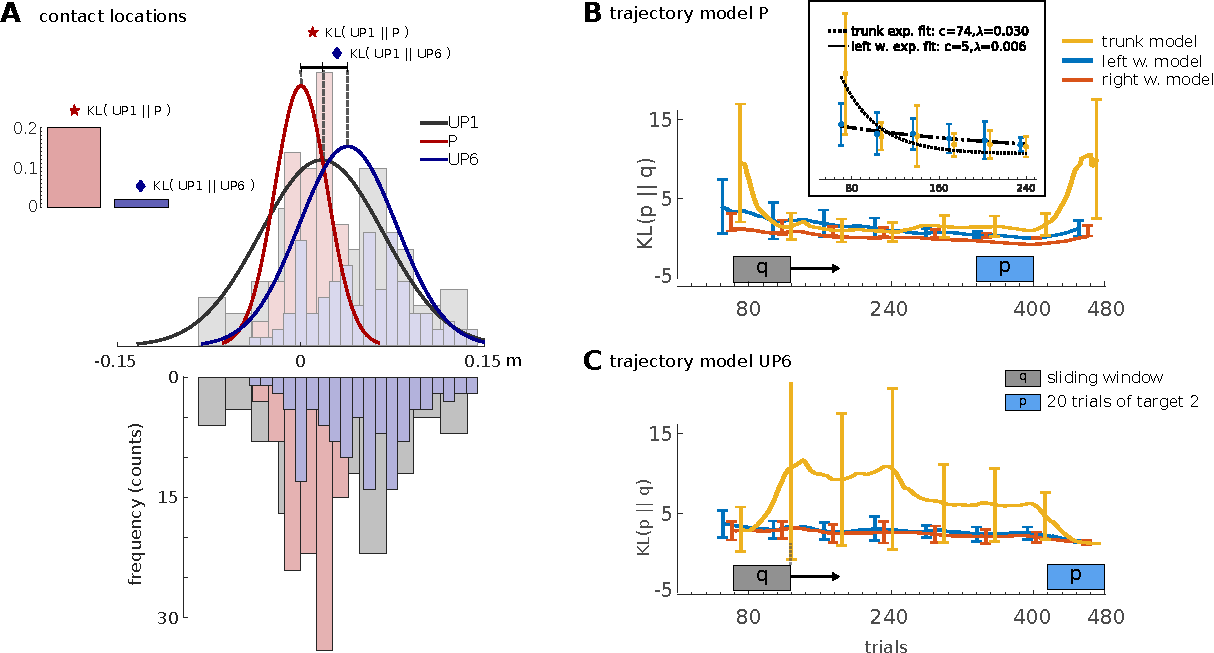
\includegraphics[width=\textwidth]{Elmar/picsClean/Fig4ModelComparison}
%\label{fig:subfig2}
 \caption{\textbf{Trunk adaptation precedes arm adaptation:} 
 \textbf{A)} The adaptation process of the contact location is illustrated by computing the KL-divergence between the first unperturbed session (UP1), the perturbed trials (P), 
 and the last unperturbed session (UP6). The underlying data is shown as histogram with the Gaussian model fits as overlay.
 \textbf{B-C)} For a detailed temporal analysis, the KL-divergence between a set of training trials (a sliding window of 20 trajectories) and 
 a set of test trials (\textbf{B}: last 20 trials in P, \textbf{C}: last 20 trials in UP6) is investigated. 
 An exponential model fit is presented in the inset in \textbf{B}.  
}
\label{fig:OpsModelComparison}
\end{figure}

To investigate adaptation of the supportive contacts we fitted Gaussian 
distributions to the contact locations recorded in the three phases of learning 
--- the unperturbed training phase, the phase of perturbed trials and the final washout phase. 
Histograms over the contact locations in the shoulder frame are shown in \FigureAbbr \ref{fig:OpsModelComparison}A, 
where \textit{UP1} denotes the initial training phase, \textit{P} the perturbed trials and 
\textit{UP6} the sixth session that was the washout phase. During the perturbed trials of the experiment, 
we found a shift of contacts to the right, or in other words, the left hand is moving closer to the 
center of the table in \FigureAbbr \ref{fig:subFigContactLocationsAllSubjects}A 
(Note that the particular values in meters differ in \FigureAbbrP 
\ref{fig:subFigContactLocationsAllSubjects}A and in \FigureAbbrP 
\ref{fig:OpsModelComparison}A. In the later the contacts are plotted in the 
shoulder frame).  

To compare the similarities between the fitted Gaussian distributions for the three phases of 
learning, we used a Kullback-Leibler divergence (KL) distance measure. 
In line with the observation of the shift of contacts, we 
found strong similarities between the unperturbed phases, i.e., KL(UP1$||$UP6) = 
$0.019$. In contrast for the transition to the perturbed trials we computed 
a distance of KL(UP1$||$P) = $0.20$. For the transition to the washout phase, 
we found KL(P$||$UP6) = $0.126$. 
%Note that for these comparisons the last six center targets in each phase of all subjects were used. 


A more detailed investigation was conducted by analyzing trajectory  
similarities using the PTM. As reference model, trajectories of the last $20$ 
trials in P or UP6 were used. We compared the reference model to a trajectory 
model trained from $20$ trials in a moving window. The moving window traverses from trial 
$10$ to trial $460$ which is denoted by the shaded boxes in \FigureAbbrP 
\ref{fig:OpsModelComparison}B and C. 
Individual models were trained for the left wrist, the right wrist and the 
trunk. We found that the trunk model converged about five times faster than the 
left wrist model. For that we used one-term exponential models of the form 
$y\,=\,c\,\exp(\lambda\,x)$, where for the trunk $\lambda_t=0.03$ and for the left wrist $\lambda_l=0.006$. 
This result is highlighted in the inlay in \FigureAbbr \ref{fig:OpsModelComparison}B.
% 
% with $c=74$ and $\lambda=0.03$ for the trunk 
% and $c=5$ and $\lambda=0.006$ for the left wrist. 
% 
% where for the trunk  
% % $c=74$, $\lambda=0.03$ vs. $c=5$, $\lambda=0.006$ for the left wrist where 
% % $0.03/0.006=5$)
% For the trunk the model parameters were $a=74$ and $b=0.03$ compared to . 
% (i.e., exponential fit of the trunk: 
% $c=74$, $\lambda=0.03$ vs. $c=5$, $\lambda=0.006$ for the left wrist where 
% $0.03/0.006=5$), see right column in \FigureAbbr \ref{fig:OpsModelComparison}B. 

We found that the trunk adapts faster than the supportive contact motion. This 
finding can be explained by the importance of correct trunk motions to prevent 
falling as observed in related work \cite{bouisset1981sequence, stapley1999does}. When comparing the prediction accuracy however, we made an interesting 
observation. During early phases of the motor execution the left wrist results 
in more accurate predictions. However, when observing the complete motion, the 
trunk was more informative for predicting the right arm movements, see 
Supplementary \FigureAbbr \ref{fig:SubFigPredErrorTrunkvsLW}. This result 
suggests that the supportive motion has a stronger effect on the task 
performance during early phases compared to the massive trunk. 

%Conclusion: Trunk adaption is more important for the task than wrist movement modifications
%Implication: Evidence for learning on multiple time scales


%DISCUSSION
\section{Discussion}

%controversy: static contacts are known to aid postural control, however it is unknown if they are planned or reactive???
It is known that supportive contacts aid postural control in humans 
\cite{balasubramaniam2002dynamics}. Contacts increase the subjects' belief about 
their poses in board balancing tasks \cite{slijper2000effects}, in tasks without 
visual cues \cite{johannsen2007effects}, and have an effect on learning 
balancing strategies during task adaptation \cite{babivc2014effects}. While 
these studies demonstrated the importance of contacts for human motor control, 
the contacts where \textit{static} and pre-defined based on the experimental 
setting. In this study, we investigated the effect of the \textit{active choice} 
of supportive contacts on motor control. Under natural conditions subjects were 
able to choose supportive contact locations to aid target reaching. Utilizing a 
developed probabilistic trajectory model (PTM), we found that the supportive motions 
leading to contacts could predict goal-directed reaching movements and 
learning proceeds on multiple time scales. These findings have important 
implications on medical care in diseases related to central nervous system 
disorders (such as dementia, Alzheimer's, Parkinson's disease or stroke), 
computational neuroscience and robotics. 

\subsection{A pre-test for central nervous system disorders affecting postural control} 

Many central nervous system disorders affect not only cognitive abilities 
related to memory consolidation but also postural control.  For example, an 
underdevelopment of postural control is a well known symptom in 
autism\cite{schmitz2003motor, minshew2004underdevelopment}. Early detection of 
these diseases is of utter importance for medical care. However, most pre-tests 
focus on cognitive functions that are influenced by many factors such as stress, 
sleep deprivation and age. Classical tests targeting motor coordination 
abilities are unnatural like for example the grooved pegboard 
test\cite{klove1963clinical}, where the goal is to fit pegs of various shapes 
into punched holes. The presented experimental setting has the 
potential to become an alternative pre-test that investigates postural control 
and motor learning under natural conditions. Deficits in motor control can be 
quantified in terms of the model prediction performance as shown in \FigureAbbr 
\ref{fig:OpsPrediction}. In the tested subjects, the average prediction error of the 
goal-directed target reaching motion was $6.4 \, \pm \, 5.5 \textrm{(SD)}$ cm out of a total range of 
$80$ cm. Note that for these predictions the model input was solely the x,y,z coordinate of 
the supportive motion, see \FigureAbbr \ref{fig:subFigPerdErrorAllSubjects}B. 
While the predictions were accurate for the tested healthy subjects, we speculate that 
participants with motor dysfunctions would show inferior prediction performance scores. 

However, a limitation of the presented experimental setting is its simplicity. 
In our experiments the participants reached for a static target at one out of three possible locations  
on a horizontal line. Synchronization of movement onsets within $3-5$ trials (see \FigureAbbr \ref{fig:subFigContactLocationsAllSubjects}C-D) 
indicates that the task might be too simple to show significant effects in subjects 
with central nervous system disorders. More complex tasks could consider for example moving 
targets at arbitrary locations on the screen. 

\subsection{Evidence for learning on multiple time scales}

For many tasks motor memory consolidation proceeds on 
different time scales\cite{wolpert2000computational, 
smith2006interacting, diedrichsen2010coordination}. In particular, postural 
control is adapted on a faster rate in contrast to goal-directed movements. For 
example, Huys et al. showed that postural sway precedes eye and head movements 
($3:2$ or also $3:1$) in subjects learning to juggle\cite{huys2004timescales}. 
In line with this finding, we found that trunk adaptation to maintain balance 
precedes the learning of optimal (here task correlated) supportive contact 
motions. Concretely, the learned trunk model converged about $5$ times faster 
than the left wrist model, see \FigureAbbr \ref{fig:OpsModelComparison}B. This result is 
another indicator for a hierarchical organization of motor control with the 
difference that we analyzed adaptation on a trajectory level in contrast to 
single time step models \cite{kuo1995optimal, wolpert2000computational, 
diedrichsen2010coordination}. The developed PTM  may extend future computational 
models for optimal feedback control by combining sequential predictions of feed 
forward commands and the integration of perceptual feedback. 

A potential deficit of such an optimal feedback controller is that we analyzed 
adaptation on a kinematic level, where limb inertia has a delayed effect on the 
recorded marker trajectories. For example, while expressive motion vectors can 
be observed for the light weight arms, the massive trunk may have moved just for 
few millimeters which could result in inaccurate predictions. This hypothesis is 
confirmed by our results, where at early movement phases (up to $300$ ms) the 
left wrist leads to more accurate predictions than the trunk, see Supplementary 
\FigureAbbr \ref{fig:SubFigPredErrorTrunkvsLW}. For observations of the complete 
trial however, the trunk motion is more informative. To avert the effect of limb 
inertia the PTM could be trained from Electromyography (EMG) patterns. Such 
models could be used to predict motor commands on a muscle level and could help to 
better understand the underlying motor control mechanisms. 

\subsection{A robot controller that actively seeks for contacts}

In this research we studied whole-body coordination mechanisms of arm reaching 
and postural control with additional hand contact. We investigated how humans 
perform reaching movements with the right arm in postural challenged conditions. 
Postural balance was maintained by establishing a supportive hand contact with 
the other arm. In effect, both arms had to perform reaching movements where one 
arm reaches for a distant target and the other arm reaches for a supportive hand 
contact. We found that humans preferred distinct contact locations for each of 
the three targets that were displayed. Such a context dependent controller could 
advance current abilities of humanoid robots as it was envisioned in the 
European project CoDyCo\cite{codyco}. In particular, our results suggest that 
different supportive contact strategies should be initiated based on future intentions. 
This has not been done so far as research on anticipatory controller 
 focused largely on balancing\cite{sugihara2002whole, rueckert2014robust, tassa2012synthesis} or 
 on compensating for external forces\cite{atkeson2007multiple, hyon2007full, ruckert2011study, toussaint2014dual}. 
%Work on contacts focused mainly on following force profiles for manipulation and 
% left postural control relatively unexplored. 

In our experiments the modulating factors (the context) were the distance to the 
target,  its location on the screen and the postural perturbation. The distance 
was chosen such that subjects \textit{always} made a contact to avoid falling 
when reaching. We only investigated the effect of the contact location and used 
pre-defined translateral support base perturbations. The perturbations had no 
effect on the results. In unperturbed and perturbed conditions the subjects 
chose target dependent contact locations, see \FigureAbbr 
\ref{fig:subFigContactLocationsAllSubjects}B. Future research may explore the 
effect of distance to complement a robot controller that autonomously decides in 
which situations to make supportive contacts. 


\section{Methods}%\label{sec:methods}

\subsection{Participants}

Twenty right-handed male subjects ($\textrm{age:} \, 20.8 \, \pm  \, 1.8 \,
\textrm{(SD)}$) participated in the reaching experiments. None reported any neurological or musculoskeletal
disorders (self-reported). Prior to their participation, the subjects were
informed about the course of the study and were required to sign an informed
consent approved by the National Medical Ethics Committee Slovenia (NO. 112/06/13).

\subsection{Apparatus}

Participants stood on a force plate (9281CA, Kistler Instrumente AG, Winterthur,
Switzerland) mounted on top of a Stewart platform \cite{stewart1965platform}.
The force plate was used to measure the six components of the ground reaction
forces and torques to determine the center-of-pressure (CoP). The CoP was only used 
to pre-compute tentative movement onsets (based on two percent peak velocity and CoP criteria).
These pre-computed movement onsets of the left and the right wrist were manually corrected through visual inspection ($480\,\times\,20$ trials). 
% In addition, fluctuations of force component in the superior direction were used
% to improve the movement onset computation based on wrist velocities (see
% Supplementary Fig. X2). 

A second force plate of the same type was mounted anteromedial to the subject's hip
position. This force plate was used like a table providing additional support 
during reaching. The contact locations shown in \FigureAbbr \ref{fig:subFigContactLocationsAllSubjects} were
defined as the left wrist position at the peak supportive contact force. In front to the 
contact force plate we mounted a screen. Both, the force plate and the screen
were adjusted in height based on the subject's trunk height ($56.5 \, \pm \, 2.4$ cm).
%NOTE to JAN: the third marker at the approx. CoM was not used in my code so far

The Stewart platform was used to apply translational perturbations in the 
mediolateral direction. Specifically, the displacement of the platform was 
proportional to the sum of the anteroposterior components of the left and right 
hand displacements. The maximal displacement of the Stewart platform was $20$ cm 
and corresponded to the situation when the subject's left hand was at the far 
edge of the table and the finger on the right hand touched the screen, see 
Supplementary \FigureAbbr \ref{fig:SubFigStewartPert}.

A motion capture system (NDI 3D Investigator) was used to track the participants 
wrists and trunk movements. Three motion tracking markers were attached two each wrist to 
compensate for occlusions during the reaching motions. At least one marker 
needed to be visible and for more than one visible marker the position was 
computed through averaging. Two markers were attached to the back at the 
scapulae to transform wrist trajectories to shoulder frames and to estimate the 
trunk motions (i.e., the center location of the two shoulder markers). 
Additional markers were placed at the screen, at a wearable thimble to estimate 
the right index fingertip position and at the force plate mounted on top of the 
Stewart platform.

\subsection{Coordinate frames}

If not stated different, the results are defined in the subject's coordinate
frame. To compensate for the translational perturbations of the Stewart platform
a marker was attached to the support force plate. The subjects coordinate frame
was defined as the force plate marker position minus the initial left wrist
location (to correct for small deviations of the subject's feet placement
throughout the experiment). 

Wrist trajectories (see \FigureAbbrP \ref{fig:OpsPrediction}) were computed in the shoulder frames to isolate
trunk and arm adaptations. In particular, the wrist positions in the subject's
coordinate frame were additionally corrected by the time-varying shoulder marker positions.  

\subsection{Procedure}

Participants had to perform $480$ trials of reaching in blocks of $80$ trials.
After each block the subjects had a five minutes break. Only the first and the
last $80$ trials were unperturbed (see \FigureAbbrP 
\ref{fig:subFigContactLocationsAllSubjects}b). To investigate
negative after effects, the perturbation was deactivated for $30$ randomly selected reachings  
during trials $240$ to $400$. The participants were not informed about these
catch trials. 
%5     9    14    19    22    26    32    36    41    47    51    57    64    69     73    79

Prior to each trial, subjects were required to stand upright moving as little as
possible. A bar on the screen indicated anteroposterior fluctuations of the CoP
in real time with respect to the initial CoP value. This initial CoP was measured at the beginning of
the experiment. If the mean of the deviations averaged over $500$ ms was less
than $1$ cm the start of the trial was initiated. After one second the target
was presented at one out of three locations (target onset). After a random
period ($1-3$ sec) the target's color switched and the subjects were allowed to
move. Movements prior to that visual cue terminated the trial. The target was
reached if the distance between the fingertip and the target on the screen was
less than $1$ cm. 

Participants received a monetary reward after each trial based on the time
needed for reaching, i.e., $\textrm{EUR}\,=\,0.1 \, - \, 0.05 \, t\,$ where $t$ denotes the reaching time in seconds. 
The reaching time was defined as the difference between the target onset and the time until the target
was reached. On average the subjects received five cents per trial which corresponds to a reaching duration of one second, see Supplementary \FigureAbbr \ref{fig:SubFigRewards}. %On average our subjects earned $20X \, \pm \, xx$ EUR.
 If the target was missed, or if the target was not reached within
two seconds, no reward was given. 

\subsection{Data processing}

All measurements of the force plates and the motion capture system were recorded at a rate of $100$ Hz. Redundant marker settings on the
wrists and on the thimble were used to compensate for occlusions. For that three markers were used 
for both wrists and the thimble. If all markers were occluded the trial was excluded from the analysis. 
For two or three correctly observed markers we computed the average for each coordinate (x,y,z). 
All marker trajectories were low-pass filtered at $5$ Hz using $2$nd-order Butterworth filter.
% Fs = 100; %100Hz
%     Fc = 5; %Hz
%     order = 2;
%     [f, e] = butter(order, Fc*2/Fs, 'low');


\subsection{Statistical tests}

Statistical analyses were performed using SPSS 21 (SPSS Inc., Chicago, USA). For 
each subject, an average of left hand contact location in mediolateral direction 
was calculated for every combination of balance perturbation (unperturbed, 
perturbed and unperturbed catch trials) and target locations. The average values 
of the individual subjects were then used for statistical analysis. Effect of 
perturbation was investigated using one-way repeated measures ANOVA. Differences 
between perturbed and unperturbed sessions for each combination of independent 
variables were tested with post hoc t-tests with Bonferroni correction. The 
level of statistical significance was set to $0.05$.
    
\subsection{Computing predictions through conditioning}
%
Conditional probabilities and predictions are related concepts in statistical
modeling. A prediction problem can modeled as computing the conditional
probability denoted by 
\begin{equation}
p(B \, | \, A) = p(A,B) \, / \, p(A) ~~, \label{eq:cond_prob}
\end{equation}
where $A$ and
$B$ represent two random variables (RVs). In our experiment, the variable $A$
could encode the probability of a certain contact location on the table and the
target location is represented by the RV $B$. The joint distribution $p(A,B)$ is
the learned model and $p(A)$ is a prior over all possible contact locations.
Given a particular contact location $p(A=a)$, we can compute the most likely 
target the human tries to reach. Throughout the paper, we will use the shorthand
$p(a)$ to denote $p(A=a)$, which is the probability that the RV $A$ takes the
value $a$ to keep the notation uncluttered. 

A particular interesting class of distributions are Gaussian distributions 
\begin{equation}\label{eq:gaussian}
 N(\vec x \, | \, \vec \mu, \vec \Sigma) \coloneqq \frac{1}{{(2\pi)}^{n/2} \, \sqrt{\textrm{det} \vec \Sigma}} \, 
    \exp \left( -\frac{1}{2} (\vec x - \vec \mu)^T \, \vec \Sigma^{-1} \, (\vec x - \vec \mu) \right) ~~,
\end{equation}
 with the $n$-dimensional RV $\vec x \in \mathbb{R}^n$, the mean $\vec \mu$ and the variance $\vec \Sigma$. 
%, i.e. $\N(x | \mu, \Sigma)$ with the RV $x$, mean $\mu$ and variance $\Sigma$. 
In Gaussian distributions, conditional distributions can be computed in closed form. To see
this, we define a multivariate normal distribution by concatenating two RVs. The two RVs denote the contact locations and the targets, i.e., $\vec x = {a \choose b}$, $\vec \mu =
{\mu_a \choose \mu_b}$ and $\vec \Sigma = \left( \begin{smallmatrix}
\Sigma_{aa}&\Sigma_{ab}\\ \Sigma_{ba}&\Sigma{bb} \end{smallmatrix} \right)$. 
Using these definitions  
in \eqref{eq:gaussian} and after rearranging the terms, the
parameters $\mu_{b|a}$ and $\Sigma_{b|a}$ of the conditional distribution can be computed as 
\begin{eqnarray}\label{eq:general_cond_param}
  p(b \, | \, a) \;&=&\; \N(b \, | \, \mu_{b|a},\Sigma_{b|a}) ~~, \\
   & \text{with} & ~~~ \mu_{b|a}  =  \mu_b + \Sigma_{ba} {\Sigma_{bb}}^{-1} (a - \mu_a) ~~, \nonumber\\
  & \text{and} & ~~~ \Sigma_{b|a} = \Sigma_{bb} - \Sigma_{ba}{\Sigma_{bb}}^{-1}\Sigma_{ab}  ~~. \nonumber
\end{eqnarray}
Given multiple measurements of $a$ and $b$ we can compute the statistics $\vec \mu$ and
$\vec \Sigma$. For some during training unseen contact location $a^*$ we can now
predict the most likely target location (parametrized through $\mu_{b|a^*}$ and
$\Sigma_{b|a^*}$). In the following we will extend this powerful feature of computing predictions to time-series data or trajectories. 

\subsection{Phase modulated probabilistic models of trajectories}
%minimal description, details are given in Box 1
The same conditioning operation can be used for computing predictions in trajectories if the RVs 
encode feature vectors in function approximation, see \FigureAbbr \ref{fig:model} for a sketch. 
Let $\vec y_t = {a_t \choose b_t}$ denote a concatenated state at time $t$ representing the contact location and the target. 
Only for the sake of clarity we will again assume that the contact location and the target are 
scalars. As we will see later the results generalize to multi-dimensional states. 
In addition, we will assume for simplicity that each dimension in $\vec y_t$ is 
approximated through a $J$-dimensional feature vector $\vec w \in \mathbb{R}^{J \times 1}$ 
and basis function vectors $\vec \phi_t \in \mathbb{R}^{1 \times J}$, 
e.g.  $a_t = \vec \phi_t \, \vec w_a$ with $\vec \phi_t = \left[\phi_{t,1},\, ..., \, \phi_{t,J}\right]^T$. 
A large variety of possible basis functions can be used for time series approximation. A popular choice 
for rhythmic movements are Von-Mises basis functions, 
whereas Gaussian basis functions are widely used for point to point movements \cite{Rueckert2013, ijspeert2013dynamical} 
\begin{equation*}
 \phi_{t,i} = \frac{1}{\mathcal{Z}} \, \exp \left( -\frac{1}{2 h} \left(z(t) - c_i \right)^2 \right) ~~,
\end{equation*}
where $\mathcal{Z} = \sum_{l=1}^J \exp \left( -1\,/\,2 h \left(z(t) - c_l \right)^2 \right)$ denotes a normalization term.  
The function $z(t)$ implements a mapping from discrete time steps to a movement phase, i.e., $z: t \in [1,T] \mapsto [0,1]$. 
In this notation state sequences of different length can be modeled and are aligned through the movement phase. 
Note that in our reaching experiments $z(t)=0$ denotes the movement onset and $z(t)=1$ the event when the target was reached. 
The scalar $c_i \in [0,1]$ denotes the center of the $i$-th basis function and $h$ is the bandwidth 
parameter. 

In general, $D$-dimensional states can be approximated in $\vec y_t = \vec
\Phi_t \; \vec w$ using block diagonal matrices $\vec \Phi_t \in \mathbb{R}^{D
\times J D}$ and concatenated feature vectors $\vec w = \left[w_1^T,\, ...,\,
w_D^T\right]^T \in \mathbb{R}^{J D \times 1}$. For example, when modeling
contacts and targets,  $\vec w = \left[w_a^T, w_b^T\right]^T$ and a block
diagonal matrix of the form $\vec \Phi_t = \left( \begin{smallmatrix} \vec
\phi_t & \vec 0 \\ \vec 0 & \vec \phi_t \end{smallmatrix} \right)$ is used. 

Sequences of $T$ states, denoted by $\vec \tau = \vec y_{1:T}$, can be compactly represented by 
\begin{eqnarray}
    \vec \tau \;=\; \vec \Phi_{1:T} \, \vec w ~~~~ 
    \text{with} ~~~~ \vec \Phi_{1:T} = \left[\vec \Phi_1^T,\, ...,\, \vec \Phi_T^T\right]^T \in \mathbb{R}^{T D \times J D} ~~,  \label{eq:func_approx_general} 
\end{eqnarray}
where $\vec \Phi_{1:T}$ denotes an extended basis function matrix. 
Using the function approximation in \eqref{eq:func_approx_general} we can define the 
generative probabilistic model for trajectories 
\begin{equation*}
p(\vec \tau \, | \, \vec w) = \prod_{t=1}^T \N\left(\vec y_t \middle| \vec \Phi_{t} \, \vec w, \vec \Sigma_y \right)  \; = \; \N\left(\vec y_{1:T} \middle| \vec \Phi_{1:T} \, \vec w, \vec \Sigma_y \right) ~~,   
\end{equation*}
where $\vec \Sigma_y$ models zero mean independent and identically distributed (i.i.d.) Gaussian noise in $\vec y_t = \vec \Phi_t \; \vec w + \vec \epsilon_y$ 
with $\vec \epsilon_y \sim \N\left(\vec \epsilon_y \, | \, \vec 0, \vec \Sigma_y \right)$. 
%
In order to represent a distribution over trajectories $p(\vec \tau)$, 
we can apply the product rule shown in \eqref{eq:cond_prob} and compute the marginal. 
For Gaussian distributions, in particular for $p(\vec w) = \N\left(\vec w\middle| \vec \mu_w, \vec \Sigma_w \right)$, 
the marginal can be computed in closed form 
\begin{eqnarray}
  p(\vec \tau) &=&  \int p(\vec \tau \, | \, \vec w) p(\vec w) d\vec w \nonumber \\
    &=&  \int \N\left(\vec y_{1:T} \, | \,  \vec \Phi_{1:T} \, \vec w, \vec \Sigma_y\right)  \N\left(\vec w \, | \, \vec \mu_w, \vec \Sigma_w\right) d\vec w \nonumber \\
    &=& \N\left(\vec y_{1:T} \, | \, \vec \Phi_{1:T} \, \vec w,\; \vec \Phi_{1:T} \, 
      \vec \Sigma_w \, \vec \Phi_{1:T}^T + \vec \Sigma_y\right) ~~. \label{eq:feature_to_traj}
\end{eqnarray}
The mean $\vec \mu_w$ 
and the covariance matrix $\vec \Sigma_w$ can be learned from data by maximum likelihood using the Expectation Maximization (EM) algorithm \cite{Dempster1977}. 
A simpler solution that works well in practice is to compute first the most likely estimate of $\vec w^{[i]}$ for each trajectory $\vec \tau^{[i]}$ independently,  
where the index $i$ denotes the $i$-th demonstration.   
In particular, given the trajectory $\vec \tau^{[i]}$, the corresponding 
weight vector $\vec w^{[i]}$ can be estimated by a straight forward least squares estimate
\begin{equation}
 \vec w^{[i]} = \left(\vec \Phi_{1:T}^T \, \vec \Phi_{1:T} + \lambda \, \vec I\right)^{-1} \, \vec \Phi_{1:T}^T \; \vec \tau^{[i]} ~~. \label{eq:lin_reg_traj}
\end{equation}
Subsequently, the mean and the covariance of $p(\vec w)$ can be estimated 
by the sample mean and sample covariance of the $\vec w^{[i]}\,$ vectors. 

\subsection{Computing predictions in trajectories}
%partial spatio-temporal observations encoded in o, \Phi_o and \Sigma_o
Let us assume that we have observed a sequence of states $\vec y_{t_1}$ to $\vec y_{t_M}$ at $m=1,2, ..., M$ different time points, 
which do not need to be sampled at uniform intervals. In addition, not all of the dimensions in the vector 
$\vec y_{t_m}$ might be observed (e.g. due to occlusions, where irrelevant dimensions are assumed to be set to some real number). 
We introduce the homogeneous covariance matrix $\boldsymbol{\Sigma}_{\vec o}$ to control the importance of the observations, 
where small diagonal variances denote important dimensions and large scalars irrelevant dimensions. 
For example, we would use $\boldsymbol{\Sigma}_{\vec o} = \left( \begin{smallmatrix} 1e-5&0\\ 0&1e5 \end{smallmatrix} \right)$ 
if only the first out of two dimensions is observed (as in the example with contact locations and targets). 
Let us further denote $\vec \Phi_{\vec o}$ as the concatenation of the basis function matrices for these time points 
and $\vec o$ as concatenation of the $\vec y_{t_m}$ vectors. 
Given these observations, we can obtain a conditioned distribution $p(\vec w| \vec o)$ over the weight vectors 
%conditioning result
\begin{eqnarray*}
    p(\vec w_o \, | \, \vec o) \;& \propto &\; \N(\vec o \, | \, \vec \Phi_{\vec o} \, \vec w_o, \boldsymbol{\Sigma}_{\vec o}) \, p(\vec w) ~~ \\
     \;& \coloneqq &\; \N(\vec w_o \, | \, \boldsymbol{\mu}_{\vec w| \vec o}, \boldsymbol{\Sigma}_{\vec w|\vec o}) ~~, \\
    & \text{with} & ~~~ \boldsymbol{\mu}_{\vec w| \vec o}  =  \boldsymbol{\mu}_{\vec w} + 
      \boldsymbol{\Sigma}_{\vec w}\boldsymbol{\Phi}_{\vec o}^T\left(\boldsymbol{\Sigma}_o + 
      \boldsymbol{\Phi}_{\vec o}\boldsymbol{\Sigma}_{\vec w}\boldsymbol{\Phi}_{\vec o}^T\right)^{-1}\left(\vec o -\boldsymbol{\Phi}_{o}\boldsymbol{\mu}_{\vec w}\right) ~~,  \\
    & \text{and} & ~~~ \boldsymbol{\Sigma}_{\vec w|\vec o} =  \boldsymbol{\Sigma}_{\vec w}-
      \boldsymbol{\Sigma}_{\vec w}\boldsymbol{\Phi}_{\vec o}^T\left(\boldsymbol{\Sigma}_o 
      +\boldsymbol{\Phi}_{\vec o}\boldsymbol{\Sigma}_{\vec w}\boldsymbol{\Phi}_{\vec o}^T\right)^{-1}\boldsymbol{\Phi}_{\vec o} \boldsymbol{\Sigma}_{\vec w} ~~, 
\end{eqnarray*}
which recovers the conditioning result in \eqref{eq:general_cond_param} in the feature space. 
%prediction result

To predict the state sequence $\vec{\tilde{y}_{1:T}}$, the 
conditional distribution is projected back into the trajectory space using \eqref{eq:feature_to_traj}. 
The result is a distribution over trajectories %Our goal is to predict future states $\vec \tilde{y}_1:T$ given the observations $\vec o$. 
\begin{eqnarray}
  p(\vec \tilde{\tau}) = \N\left(\vec{\tilde{y}_{1:T}} \, \middle| \, \vec \Phi_{1:T} \, \boldsymbol{\mu}_{\vec w| \vec o} \, , \, \vec \Phi_{1:T} \, 
		  \boldsymbol{\Sigma}_{\vec w|\vec o} \, \vec \Phi_{1:T}^T + \vec \Sigma_y\right) ~~, \label{eq:cond_prob_traj}
\end{eqnarray}
where for $t_M < T$ in the observations $\vec o = [\vec y_{t_1}, \vec y_{t_2}, \dots, \vec y_{t_M}]$ future states can be predicted.

\subsection{Computing model comparisons in trajectories}

Using the proposed probabilistic trajectory model (PTM), two trajectory models can be compared through computing the Kullback-Leibler (KL) divergence. 
For Gaussian distributions as in \eqref{eq:feature_to_traj} the KL divergence can be computed in closed form 
\begin{eqnarray*}
 \textrm{KL}(\N_1 || \N_2) = \frac{1}{2} \, { \log \, \frac{ |\vec{\Sigma_2}| }{ |\vec{\Sigma_1}| } \, - n \, + \textrm{tr}({\vec{\Sigma_2}}^{-1} \vec{\Sigma_1}) 
 + (\vec{\mu_2} - \vec{\mu_1})^T \, {\vec{\Sigma_2}}^{-1} \,  (\vec{\mu_2} - \vec{\mu_1}) 
 \, } ~~,  
\end{eqnarray*}
where $\N_1$ denotes a Gaussian with the $n$-dimensional mean $\vec{\mu_1}$ and the covariance $\vec{\Sigma_1}$. The symbol $\textrm{tr}$ denotes the matrix trace. 

\subsection{Computing task likelihoods in trajectories}

Another important probabilistic operation is the computation of the task likelihood. 
This operation can be used to test which candidate model out of several best explains the data. 
Let $\N_p(\, . \, | \, \vec{\mu}, \, \vec{\Sigma})$ denote the model under test. 
Given a single trajectory sample $\vec \tau^*$ and its feature space representation $\vec w^*$ we can compute  
\begin{eqnarray*}
 \textrm{L}(\vec w^* | \N_p) &=& \log \, \N_p(\vec w^* \, | \, \vec{\mu}, \vec{\Sigma} ) \\ 
 &=& - \frac{1}{2} (\vec{\mu} - \vec w^*)^T \, {\vec{\Sigma}}^{-1} \,  (\vec{\mu} - \vec w^*) \, + \, \textrm{a constant} ~~,  
\end{eqnarray*}
which quantifies how likely $\vec \tau^* = \vec \Phi_{1:T} \, \vec w^*$  was generated by model $\N_p(\, . \, | \, \vec{\mu}, \, \vec{\Sigma})$. 


%\renewcommand{\thesection}{S\arabic{section}}  
%\renewcommand{\thetable}{S\arabic{table}}  
%\renewcommand{\thefigure}{S\arabic{figure}} 
%\renewcommand{\theequation}{S\arabic{equation}} 

\section{Supporting Information}

\begin{figure}
\centering
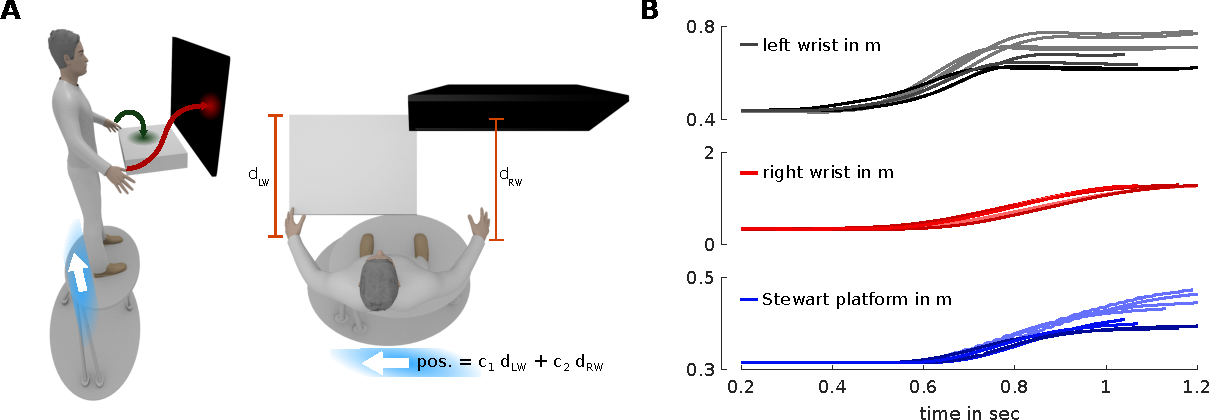
\includegraphics[width=\textwidth]{Elmar/picsSupp/SubFigStewartPert}
%\label{fig:subfig2}
 \caption{\textbf{Supplementary figure, Translateral perturbations:} 
 \textbf{A)} The Stewart platform was used to apply translational perturbations in the mediolateral direction. Specifically, the displacement of the platform was proportional to the sum of the anteroposterior components of the left and right hand displacements. This is denoted by $d_{\textrm{LW}}$ and $d_{\textrm{RW}}$ with the constants $c_1$ and $c_2$. The maximal displacement of the Stewart platform was $20$ cm and corresponded to the situation when the subject's left hand was at the far edge of the table and the finger on the right hand touched the screen. \textbf{B)} Sample trajectories of the left wrist, the right wrist and the displacement of the platform. 
 }
\label{fig:SubFigStewartPert}
\end{figure}


\begin{figure}
\centering
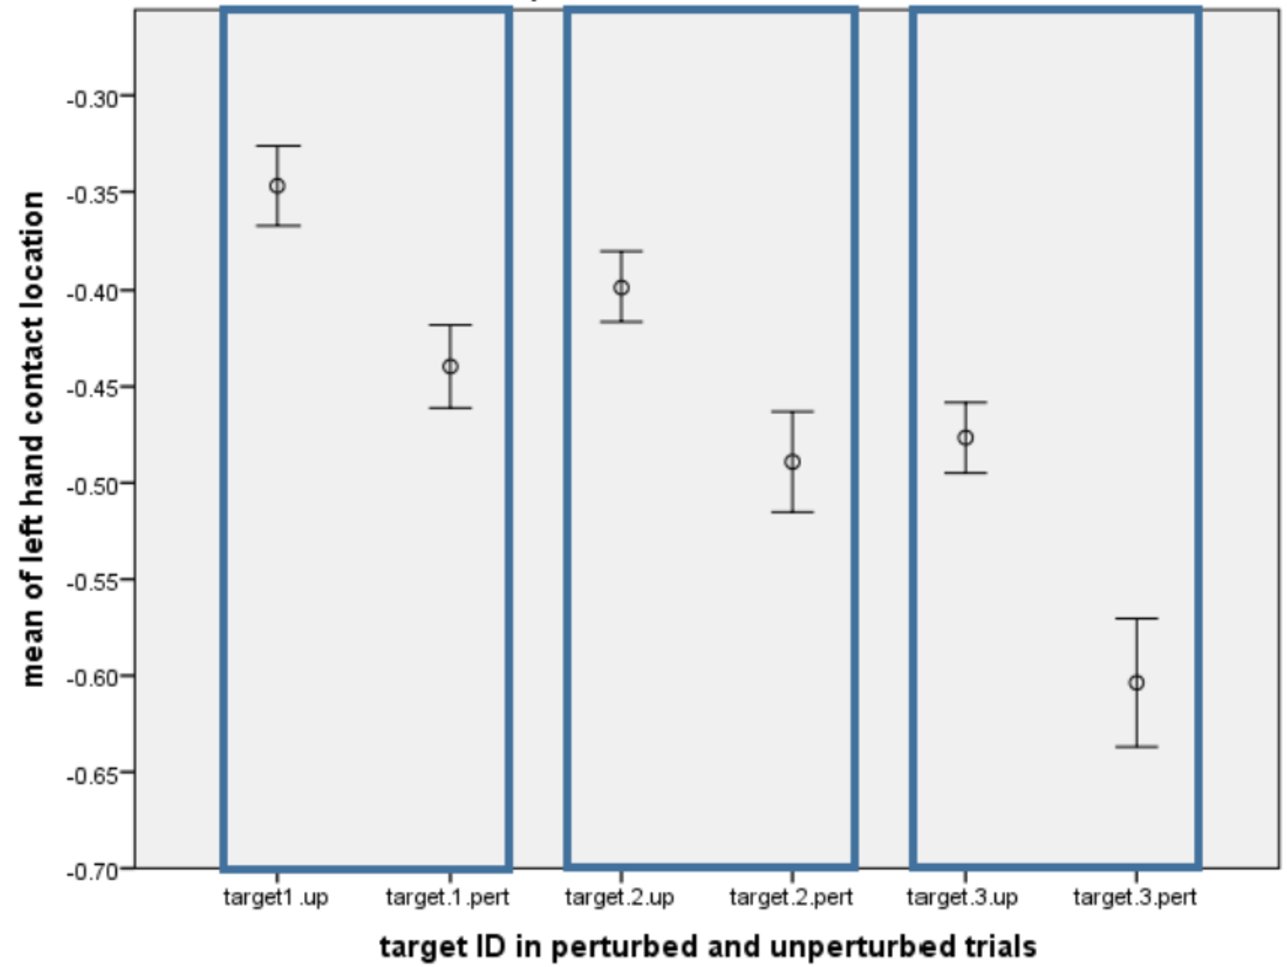
\includegraphics[width=.7\textwidth]{Elmar/picsSupp/SubFigANOVAContactsUPvsPNoTitle}
%\label{fig:subfig2}
 \caption{\textbf{Supplementary figure, Means of the contact locations:} 
 From left to right the means are shown for the three target locations, where we contrast in each panel the unperturbed and the perturbed session.  
 }
\label{fig:SubFigANOVAContacts}
\end{figure}



% \begin{figure}
% \centering
% 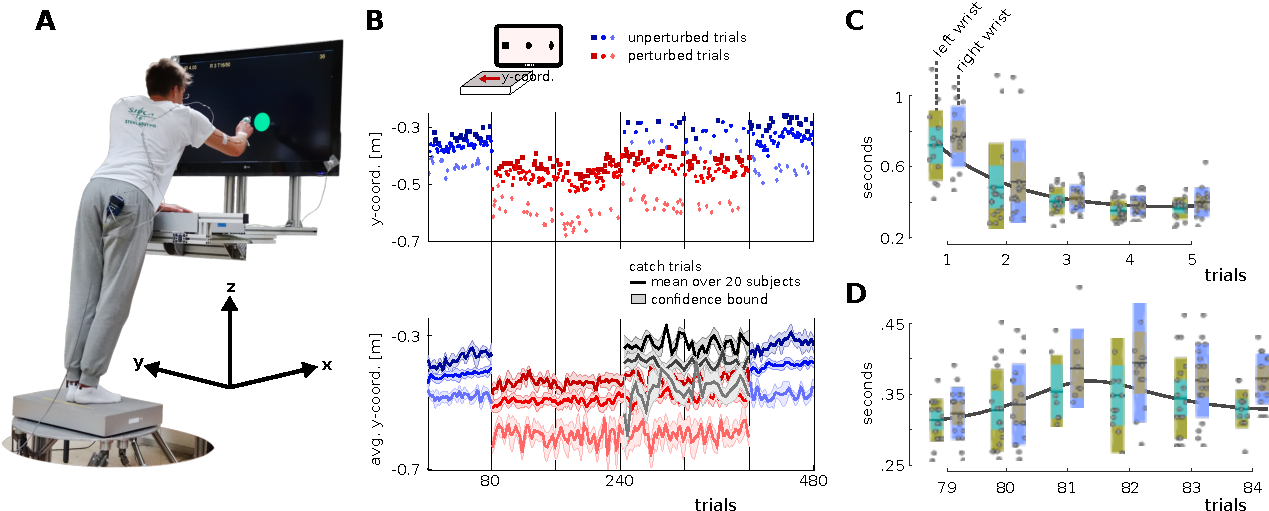
\includegraphics[width=\textwidth]{Elmar/picsClean/Fig1ExperimentContactsOnsets}
% %\label{fig:subfig2}
%  \caption{\textbf{Experiment and Adaptation:} (a) Experimental setting. 
%  (b) The top row shows contact locations for a single representative subject 
%  and the bottom row shows the mean and the confidence bound over all $20$ subjects. 
%  The first $80$ trials and the last $80$ trials ($400$ to $480$) are unperturbed sessions. 
%  Catch trials were initiated during trials $240$ to $400$. Note that during catch trials the contact 
%  location immediately switches back to the unperturbed behavior. This can be explained by the fact that the contact location 
%  is a result of both, the trunk motion (which shows strong negative after effects) and the left wrist motion (were we could not find these effects). 
%  Another finding is that contact locations are target correlated denoted by the three lines in (b). 
%  (c) Illustration of the movement onsets of the wrists for the first five trials (top row) and for the trials transitioning to the first perturbed session (bottom row). 
% }
% %\label{fig:subFigContactLocationsAllSubjects}
% \end{figure}


\begin{figure}
\centering
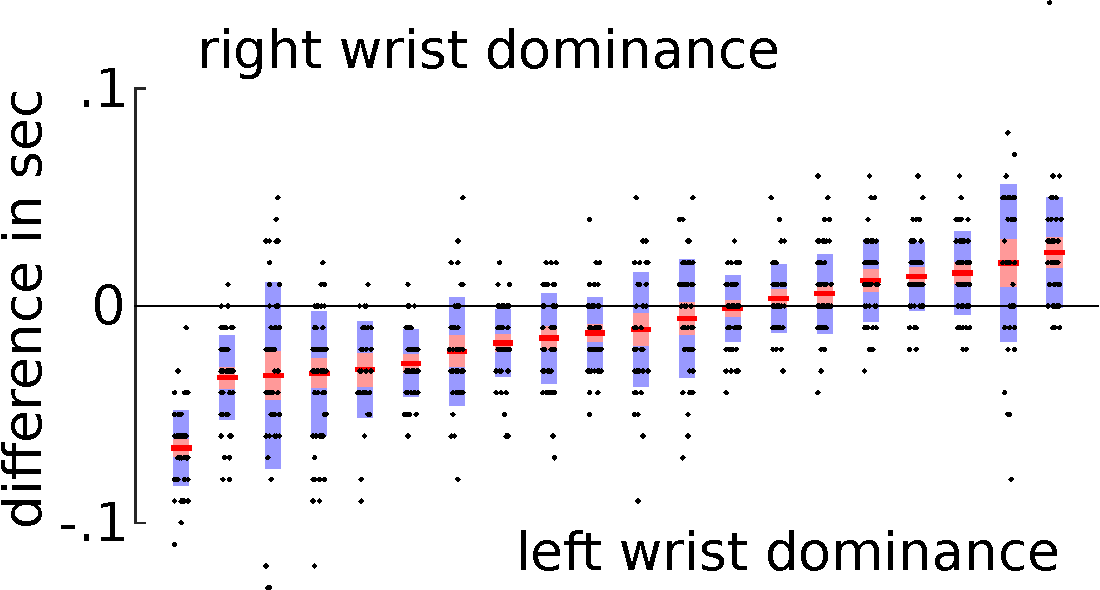
\includegraphics[width=.6\textwidth]{Elmar/picsSupp/SubFigWristPriorities}
%\label{fig:subfig2}
 \caption{\textbf{Supplementary figure, Dominance of the left wrist in 12 out of 20 subjects:} We show the difference of the movement onsets (left wrist minus right wrist). 
 The underlying data are representative trials of the $2$nd perturbed session ($170$ to $240$), where learning converged. The movement onsets were manually corrected through visual inspection. 
 }
\label{fig:subFigWristPriorities}
\end{figure}

% \begin{figure}
% \centering
% 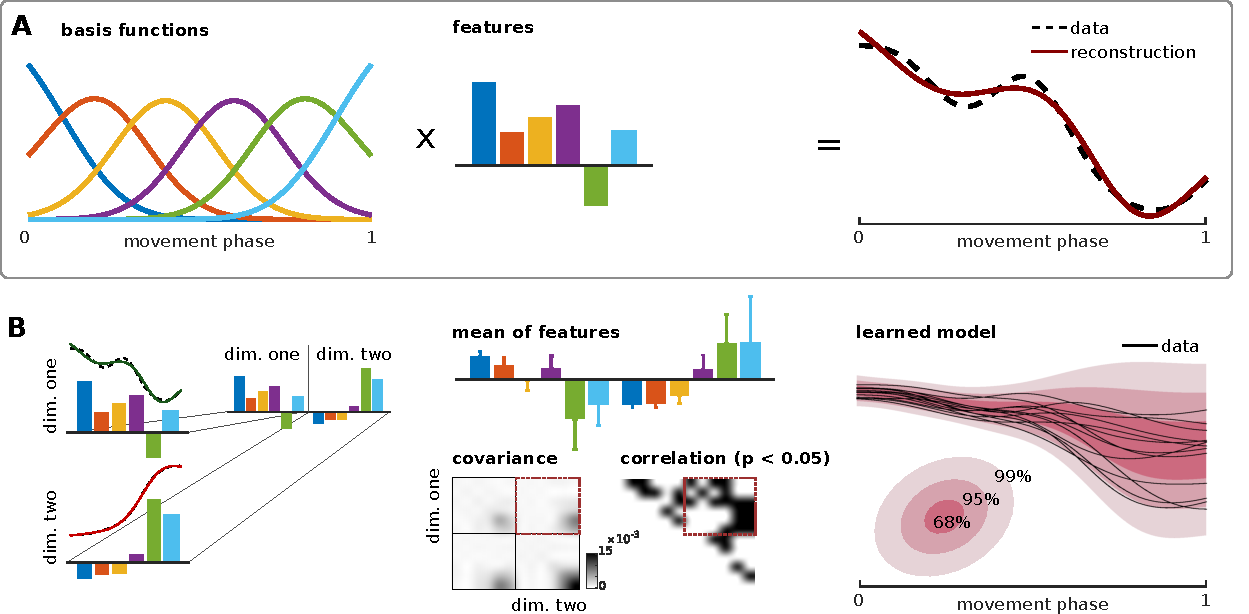
\includegraphics[width=1\textwidth]{Elmar/picsClean/AProbModelofMotionApproach1}
% %\label{fig:subfig2}
%  \caption{\textbf{Probabilistic model of trajectories, from a feature space (left column) to trajectories (right column):}  
%  (a) Generative model. 
%  Equally spaced (radial) basis functions are amplitude scaled by a feature vector to approximate a one-dimensional trajectory. 
%  A movement phase substitutes time to model trajectories of different lengths. 
%  In the inverse direction, feature vectors are computed given the input trajectories using, e.g., standard linear regression techniques or 
%  iterative variational approaches like expectation-maximization. 
%  (b) Learning the correlations between multi-dimensional input trajectories. 
%  Feature vectors computed from multiple input trajectories are concatenated 
%  and the mean and the covariance are computed from multiple trials (or subjects). 
%  The learned correlation is the key features for computing predictions from 
%  partial observations or different input dimensions than the predicted one (e.g., predicting the right wrist trajectory given the left wrist traj. in reaching). 
% }
% \label{fig:model}
% \end{figure}

\begin{figure}
\centering
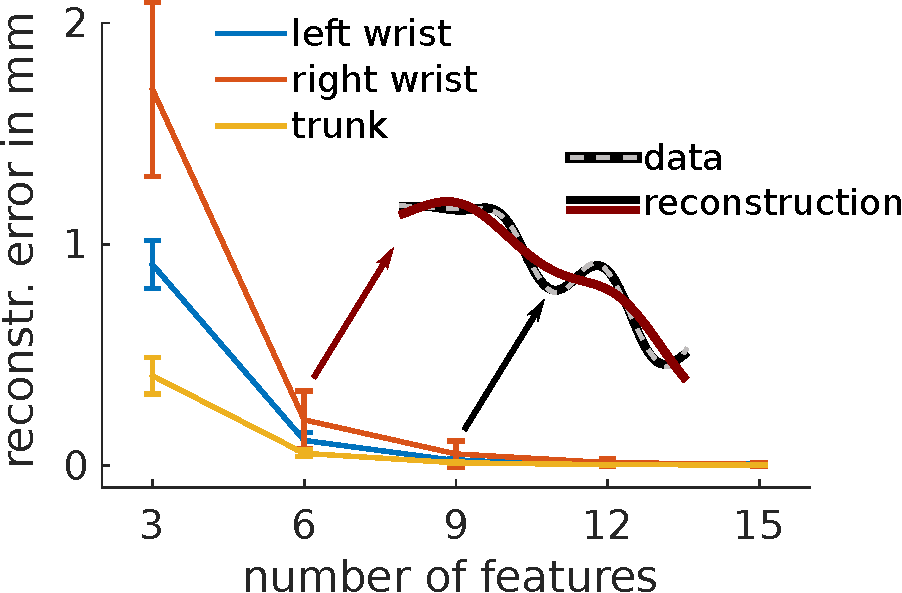
\includegraphics[width=.5\textwidth]{Elmar/picsSupp/NumGaussianFeatures}
%\label{fig:subfig2}
 \caption{\textbf{Supplementary figure. Model complexity (number of basis functions) determines the reconstruction error:}  
 With an increasing number of basis functions the reconstruction error (shown in millimeter) decreases. 
 The reconstruction error is defined as the Euclidean distance of the generated trajectory to its observed counterpart. 
 For the three limbs, left wrist, right wrist and trunk, the error converges to zero with more than nine basis functions. 
 Ten basis functions are used in the experiments in the manuscript. 
}
\label{fig:subFigNumGaussians}
\end{figure}

% \begin{figure}
% \centering
% 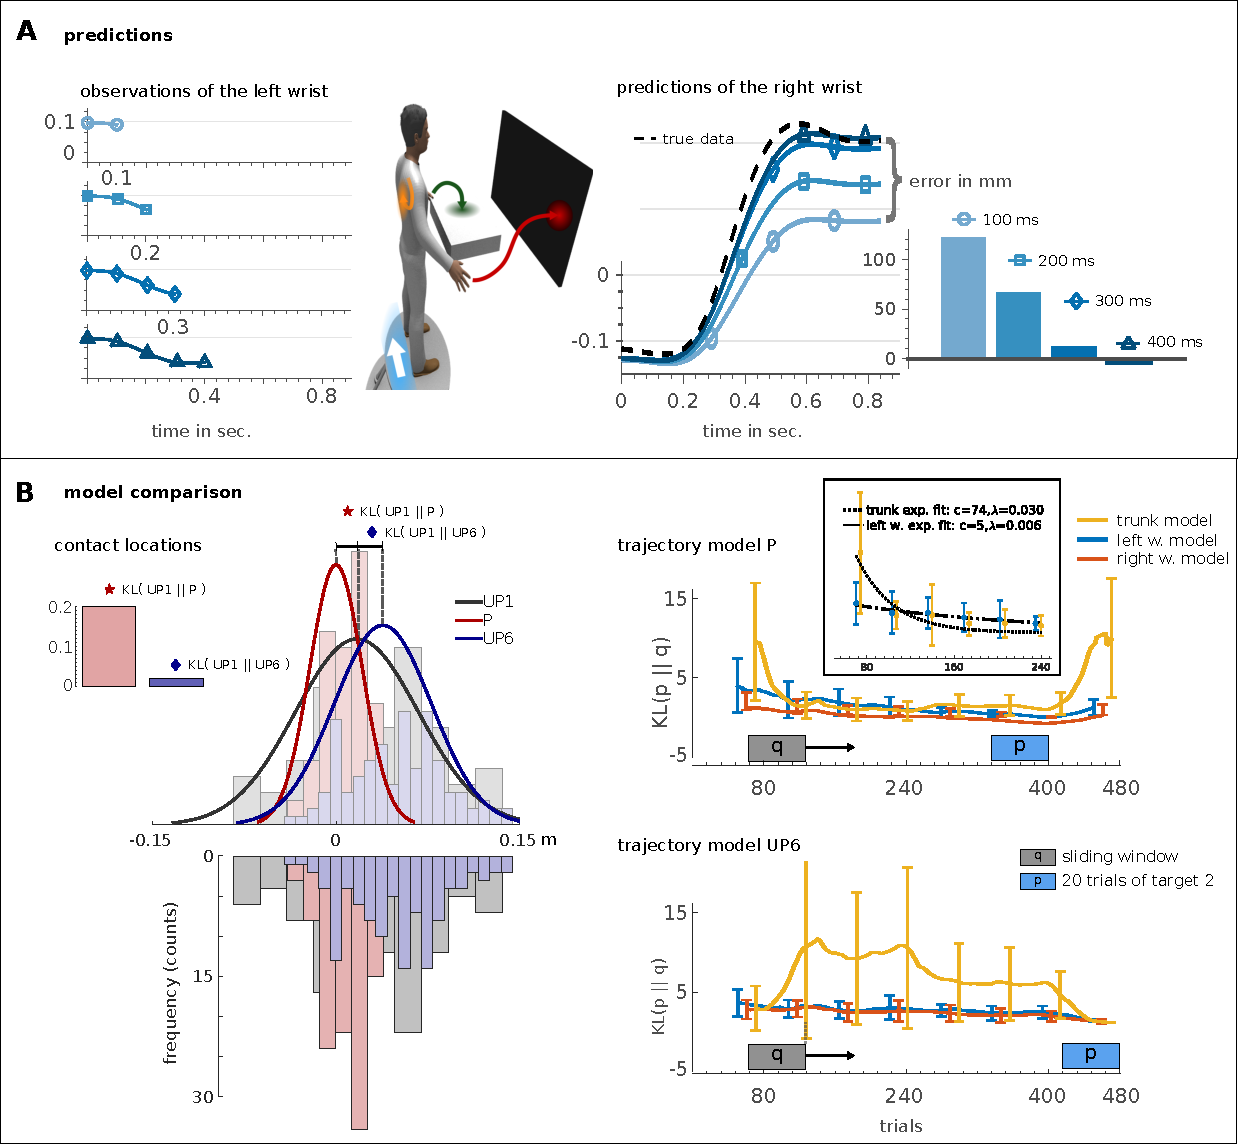
\includegraphics[width=\textwidth]{Elmar/picsClean/FigProbOpsPart1of3}
% %\label{fig:subfig2}
%  \caption{\textbf{Probabilistic operations, predictions and model comparison:} 
%  (a) Partial observations of the left wrist predict right wrist future states. 
%  For increasing observation horizons of the y-coordinate of the left wrist, 
%  the predicted right wrist trajectories converge to the true trajectory (illustrated as dashed line in the right panel). 
%  The final Euclidean error (to the true reached target on the screen) of less than $2$ cm after $300$ ms is $40$ times smaller than the distance between the two outer targets (i.e., $80$ cm). 
%  (b) Perturbations induce adaptation which can be characterized by means of the Kullback-Leibler (KL) divergence. 
%  The left column shows results for the contact location at three stages of learning, 
%  whereas the right panel computes model changes on a trajectory basis and provides a fine temporal resolution. 
%  The adaptation process of the contact location is illustrated by computing the KL-divergence between the first unperturbed session (UP1), the last perturbed session (P), 
%  and the last unperturbed session (UP6). The underlying data is shown as histogram with the Gaussian model fits as overlay.
%  For a detailed temporal analysis, the KL-divergence between a set of training trials (a sliding window of 20 trajectories) and 
%  a set of test trials (top row: last 20 trials in P, bottom row: last 20 trials in UP6) is investigated. 
%  An exponential model fit is presented in the inset.  
%  %only target 2 in the center of the screen
% }
% \label{fig:probOps1}
% \end{figure}

%\begin{figure}
%\centering
%\includegraphics[width=\textwidth]{pics/FigProbOpsPart2of3}
%%\label{fig:subfig2}
% \caption{\textbf{Probabilistic operations, catch trial log likelihood:} 
% Negative after effects (when the perturbation is unexpectedly deactivated) typically result 
% in an overcompensation visible for trunk trajectories 
% but not for left wrist trajectories (denoted by $d$ and shown in the left column for a representative subject). 
% The top row shows results for trunk trajectories and the bottom row for left wrist trajectories. 
% The amount of overshooting (denoted by the distance $d$) depends on the observation horizon 
% and can even be zero if all trajectories converge to the same end-point. Thus a clear statement is often not possible.  
% The probabilistic model approach provides an alternative measure, which is the (log) likelihood that the catch trials 
% was generated by a particular model. In the reaching experiment, we contrast the models of the unperturbed session one (UP1) 
% and the last perturbed session (P). 
% Although that the catch trials were initiated during session P, P is less likely the generative model than UP1. 
% In fact the true generative model is unknown, however, we can conclude that the catch trial is more similar to trials in UP1 than in P which 
% suggests a negative after effect. For the left wrist trajectories no change in behavior is visible in the log likelihood (bottom row in the center column). 
% Results for all subjects are shown in the right column and elucidate that the results in the center column is representative for all subjects.
%}
%\label{fig:probOps2}
%\end{figure}

% \begin{figure}
% \centering
% 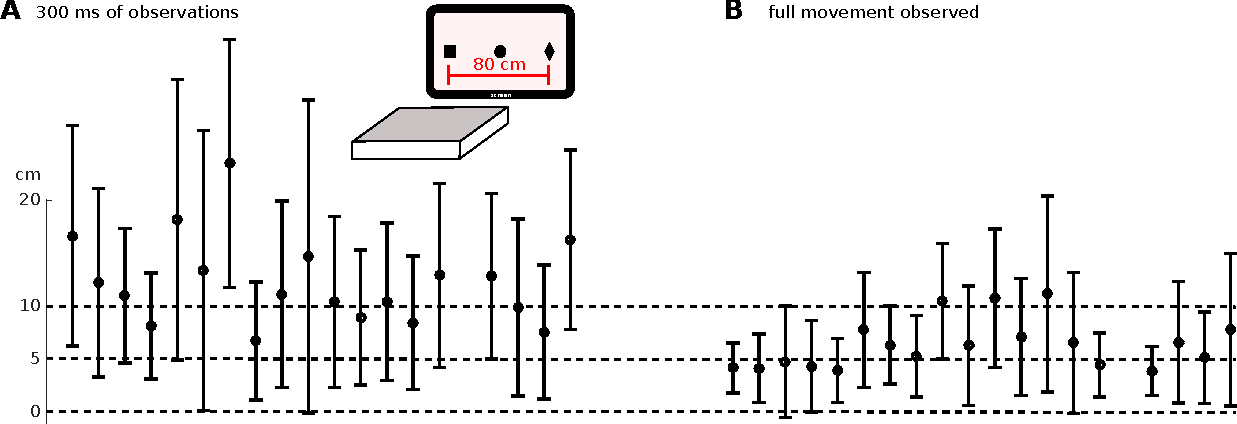
\includegraphics[width=\textwidth]{Elmar/picsClean/SubFigPredError9DoF}
% %\label{fig:subfig2}
%  \caption{\textbf{Supplementary figure, Target prediction error:} 
%  The left panel shows the averaged prediction error for $19$ subjects when observing $300$ ms of the left wrist marker trajectories in perturbed trials. 
%  The right panel shows the prediction error when observing the whole left wrist motion. Illustrated are the mean and the 
%  standard deviation over $18$ test trials (six per target). One subject of $20$ was excluded as less than six trials per target were recorded. 
%  Note that the maximum error or the distance between the two outer targets in the screen is $80$ cm.
%  }
% \label{fig:subFigPerdErrorAllSubjects}
% \end{figure}

\begin{figure}
\centering
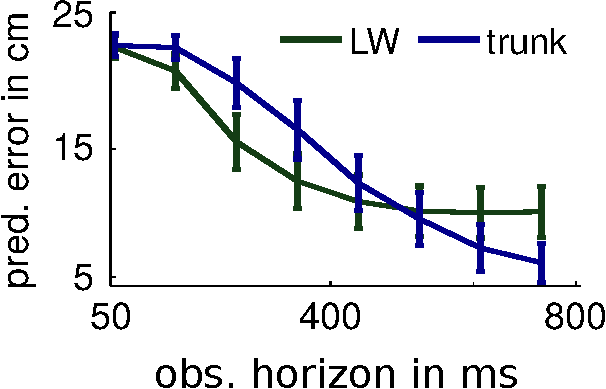
\includegraphics[width=.4\textwidth]{Elmar/picsSupp/SubFigPredErrorTrunkvsLW}
%\label{fig:subfig2}
 \caption{\textbf{Supplementary figure, Trunk vs. Left Wrist prediction error:} 
 Average prediction error in cm over all subjects given the left wrist (LW) or the trunk motion as observation. 
 }
\label{fig:SubFigPredErrorTrunkvsLW}
\end{figure}



\begin{figure}
\centering
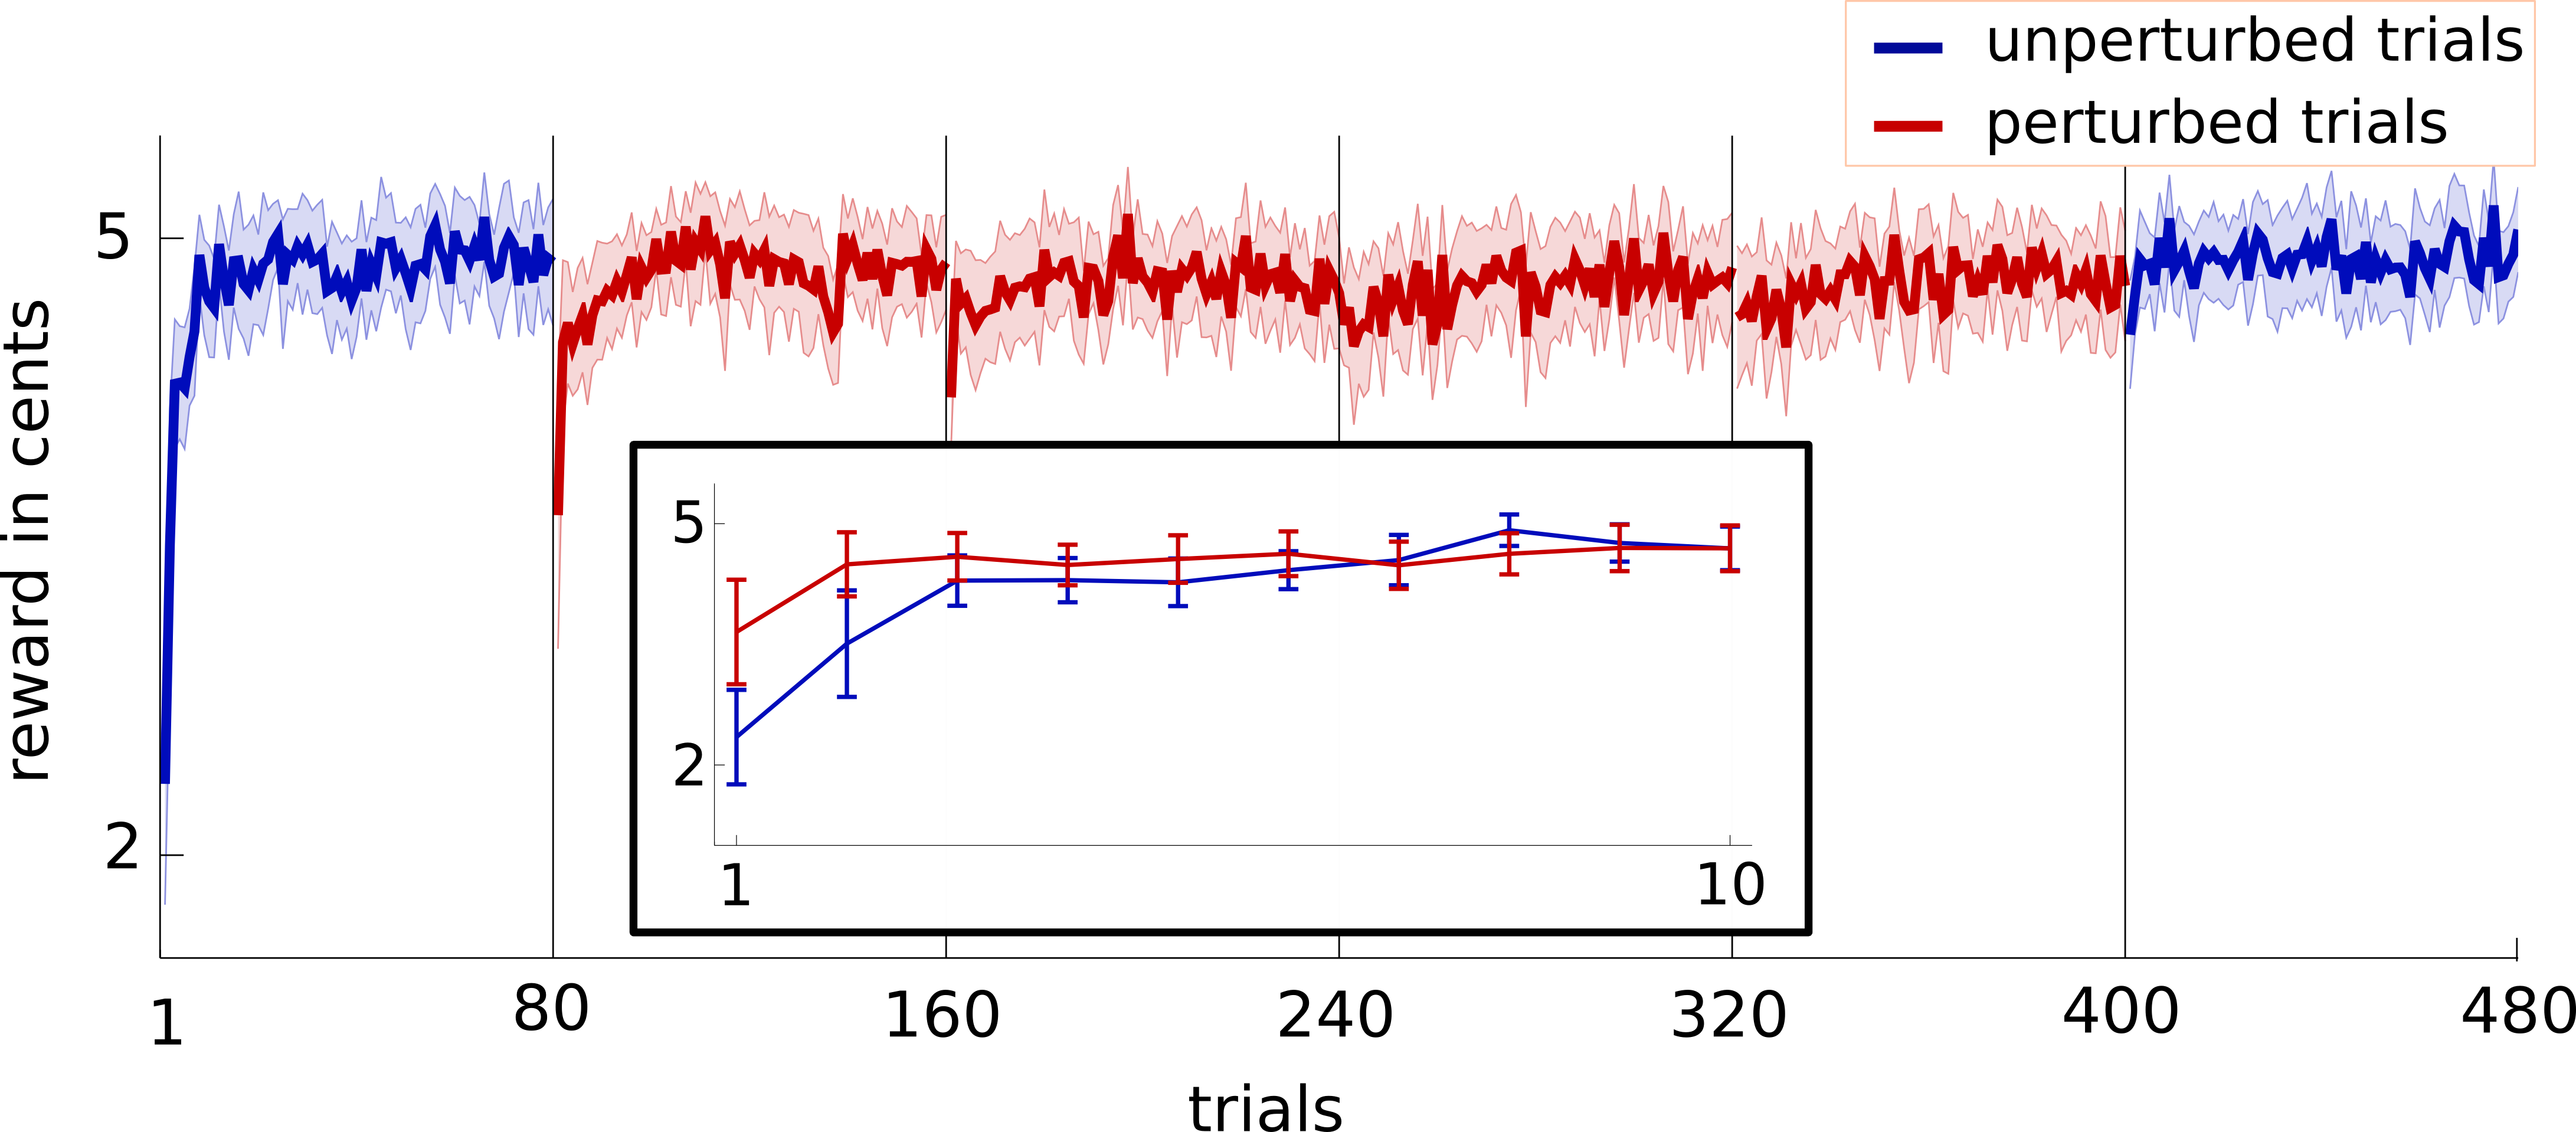
\includegraphics[width=\textwidth]{Elmar/picsSupp/FigRewards}
%\label{fig:subfig2}
 \caption{\textbf{Supplementary figure, Monetary rewards received: } 
 Illustration of the received rewards averaged over all $20$ subjects. The shaded region denotes the confidence bound. 
 }
\label{fig:SubFigRewards}
\end{figure}


\chapter{Use of rigid contacts during continuous perturbations}\label{sec:Jernej}
\renewcommand{\thesection}{\arabic{section}}  
\renewcommand{\thetable}{\arabic{table}}  
\renewcommand{\thefigure}{\arabic{figure}} 
\renewcommand{\theequation}{\arabic{equation}} 


Standing balance in human everyday environment is often exposed to
unpredictable and continuous external perturbations.  Moreover, when postural
control is impaired or challenged, handrails, canes, and handles are often
used to assist maintaining balance and the effects of these firm supportive
contacts in such conditions should be considered.  Therefore, we examined
changes in postural control in response to continuous, unpredictable
perturbations and explored the effect of using a handle as a supportive
contact.  Postural control of standing subjects was assessed with measurements
of centre of pressure (COP), which we also compared with perturbation waveform
and forces exerted on the handle, to check for correlations.  Kinematic data
were used to determine changes in posture and electromyographic data to define
the magnitude of muscle activity.  The use of handle affected the control of
posture by reducing the excursions of COP.  The reduction was found to be more
reflective in the posterior direction of COP excursions and was also in line
with higher forces exerted on the handle in the same direction.  The change of
posture was immediate when the contact to the handle was omitted and
significantly different between the two conditions.  Muscle activation levels
of the trunk flexor were significantly higher in the hand supported trial.  In
summary, we found that subjects clearly relied on using the handle for
support, even though the perturbations did not pose a significant balance
threat.  Results of direction specific control of posture with hand support
can be considered in rehabilitation and fall prevention programmes.


\section{Introduction}
Postural control is one of the vastly investigated area of human motor control in the last few decades. Most of the research on postural control focused on the role of sensory input in maintaining postural control during quiet standing, and in response to external balance perturbations. However, in our daily lives handrails, canes and handles are often used to assist maintaining balance, since they provide additional supportive contacts with the environment.
With respect to the use of hand contacts for postural control, one of the most investigated phenomena is "light touch" \cite{Jeka1997,Krishnamoorthy2002}. These light, fingertip contacts with stationary objects provide an additional sensory input, which helps individuals to better position them in space \cite{Jeka1997}. Furthermore, a more accurate sensory information improves postural control by reducing the amplitude of the centre of pressure (COP) movement \cite{Jeka1997,johannsen2007effects,Kouzaki2008,Wing2011a}.
However, hand contacts can serve as more than just sensory input. In situations where balance is exposed to larger perturbations, such as experienced on a moving bus or train, a firm hand contact (i.e. holding) is needed, as it provides a much better stabilising potential than a light touch \cite{Maki1997}. Holding to a handle, besides increasing the base of support of a standing individual, also enables generation of forces at the hand to counteract such perturbations \cite{Sarraf2014,Babic2014b}. For this, the location of the handle with respect to the subject’s position is important. Babič et al. \cite{Babic2014b} recently found that handle position relative to the subject, along with support surface perturbation direction and intensity, has a significant effect on the maximal forces exerted at the handle during support surface perturbations in quiet standing. More specifically, lower forces exerted at handles located at shoulder and eye level were needed to maintain a comparable peak displacement of the COP. This indicates that handles were used for postural control irrespective of their position, but certain handle positions could be exploited more efficiently.
Previously mentioned studies all based on discrete perturbations of balance. Such perturbations evoke reactive postural responses and conclusions were made on the basis of these responses. However, a major component of such responses is comprised of motor actions that are related to various sensorimotor reflexes and in less extent to the voluntary component of the postural control [13].
In contrast to discrete perturbations, continuous perturbations involve both reactive and proactive components of motor actions and in this sense offer a complementary insight into the postural control. Therefore, in this research we focused on changes in postural control during continuous perturbations of subject's balance. We aimed to record the mechanical function of the arm in a function of whole body balance stabilization to measure the effect of a firm hand contact on postural control.


\section{Methods}
We measured thirteen healthy right-handed young adults (average age = 22.2 years, SD = 2.2 years, average height 179 cm, SD = 6.2 cm and average weight = 76.7 kg, SD = 8.4 kg). The study was previously approved by the National medical ethics committee (No. 112/06/13) and all subjects participated after giving their written consent. Data of three subjects were  excluded from the analyses due to some technical issues.

\subsection{Experimental protocol}
Subjects were standing on a force plate while their standing balance was being perturbed for 5 minutes by a motorized waist-pull system \cite{Peternel2013} (\FigureAbbr \ref{fig:methods}). They were required to keep upright with their feet placed at hip width, look straight ahead, and maintain balance without making any unnecessary corrective steps. The experiment consisted of two conditions: balancing with ("with handle"; WH) and without ("no handle"; NH) holding onto a handle. In the WH condition subject held onto a stationary handle (diameter $=$ 3.2 cm, length $=$ 12 cm) positioned at shoulder height \cite{Babic2014b} with their right hand. In the NH condition subjects were standing freely with their arms folded across their chest. 
Balance was perturbed using a random white noise signal constructed to emulate mild, daily life perturbations (e.g., public transport) bus and avoid large, abrupt, and startling balance perturbations. This perturbation signal was based on pilot experiments, had a frequency range between 0.25 and 1.00 Hz and the maximum perturbation force of 11\% of the subject's body weight. 
Kinetic data were collected using a force plate (9281CA, Kistler Instrumente AG, Winterthur, Switzerland) under the subjects’ feet and a 3-axis force sensor (45E15A, JR3, Woodland, USA) on the base of the handle, both at 1000 samples/s. Unilateral  (right hand side) kinematic data were collected at a sampling rate of 100 samples/s using a contactless motion capture system (3D Investigator, Northern Digital Inc., Waterloo, Ont., Canada) consisting of a 3$\times$3 camera array. Seven active markers were attached on the subject's right 5th metatarsal-phalangeal, ankle, knee, hip, shoulder, elbow and wrist joint. Electromyographical (EMG) activity of the right leg (Tibialis Anterior; TA, Gastrocnemius lateralis: GA) and of the trunk (Multifidus; MF, Obliques Externus; OE) was measured using Biometrics DataLOG MW8X at a sampling rate of 1000 samples/s. 
Before the start of the experiment, subjects performed three maximal voluntary contractions (MVC) of each of the measured muscles and were exposed to 14 trials of 5 minutes of the WH condition. The aim of these preparatory WH trials was to familiarize the subjects with the experimental set-up and avoid any learning effects observed in previous balance experiments.

\begin{figure}[htb!]
	\centering
	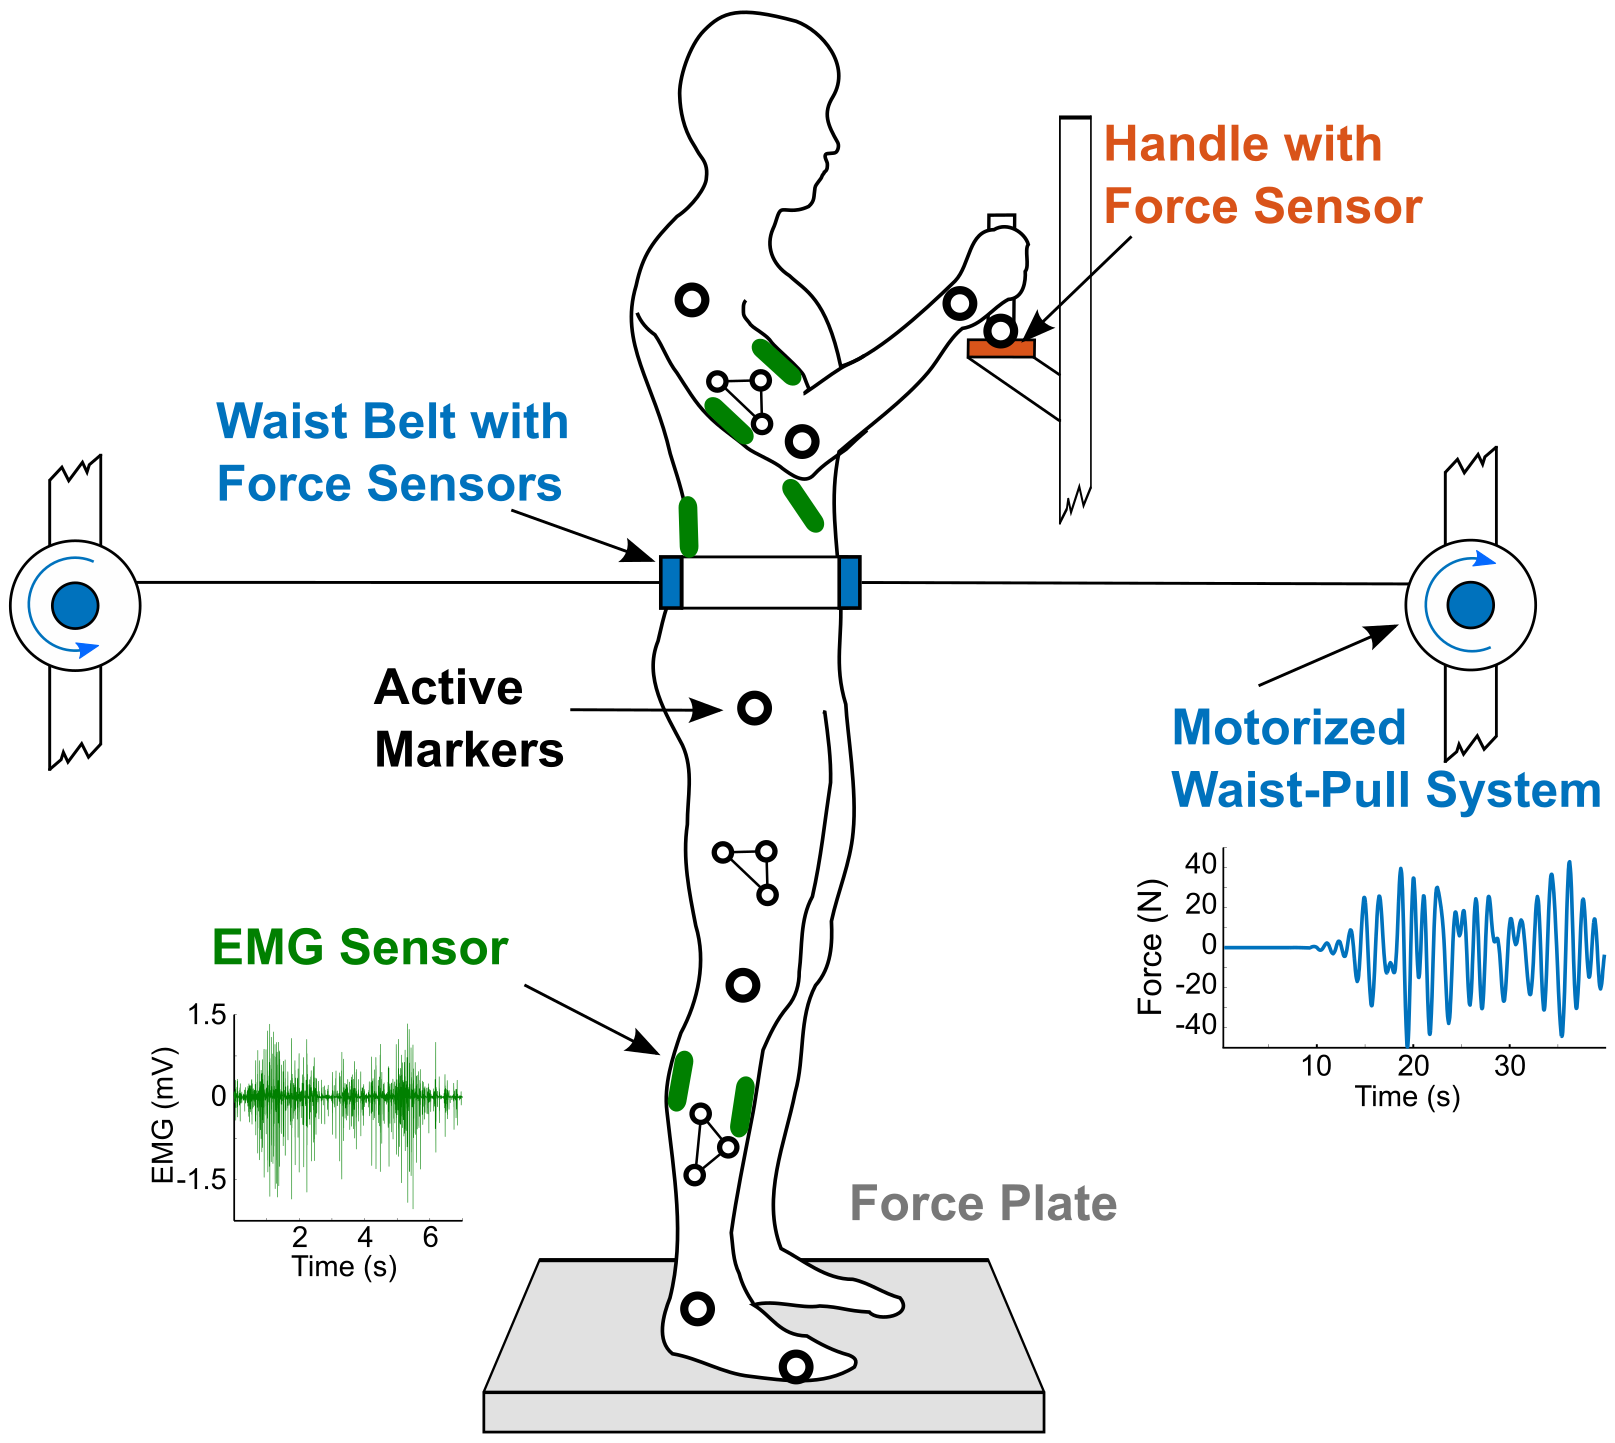
\includegraphics[width=0.85\textwidth]{Jernej/figures/expSetup}
	\caption{\textbf{Experimental setup. }The subject is standing on a force plate, wearing a waist belt connected to the motorized waist-pull system which generated translational force perturbations in the anterior-posterior direction using a random white noise signal constructed to emulate mild, daily life perturbations. The actual perturbation waveform is shown on the plot below the motorized waist-pull system.
			}
	\label{fig:methods}
\end{figure}

\subsection{Data analysis}  
Anteroposterior  displacement of the subject’s centre of pressure (COP) was calculated from the data provided by the force plate on which the subjects were standing. 
Kinematic data were low pass filtered (zero lag, 2nd order Butterworth algorithm, cut-off frequency 20 Hz) \cite{Bartlett1997} and ankle, knee, and hip joint angles were calculated from the joint markers coordinates. 
Mean values of joint angles over time were fitted using an exponential model $y = A^{e-t/\tau} + C$, where $A$ is the gain of the exponential process, $\tau$ is the time constant, $C$ is the offset, and $t$ refers to the trial number) to describe evaluation  of motor adaptation over time \cite{Franklin2003}. The onset of reaching a plateau (adaptation stabilized) was defined by calculating point in time at the three time constants (3$\tau$) of the fitted exponential curve. This is the point when the function reaches a value of less than 5\% of its starting value and was considered as the adaptation stabilized. 
EMG was band-pass filtered (zero lag, 2nd order Butterworth algorithm, with cut-off frequencies of 20 and 450 Hz), full-wave rectified and normalized by division with the MVCs.  By applying a low pass filter (zero lag, 2nd order Butterworth algorithm, 10 Hz cut-off frequency), we created envelopes of EMG signals and then integrated them over time, to observe the accumulated EMG activity.
\subsection{Statistical analysis}
To compare the NH and WH conditions we calculated the average COP displacement, hip, knee, and ankle angles and contact forces exerted on the handle over the 5 minutes for each subject. These individual average values were used for statistical analysis. 
We used paired samples t-test analysis to investigate the differences between the WH and NH conditions and linear correlation to investigate the relationship between the COP displacement and the magnitude of the perturbation (separately for anterior and posterior directions) and between COP and the exerted handle contact force. All statistical analyses were performed using SPSS 21 Inc., Chicago, USA and statistical significance was set at $\alpha =$ 0.05. The effect size (\textit{d}) was calculated by using standard Cohen’s equation ($\hat{d}=\dfrac{\bar{X}_{1} - \bar{X}_{2}}{s}$) \cite{Cohen1988}. 

After comparing the two trials we checked for direction specific differences of COP displacement within each trial. For this, we used a paired samples t-test on averaged measures of anteroposterior COP displacement. The relationship between the perturbation and the COP displacement was investigated in more detail by correlating the perturbation force and COP displacement and by correlating perturbation force and forces on the handle.

\section{Results}
Average anteroposterior displacements of the COP during the NH and WH conditions are shown in \FigureAbbr \ref{fig:cop}. In both conditions COP displacement was larger in the anterior direction (mean $\pm$ SE: NH 38.45 $\pm$ 1.6 mm,  WH 18.15 $\pm$ 1.2 mm) compared to posterior (mean $\pm$ SE: NH $-$34.88 $\pm$ 2 mm, WH $-$11.02 $\pm$ 1.5 mm), but this difference was significant only for the WH condition (\textit{t}(9) $=$ 2.81, \textit{p} $=$ .02, \textit{d} $=$ 1.52). Hence, the remainder of our COP analyses were conducted for the anterior and posterior directions separately. 

Overall, COP displacements were significantly larger in the NH condition compared to WH condition, both in the anterior (difference of 20.3 mm, \textit{t}(9) = 7.78, \textit{p} = .001, \textit{d} = $-$4.15) and posterior direction (difference of 23.9 mm, \textit{t}(9) = $-$11.09, \textit{p} = .001, \textit{d} = $-$3.8). 

\clearpage
As can be seen from \FigureAbbr \ref{fig:corr}A, the correlation between the COP displacement and perturbation force was \textit{r}$_{p} =$ .77 (\textit{p} $<$ .001) and \textit{r}$_{a} =$ .82 (\textit{p} $<$ .001) in the NH condition for the posterior and anterior direction, respectively. For the WH condition (\FigureAbbr \ref{fig:corr}B) the correlations were \textit{r}$_{p} =$ .67 (\textit{p} $<$ .001) and \textit{r}$_{a} =$ .89 (\textit{p} $<$ .001) for the posterior and anterior direction, respectively.

\begin{figure}[!htb]
	\centering
	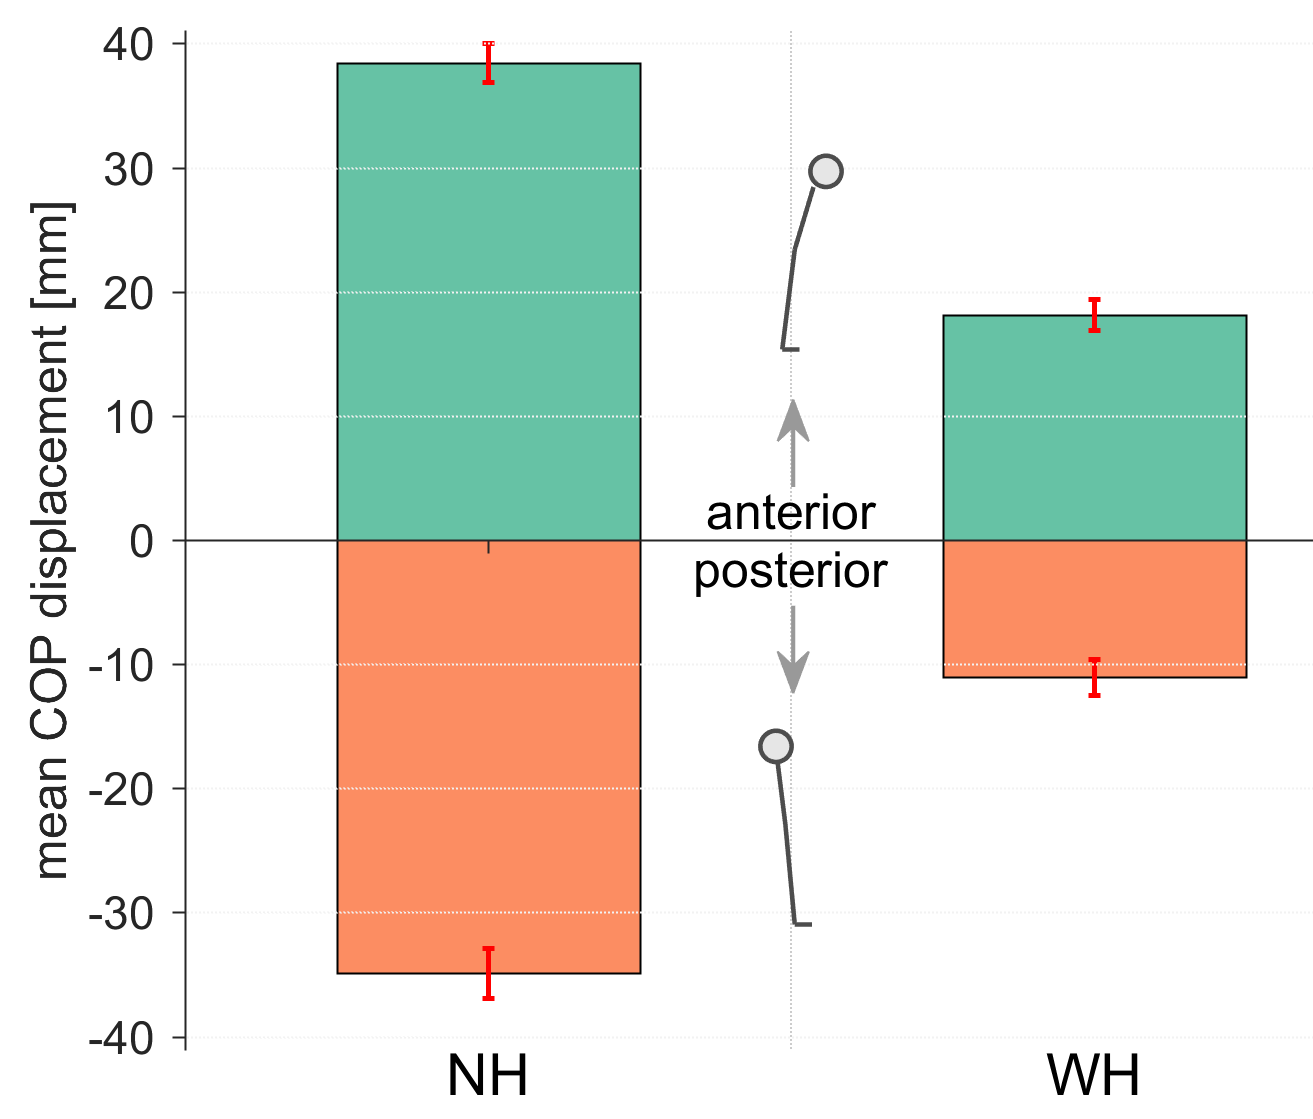
\includegraphics[width=0.7\textwidth]{Jernej/figures/cop}
	\caption{\textbf{Anteroposterior displacement of COP. }Mean COP displacement in NH and WH trials, for the anterior (positive) and posterior (negative) directions. Error bars indicate $\pm$ 1 standard error of the mean.
	}
	\label{fig:cop}
\end{figure}

Correlations between the forces exerted on the handle and the perturbation force (\FigureAbbr \ref{fig:corr}C) were large in both anterior (\textit{r}$_{p}$ $=$ .85, \textit{p} $<$ .001) and posterior direction (\textit{r}$_{a}$ $=$ .81, \textit{p} $<$ .001). However, the slope of a least-squares linear fit to the data indicates, that subjects utilized the handle considerably more for perturbations in the posterior direction (k$_{p}$ = 1.3) than for perturbations in the anterior direction (k$_{a}$ = .86).

\clearpage
\begin{figure}[!htb]
	\centering
	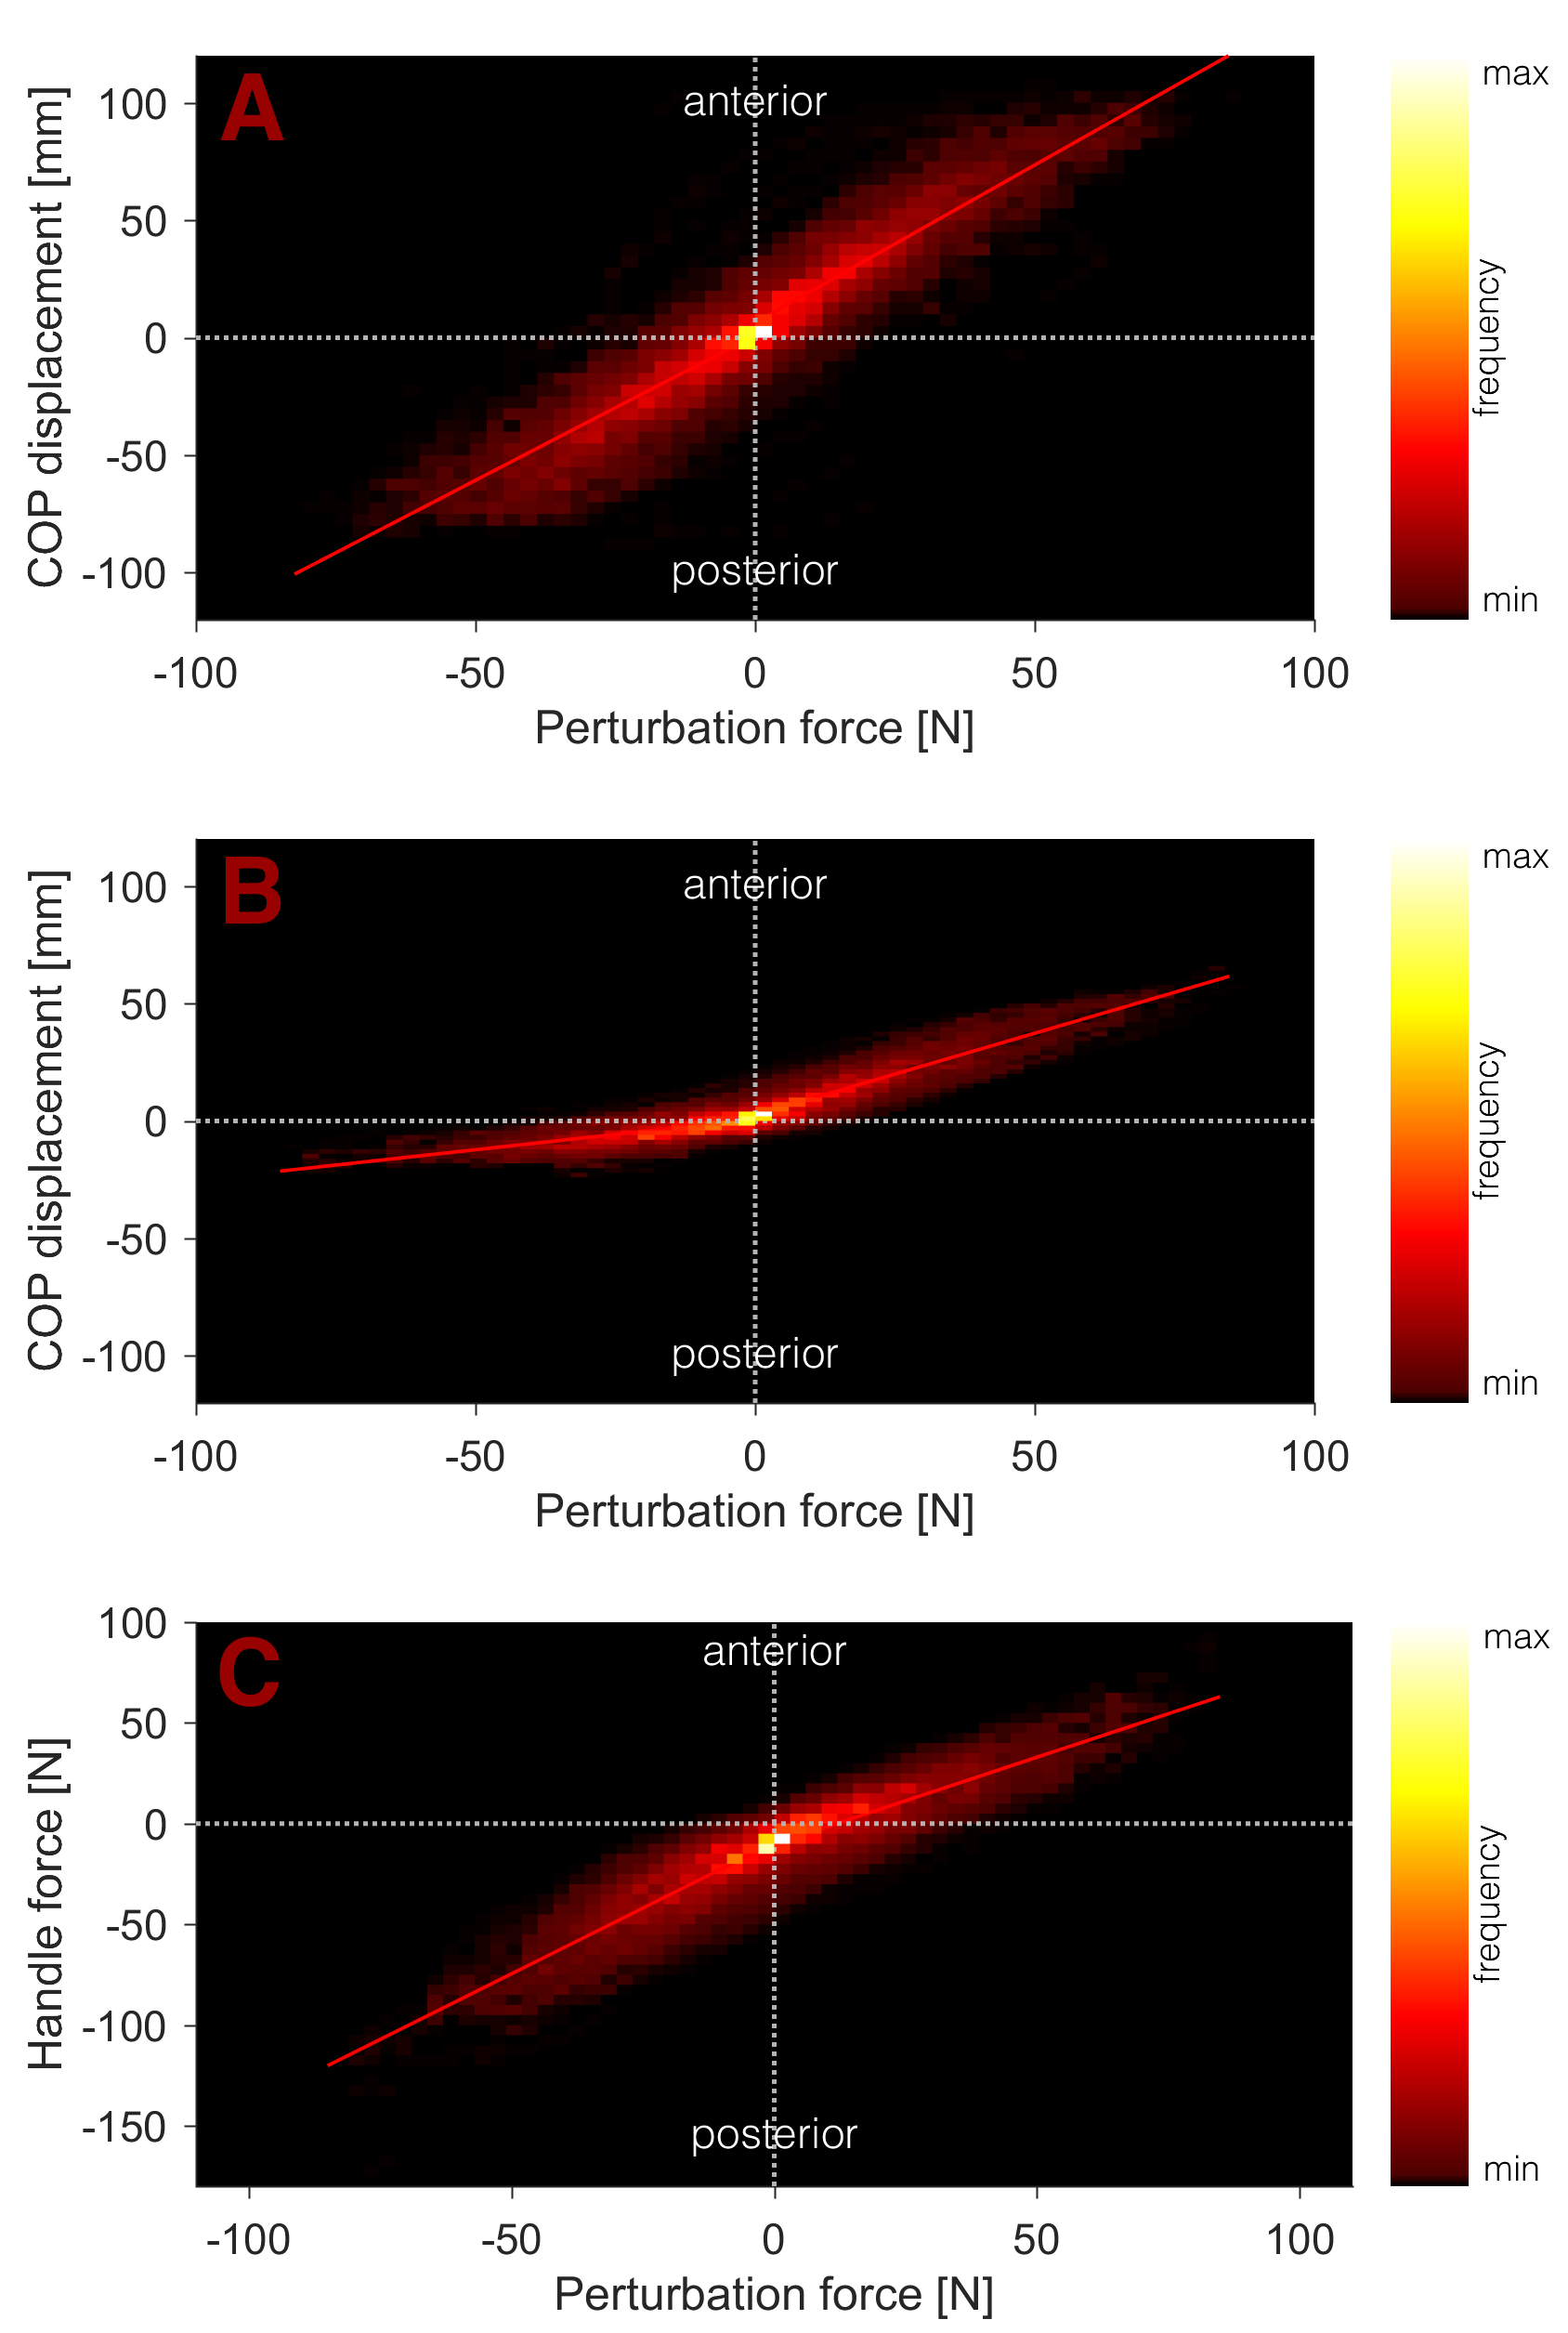
\includegraphics[width=0.7\textwidth]{Jernej/figures/corr}
	\caption{\textbf{Correlation. }\textbf{(A)} Correlation between the perturbation force and COP displacement in the NH condition, \textbf{(B)} correlation between COP displacement and perturbation force in the WH condition, and \textbf{(C)} correlation between handle force and perturbation force in the WH condition.  All correlations were calculated separately for the anterior (positive) and posterior (negative) direction.
	}
	\label{fig:corr}
\end{figure}

Joint angles prior to the start of perturbation were significantly smaller in the NH condition compared to WH condition (\FigureAbbr \ref{fig:jAnglesBars}). Differences were the largest in the knee (mean $\pm$ SE: 169.4 $\pm$ 1.4$^{\circ}$ for NH, 172.9 $\pm$ 1.4$^{\circ}$ for WH, \textit{t}(9) $= -$4.05, \textit{p} $=$ .01, \textit{d} $=$ 1.36 ), followed by the hip (mean $\pm$ SE: 179 $\pm$ 1.8$^{\circ}$ for NH, 181.6 $\pm$ 1.5$^{\circ}$ WH, \textit{t}(9) $= -$2.95, \textit{p} $=$ .024, \textit{d} $=$ 1.13), and ankle (mean $\pm$ SE: 110.4 $\pm$ 1.1$^{\circ}$ for NH, 112.1 $\pm$ 1.2$^{\circ}$ WH, \textit{t}(9) $= -$2.71, \textit{p} $=$ .038, \textit{d} $=$ 1.08).


\begin{figure}[!htb]
	\centering
	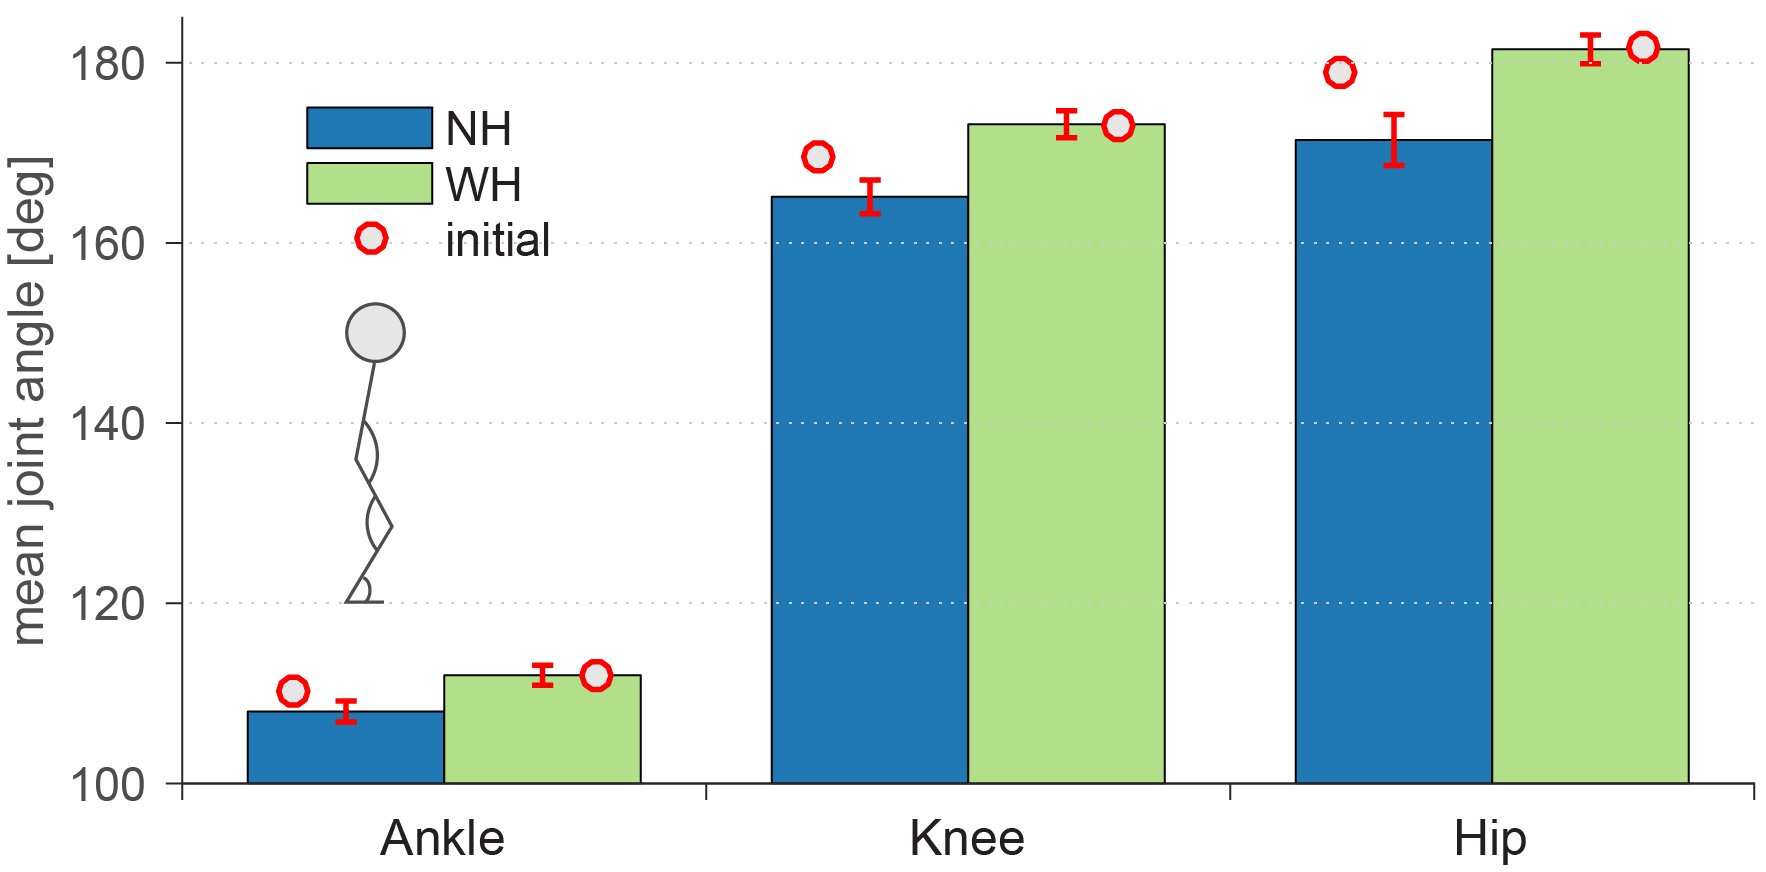
\includegraphics[width=0.7\textwidth]{Jernej/figures/jAnglesBars}
	\caption{\textbf{Ankle, knee and hip joint angles. }Mean value of joint angles during the perturbation is given for NH (blue bars) and WH condition (green bars) and mean joint angles prior to the start of perturbation are shown as red circles above bars. Error bars indicate $\pm$ 1 standard error of the mean.
	}
	\label{fig:jAnglesBars}
\end{figure}

Ankle (A), knee (B), and hip (C) angles over the time course of the perturbation are shown in \FigureAbbr \ref{fig:expFit}. Exponential curves fitted to the data show that mean joint angles in the NH condition changed after the perturbation onset before reaching a steady state. The steady state was reached first by the ankle angle (86 s after perturbation onset), followed by the knee angle (112 s after the perturbation onset) and finally hip angle (195 s after the perturbation onset), resulting in more ankle, knee and hip flexion.

\begin{figure}[!htb]
	\centering
	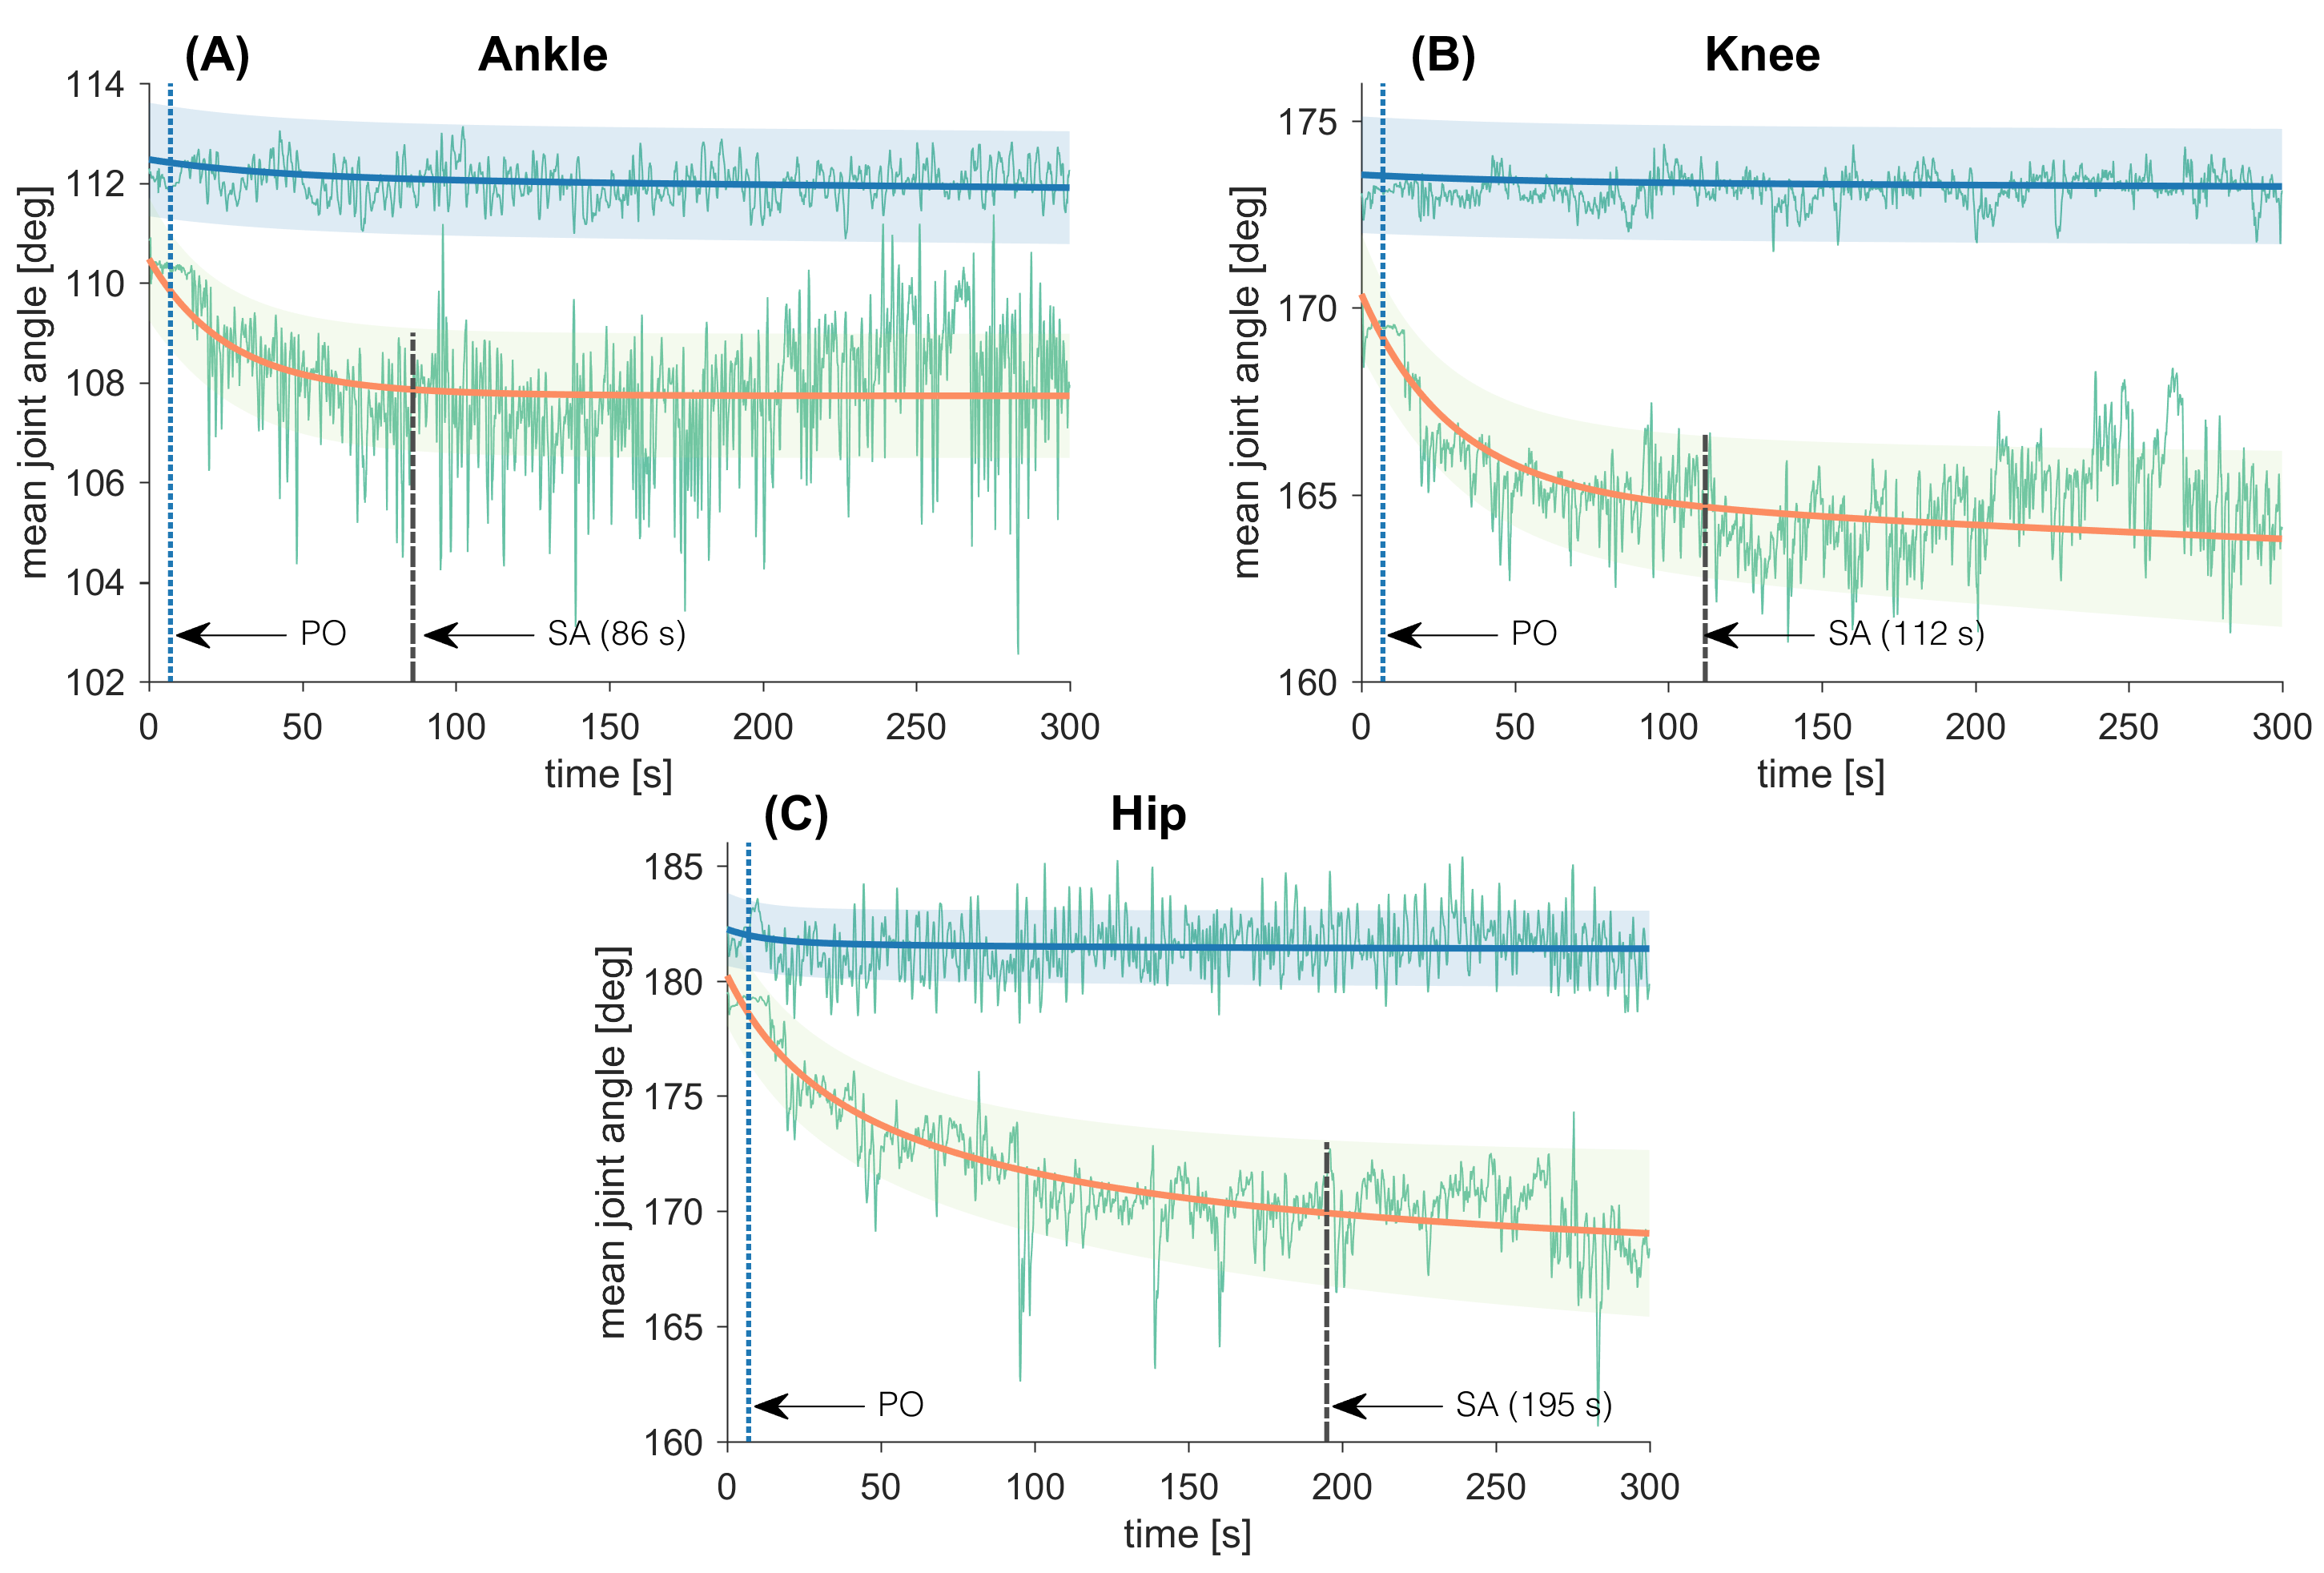
\includegraphics[width=0.92\textwidth]{Jernej/figures/expFit}
	\caption{\textbf{Ankle, knee and hip joint angles. }Figures represent mean ankle \textbf{(A)}, knee \textbf{(B)}, and hip \textbf{(C)} angles over the time course of the perturbation. Thin solid curves represent mean joint angles during NH and WH conditions. Thick solid lines represent exponential curve fit, denoting adaptation of joint angles in the NH (orange) and WH (blue) conditions, while shaded areas represent standard error of the mean. The dotted vertical lines represent perturbation onset (PO) while the dashed vertical lines indicate stabilized changes (adaptation) in the joint angles (SA).
	}
	\label{fig:expFit}
\end{figure}

\clearpage
Finally, muscle activity is significantly lower during the WH condition than during the NH condition both for the leg muscles (GA \textit{t}(9) $=$ 3.57, \textit{p} $=$ .04, \textit{d} $= -$0.89; TA \textit{t}(9) $=$ 6.41, \textit{p} $=$ .002, \textit{d} $= -$1.85) and trunk muscle (MF \textit{t}(9) $=$ 6.5, \textit{p} $=$ .001, \textit{d} $= -$1.01), as can be seen in \FigureAbbr \ref{fig:iemg}. 
Leg muscle activity is lower for 18.4 $\pm$ 4.9\% in the GA (mean $\pm$ SE: NH: 28.97 $\pm$ 6.5\% MVC, WH: 10.6 $\pm$ 2.3\% MVC) and for 23.7 $\pm$ 3.5\% in the TA (mean $\pm$ SE: NH: 27.21 $\pm$ 4\% MVC, WH: 3.47 $\pm$ 1.9\%), while trunk muscle activity is lower for 14.3 $\pm$ 2.1\% in the MF (mean $\pm$ SE: NH: 36.17 $\pm$ 4.5\% MVC, WH: 21.83 $\pm$ 3.7\%).

\begin{figure}[!htb]
	\centering
	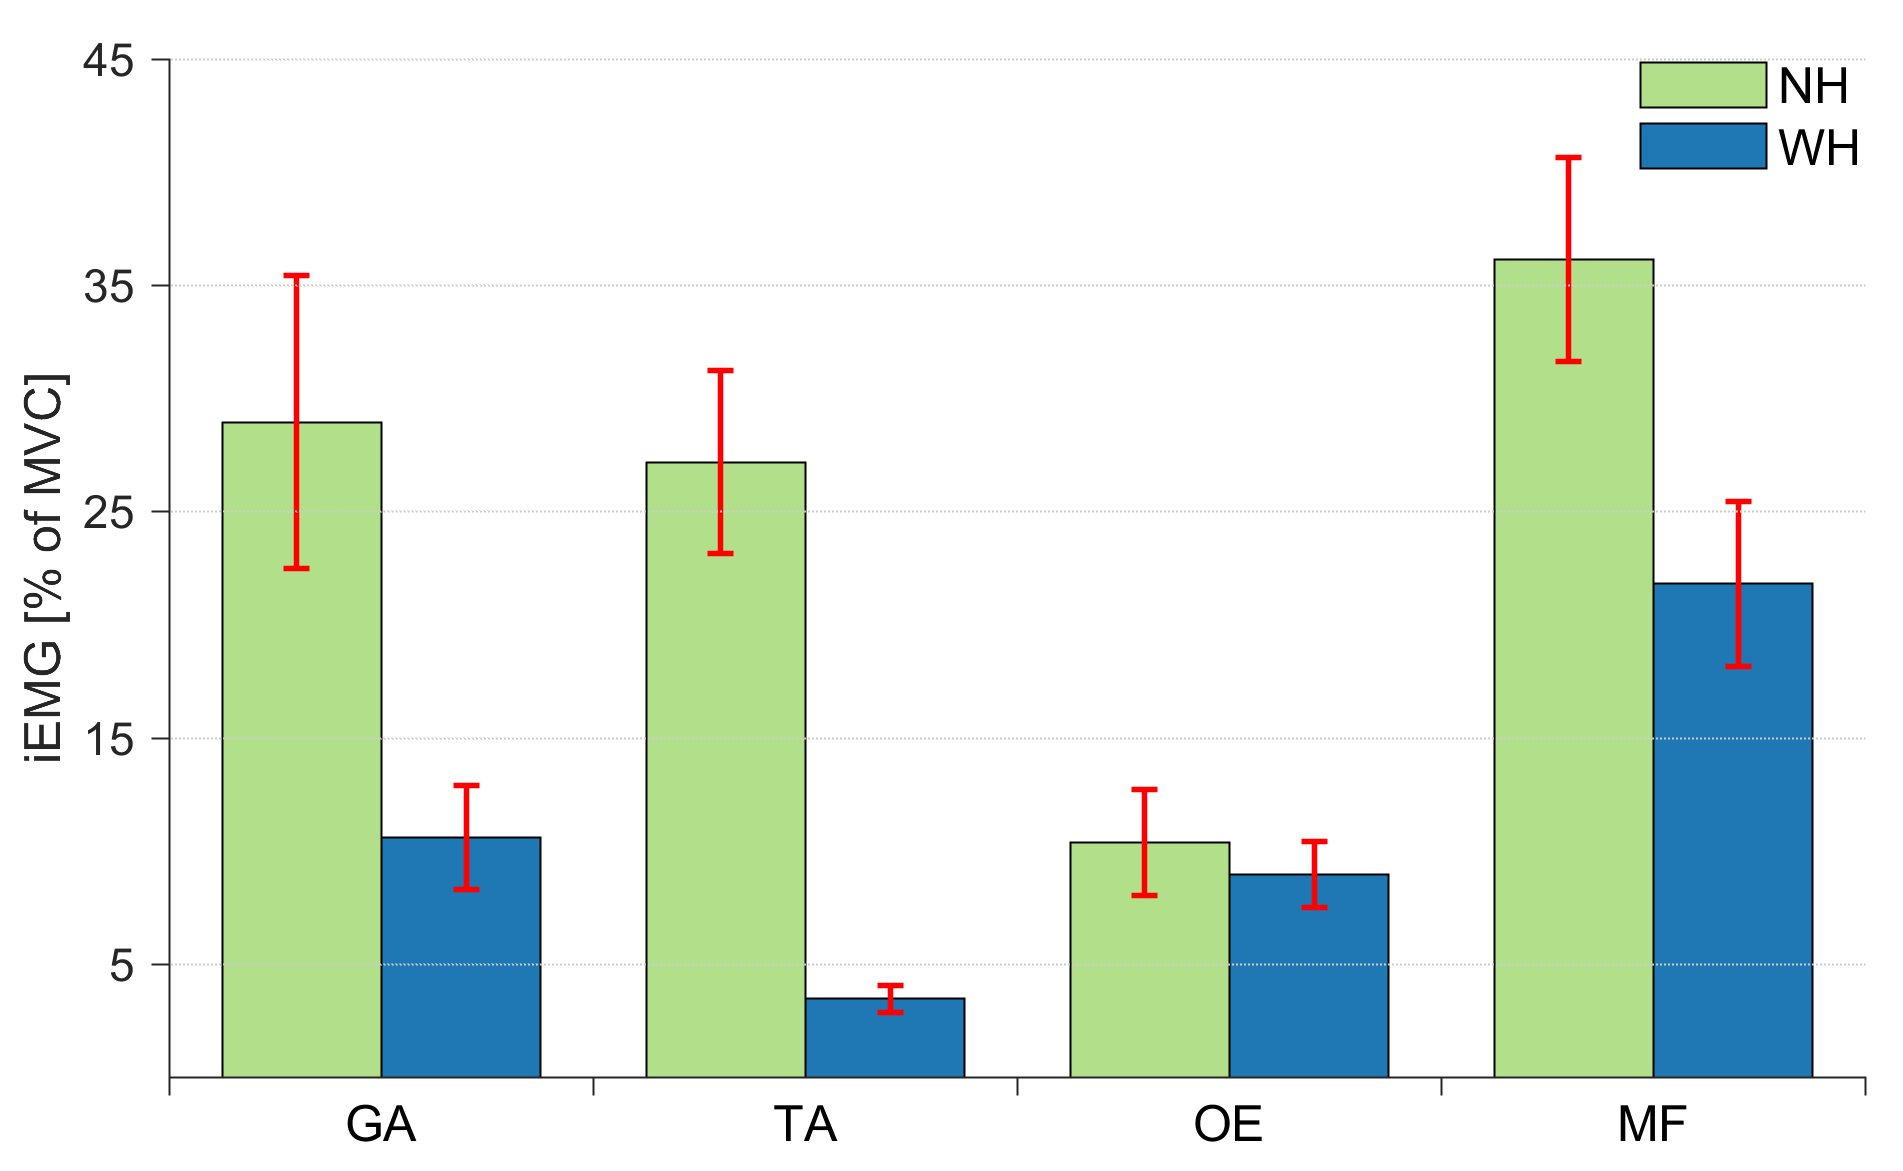
\includegraphics[width=0.7\textwidth]{Jernej/figures/iemg}
	\caption{\textbf{Muscle activity. }Mean integrated EMG activity of leg (GA and TA) and trunk (OE and MF) muscles during the NH (green bars) and WH condition (blue bars). Error bars indicate $\pm$ 1 standard error of the mean.
	}
	\label{fig:iemg}
\end{figure}


\section{Conclusions}
Standing balance in human everyday environment is often exposed to unpredictable and continuous external perturbations. Moreover, when postural control is impaired or challenged, handrails, canes, and handles are often used to assist maintaining balance and the effects of these firm supportive contacts in such conditions should be considered.
Therefore, we examined changes in postural control in response to continuous, unpredictable perturbations and explored the effect of using a handle as a supportive contact. Postural control of standing subjects was assessed with measurements of centre of pressure, which we also compared with perturbation waveform and forces exerted on the handle, to check for correlations. Kinematic data were used to determine changes in posture and electromyographic data to define the magnitude of muscle activity.
COP displacement, hip, knee, and ankle angles, leg and trunk muscle activity and handle contact forces were analysed for the anterior and posterior directions separately, as COP displacement was significantly larger in the anterior direction (WH, 7 mm, \textit{p} $=$ .02). Perturbation force was strongly correlated to COP displacement (all r $>$ .65) and handle forces (r $>$ .8) in both directions. COP displacement was significantly larger in the NH condition compared to WH condition (anterior: 20 mm, posterior: 24 mm, both \textit{p} $=$ .001) and regression indicated that subjects utilized the handle slightly more for posterior perturbations. In the NH condition, all joint angles decreased in anticipation of the perturbation (2-4$^{\circ}$, all \textit{p} $<$ .04) and until 86-195 s following perturbation onset. Finally, leg (18-24\%) and one of the trunk (14\%) muscles increased their activity in the NH condition (all \textit{p} $\leqslant$ .04). 
In summary, we found that subjects clearly relied on using the handle for support, even though the perturbations did not pose a significant balance threat. Results of direction specific control of posture with hand support can be considered in rehabilitation and fall prevention programs.


\chapter{Learning compliant contacts}\label{sec:Chie}

\section*{Abstract}

Abstract goes here


\section{INTRODUCTION}

Write a short introduction


\section{name the section}

\subsection{if you need any subsection}


\section{Results or Discussions}

This is how you put a pictue:
\begin{figure}
  \centering
  \caption{explanation}
  \includegraphics[width=0.95\linewidth]{Chie/figs/stance.png}
  \label{label for referencing}
\end{figure}




\bibliographystyle{plain}
\bibliography{manuscriptAll,rigidContacts}




\end{document}

%%% Local Variables:
%%% mode: latex
%%% TeX-master: t
%%% save-place: t
%%% End:
